% ============================================================
% Paper 30 v3 -- reading draft (2026-11-06; revised 2026-11-06 after internal review: H1 reframed, new arXiv paper)
% Template: PRIMEarxiv (copied from paper 33, /data/heretic_2/33_2611_does_refusal_removal_get_harder/paper/main.tex)
% Build: pdflatex main.tex && bibtex main && pdflatex main.tex && pdflatex main.tex
% Numbers: every number comes from ../analysis/*.csv (assemble_p30.py); tables are generated by
%   ../scripts/make_tables.py, figures by ../scripts/make_figures.py; supplementary statistics by
%   ../scripts/supp_stats.py (-> ../analysis/supp_stats.csv).
% ============================================================
\documentclass{article}

\usepackage{PRIMEarxiv}
\usepackage[utf8]{inputenc}
\usepackage[T1]{fontenc}
\usepackage{url}
\usepackage{booktabs}
\usepackage{array}
\usepackage{multirow}
\usepackage{graphicx}
\usepackage{float}
\graphicspath{{figures/}}
\usepackage{amsfonts}
\usepackage{amsmath}
\usepackage{amssymb}
\usepackage{nicefrac}
\usepackage{microtype}
\usepackage{xcolor}
\usepackage{colortbl}
\usepackage{fancyhdr}
\usepackage{hyperref}
\hypersetup{colorlinks=true, linkcolor=blue, citecolor=blue, urlcolor=blue,
  pdftitle={Comparing Abliteration Tools Under Held-Out, Judge-Based Evaluation}, pdfauthor={Richard J. Young}}

\raggedbottom

% --- Draft markers (remove before submission: grep -n todo sections/*.tex) ---
\newcommand{\todo}[1]{\textcolor{red}{[TODO: #1]}}

\pagestyle{fancy}
\thispagestyle{empty}
\rhead{\textit{ }}
\fancyhead[LO]{Comparing Abliteration Tools Under Held-Out, Judge-Based Evaluation}

\title{Comparing Abliteration Tools Under Held-Out, Judge-Based Evaluation:\\ Heretic 1.x, Heretic 2.0 and Community Releases\\ on Qwen2.5}

\author{
  Richard J. Young \\
  University of Nevada Las Vegas \\
  Department of Information Systems \\
  Las Vegas, NV, USA \\
  \texttt{ryoung@unlv.edu} \\
}

\begin{document}
\maketitle

\begin{abstract}
% ABSTRACT (150--250 words, excluding the red draft line). Rewritten 2026-11-06 (reading draft v3) after the 7B 1.x
% cells, the KL<=0.1 re-export of the 1.x general study on Qwen2.5-32B and the external-tool cells were judged.
% Numbers (all from analysis/, assemble_p30.py run 2026-11-06T22:47Z):
%   up to 73.1 pp: RESULTS.md "Modified vs original" (12 1.x cells; max 73.1 = qwen2.5-coder-14b 1.x general; the
%     minimum, qwen2.5-7b 1.x code -0.9 [-2.3,+0.4], p_Holm 0.222, is not significant, hence "up to", not "0.9--").
%   H1: RESULTS.md "H1" / tests_refusal.csv family h1_1x_vs_2.0, wg harmful_all: 32B 73.4 vs 47.4, +25.9 [23.0, 28.7];
%     7B 39.6 vs 20.6, +19.0 [16.1, 21.9]; both p_Holm<0.001.
%   Ten-fold cap: 1.x rule KL<=0.01 vs 2.0 rule KL<=0.1 (04_methods tab:h1setup; dev_matched_kl.csv selection_cap).
%   KL-matched: RESULTS.md "1.x general re-exported at KL <= 0.1" / tests_refusal.csv family h1_kl_matched:
%     cells.csv qwen2.5-32b__heretic1x-general-kl0.1 wg 11.6 [9.8, 13.8]; vs DiM -35.8 [-38.9, -32.7];
%     vs MPOA +7.7, vs ARA +5.6 (MPOA 3.9%, ARA 6.1%); all p_Holm<0.001.
%   External: RESULTS.md "Added cells vs their original" + cells.csv: obliteratus-basic 72.9 vs base 72.1
%     (+0.8 [-0.6,+2.3], p_Holm 0.332); spectral_cascade 11.8, capability mean delta -5.18 [-6.90,-3.47]
%     (tests_capability.csv family added); jwest33 qwen3.5-4b as released 1.0 (primary), hybrid fix 35.8.
%   H2: tests_refusal.csv h2_general_vs_code (no crossover in 6 models; 32B code_weapon_excl_risk n.s.).
%   H3: tests_refusal.csv kw_vs_judge, kw_minus_wg, max +19.5 (qwen2.5-7b DiM), original-design cells.
% Word count 250 (numbers and intervals counted as one word each).
\noindent\textcolor{red}{\textbf{Reading draft v3, 6 November 2026.}}\par\medskip

\noindent Abliteration tools remove refusal from open-weight language models by editing weights, and
practitioners choose among tools, versions and settings mostly from keyword-matched refusal counts on tuning
prompts. This study rebuilt archived Heretic~1.x models with general- and code-derived refusal directions for six
Qwen2.5 models and evaluated them, alongside Heretic~2.0, two external tools at their documented settings and two
community releases, on 972 held-out harmful prompts, scored by a safety judge, and five capability benchmarks.
Twelve 1.x models removed up to 73.1 percentage points (pp) of refusal. With the same edit,
Heretic~2.0 left less residual refusal than 1.x on Qwen2.5-32B (47.4\% versus 73.4\%; 25.9~pp [23.0, 28.7]) and
Qwen2.5-7B (20.6\% versus 39.6\%; 19.0~pp [16.1, 21.9]), but the archived 1.x runs had selected their output under
a ten-fold tighter divergence cap. Re-exported from the same Qwen2.5-32B search at the 2.0 cap, 1.x left 11.6\%
[9.8, 13.8], 35.8~pp [32.7, 38.9] less than its 2.0 counterpart and more than 2.0 MPOA (3.9\%) and ARA (6.1\%).
OBLITERATUS's basic preset left refusal unchanged (72.9\% versus 72.1\%) and its spectral-cascade preset reached
11.8\% with a 5.2-pp capability loss; jwest33's abliterator left 1.0\% on Qwen3.5-4B as released and 35.8\% with
hybrid-architecture detection restored. A code-derived direction gave no consistent advantage on malicious-code
prompts, and keyword matching counted up to 19.5~pp more refusals than the judge. Tool comparisons should therefore
report the selection rule and the released model's divergence. On Qwen2.5-32B, the newer version's apparent
advantage reflected the selection cap rather than the version.

\end{abstract}

\keywords{Abliteration \and Refusal Removal \and Heretic \and Open-Weight LLMs \and LLM Safety Evaluation \and Benchmarking}

% =====================================================================
% 1 INTRODUCTION (house pattern: problem | known | gap | purpose + hypotheses)
% Revised 2026-11-06: H1 = like-for-like contrast (1.x general vs 2.0 DiM); SOM and J-space labelled as
% project-fork plug-ins; 2512.13655 presented as prior work (this is a new paper); positioning sentence added.
% Revised 2026-11-06 (draft v3): hypotheses unchanged. Added (i) the external tools to the design sentence,
% (ii) the KL<=0.1 re-export described as the check of the selection-cap explanation that the earlier draft had
% named as the decisive test (specified after the 32B H1 result, before the re-exported model was evaluated;
% not a new hypothesis), (iii) companion-cell count 13 -> 19 (13 Qwen2.5 cells + Qwen3.5-4B original and its five
% 2.0/fork cells; cells.csv provenance "paper 33" / ref_dir runs/mc-rtx-1), (iv) external tools descriptive only.
% =====================================================================
\section{Introduction}
\label{sec:intro}

Instruction-tuned language models with open weights are released with safety training that makes them refuse
harmful requests, and that refusal can be removed after release without further training. Abliteration edits the
weight matrices that write to the residual stream so that the model can no longer represent a refusal direction
\cite{arditi2024refusal,labonne2024abliteration}, and a growing set of open-source tools automates the edit
\cite{failspy_abliterator,erisforge,jimplus_llmabliteration,heretic2025,obliteratus2026,jwest33abliterator}.
Researchers who study refusal, red-teamers who need unfiltered baselines and auditors who estimate how easily a
release can be stripped of its safeguards must therefore choose a tool, a tool version, a method within the tool
and the rule that selects which edited model is released. The same choice made by a malicious actor determines how
much protection a release retains, so the relative effectiveness of these tools is a safety-relevant quantity
rather than a matter of convenience.

Refusal in many chat models is mediated largely by one direction in activation space \cite{arditi2024refusal}, and
successors of the original difference-in-means (DiM) edit project the direction away from the harmless mean
\cite{lai2024projected}, preserve weight-row magnitudes \cite{lai2025mpoa}, ablate several directions found by
self-organising maps \cite{piras2025som} or replace the direction with an optimised low-rank map
\cite{weidmann2026ara}. Heretic automates the choice of layers and strengths with a Bayesian search that trades
keyword-counted refusals against first-token Kullback--Leibler (KL) divergence \cite{heretic2025,akiba2019optuna}.
Its 2.0 release reorganised the tool around modifier and scorer plug-ins and added arbitrary-rank ablation (ARA)
as a built-in method; the direction-projection and row-normalisation options that define magnitude-preserving
orthogonal ablation (MPOA) were already available in 1.x builds. An earlier comparison \cite{young2025comparative} evaluated
four tools on sixteen 7--14B models and reported large differences in compatibility and in capability
preservation, for example a GSM8K loss of 18.8 percentage points (pp) for Heretic on Yi-1.5-9B against near-zero
losses for single-pass tools.

That comparison shared the measurement practice of the tools themselves. Refusal was counted with keyword markers on
100 prompts from the same AdvBench-derived dataset used to compute the refusal direction, each tool ran at its own
default settings, and distribution shift was summarised by the first-token KL divergence that the search itself
optimises. Keyword matching agrees poorly with human labels and with model-based judges
\cite{xie2025sorrybench,young2026measuring}, and after ablation it can over-count refusals relative to a judge
\cite{young2026harder}; selecting on the same prompts that are reported invites optimistic estimates
\cite{cawley2010overfitting}; and tools that stop at different divergence budgets cannot be ranked without
knowing the budget \cite{dodge2019show}. Version comparisons add a further confound: two releases of the same tool
can apply an identical edit yet be run with different trial budgets, selection rules, system prompts and refusal
markers, so a difference between their outputs need not reflect the version. It is also unknown whether a refusal
direction computed from malicious-code requests, as some practitioners use for coding models, removes more refusal
on such requests than the usual general direction. A practitioner who upgrades from Heretic~1.x to 2.0, runs
another tool at its documented settings or downloads a community abliteration therefore has no held-out,
judge-based evidence about what the choice buys or costs.

The primary purpose of this study was to compare abliteration tools and tool versions on the same base models with
held-out prompts and a validated judge. Archived Heretic~1.x runs with general- and code-derived refusal directions
were rebuilt for six Qwen2.5 models of 7--32 billion parameters and evaluated, together with Heretic~2.0 methods,
two plug-ins of a project fork of Heretic, two further open-source tools run at their documented settings
(OBLITERATUS and jwest33's abliterator, the latter also on the hybrid-attention Qwen3.5-4B), two community releases
and the unedited originals, with one harness for judged refusal, capability and distribution shift. Nineteen cells
(the Heretic~2.0 and fork-plug-in models on Qwen2.5-7B, Qwen2.5-32B and Qwen3.5-4B, their originals and the two
community releases) were first reported in a companion study \cite{young2026harder}, which fixes the tool and
varies model generation; this study fixes the model family and varies tool, version and direction source. Because
Heretic~1.x with the archived settings and Heretic~2.0 DiM apply the same edit, their contrast is the like-for-like
test of the version. \textbf{H1 (version, like-for-like):} on
the same base model, Heretic~2.0 DiM at the companion study's settings would leave less judged residual refusal than
Heretic~1.x with the general direction at the archived settings, without a larger capability loss. The two arms also
differ in the KL cap of the rule that selects the released trial (0.1 versus 0.01), trial budget, search seed,
optimisation system prompt and refusal-marker list, so H1 tests the version together with these settings, not the
edit; MPOA, ARA and the fork plug-ins change the edit as well and are reported as additional configurations. The
search records pointed to the tighter selection cap of the archived runs as a candidate explanation of the
Qwen2.5-32B result, so the trial that the 2.0 selection rule picks from the archived Qwen2.5-32B 1.x general search
was re-exported and evaluated with the same harness. This check was specified after the Qwen2.5-32B result for H1 was known and
before the re-exported model was evaluated; it tests an explanation of the H1 contrast and is not a further
hypothesis. The secondary purposes were to test whether the source of the refusal direction matters and whether
keyword counts change the comparison. \textbf{H2 (prompt domain):} the 1.x code variant would leave less residual refusal than the
general variant on malicious-code prompts and more on other harmful prompts. \textbf{H3 (measurement):}
keyword-matched refusal would differ from judged refusal on the same responses by a tool-dependent amount, so that
keyword counts misstate differences between tools. A further, descriptive expectation was that residual refusal
would decrease as distribution shift increased. The external tools were not the subject of a hypothesis and are
reported descriptively. The hypotheses were formulated after the Heretic~2.0 models had been analysed for the
companion study and were not preregistered; H1 was narrowed from all 2.0 methods to the like-for-like contrast after
an internal review and before the 7B 1.x cells were judged (Section~\ref{sec:deviations}).

% =====================================================================
% 2 RELATED WORK (short; claims follow paper 33's verified related work, references.bib copied from paper 33)
% Revised 2026-11-06: 2512.13655 = earlier comparison (prior work, not a previous version); J-space sentence added.
% Revised 2026-11-08 (ARS review SC-27, CONSENSUS-3; S11): weight orthogonalisation attributed to Arditi et al.; affine
% concept editing added; new paragraph on fine-tuning attacks, pruning/low-rank safety isolation, representation
% engineering and defences (tamper resistance, circuit breakers, refusal-feature adversarial training, deeper
% alignment), and on tampering-based audits. All references are the reviewers' suggestions, verified on the arXiv
% abstract pages (export.arxiv.org API, 2026-11-08) and listed as found in notes/ARS_review_20261108/refcheck.json.
% =====================================================================
\section{Related Work}
\label{sec:related}

\paragraph{Directional abliteration and its variants.} Arditi et al.~\cite{arditi2024refusal} showed across 13
chat models that the difference between mean harmful and harmless activations induces refusal when added and
suppresses it when ablated, and that orthogonalising every weight matrix that writes to the residual stream against
it yields a training-free edit; the edit was popularised as ``abliteration'' by community implementations
\cite{labonne2024abliteration,failspy_abliterator}. Treating refusal as an affine rather than a linear function of the
activations motivates removing the direction relative to a reference point \cite{marshall2024affine}. Later variants
mainly reduce collateral damage: projected abliteration removes the harmless-mean component \cite{lai2024projected}, magnitude-preserving orthogonal ablation
(MPOA) restores row norms \cite{lai2025mpoa}, and SVD- or SOM-based methods remove several directions
\cite{gabliteration2024,piras2025som}. Arbitrary-rank ablation (ARA) abandons the direction and fits a low-rank
update per module that maps harmful outputs toward harmless ones \cite{weidmann2026ara}. Jacobian-space (J-space)
ablation computes the direction in a workspace defined by a Jacobian lens and pulls it back to the residual stream
\cite{sekinal2026jspace,gurnee2026verbalizable,neuronpedia2026jacobian}. Most of this evidence comes
from blog posts, pull requests and author-run evaluations on few models, and refusal geometry is contested:
refusal can occupy multi-dimensional cones \cite{wollschlager2025geometry}, and distinct directions can give
nearly identical trade-offs \cite{joad2026there}. A practitioner comparison therefore has to measure outcomes
rather than infer them from the method's assumptions.

\paragraph{Tools and their defaults.} FailSpy's abliterator relies on TransformerLens and covers few
architectures; ErisForge wraps decoder layers; llm-abliteration processes quantised shards in a single pass; and
Heretic searches layer profiles and strengths with a TPE sampler \cite{bergstra2011algorithms} under a
keyword-refusal and KL objective
\cite{failspy_abliterator,erisforge,jimplus_llmabliteration,heretic2025}. OBLITERATUS bundles whitened, spectral
and iterative variants \cite{obliteratus2026}, and a null-space-constrained abliterator borrows the AlphaEdit
constraint \cite{jwest33abliterator,fang2025alphaedit}. The tools differ not only in the edit but in prompt sets,
trial budgets and the rule that picks the released model; an earlier comparison \cite{young2025comparative} ran
each at its defaults, so its capability differences mix algorithm and selection rule. Public abliterated checkpoints
on Hugging Face add a further population whose procedure is often undocumented; in the companion study, four of
eight such releases refused less than the best model selected under a KL cap, at a larger divergence
\cite{young2026harder}.

\paragraph{Safety removal beyond abliteration, and defences.} Abliteration is one of several low-cost ways to
remove safety behaviour from open weights. A few fine-tuning steps on a small set of harmful examples, or even on
benign data, degrade the safety of aligned models \cite{qi2024finetuning}, and LoRA fine-tuning removes the safety
training of a 70B chat model on a single GPU \cite{lermen2023lora}. Pruning or low-rank modification of a small set of
safety-critical weights also removes it \cite{wei2024brittleness}, an isolation of safety in weight space close in
spirit to directional ablation, and representation engineering reads and steers safety-relevant concepts in
activation space \cite{zou2023representation}. Defences aim to make such edits costlier: tamper-resistant safeguards
train models to keep their safeguards under fine-tuning attacks \cite{tamirisa2025tamper}, circuit breakers reroute
harmful internal representations \cite{zou2024circuit}, refusal-feature adversarial training trains against
ablation of the refusal feature itself \cite{yu2025refat}, and alignment that extends beyond the first few output
tokens resists attacks that act on them \cite{qi2025shallow}; self-destructing models make harmful adaptation
expensive by design \cite{henderson2023selfdestructing}. Model-tampering attacks have been proposed as a part of
capability evaluations \cite{che2025tampering}, rigorous audits need more than black-box access
\cite{casper2024blackbox}, and the marginal risk of open weights is judged against what is already available
\cite{kapoor2024societal}. None of the models evaluated here carries such a defence, so the results describe
undefended releases; whether a defence shifts the refusal--divergence trade-off of the tools compared here was not
tested.

\paragraph{Evaluation practice.} Against human labels, keyword matching reached Cohen's $\kappa=0.37$, WildGuard
0.61 and fine-tuned LLM judges about 0.81 \cite{xie2025sorrybench}; conclusions can depend on the classifier
\cite{young2026measuring}, including in abliteration studies \cite{agnihotri2025granular}. Compliance is not
competence: abliterated code models complied with requests to inject vulnerabilities but succeeded at rates bounded by model
size \cite{carleo2026willing}, and a single-vector projection raised unsafe compliance far more than task skill
\cite{david2026ablating}. Susceptibility to abliteration was reported to be model-specific rather than size-dependent across
24 open models \cite{hadetskyi2026not}. The companion study \cite{young2026harder} used the harness adopted here to
ask whether newer model generations resist abliteration with one tool, and it reported keyword counts above judge
counts after ablation. The present study holds the model family fixed and varies the tool, the tool version, the
direction pipeline and, for one search, the selection rule, which neither the earlier comparison nor the companion
study did.

% =====================================================================
% 3 METHODS
% src: analysis/cells.csv (provenance, h1x_*, ext_*, dev_* columns), /data/heretic_2/results/heretic/*/result.json and
%      study/*.jsonl, /data/heretic_2/paper32/configs/heretic_{general,code_specific}.toml, paper-33 configs/core_*.toml,
%      paper-33 scripts/bench/refusal_sets.json, paper-33 Methods (harness, judges, benchmarks).
% Revised 2026-11-06 (internal review): 1.x marker count 32 (not 33) and system prompt "You are a helpful coding
%   assistant." verified in all 12 Qwen2.5 study/*.jsonl settings records (results/heretic/Qwen__Qwen2.5-*/study);
%   2.0: 33 markers ("disclaimer" added; heretic src/heretic/scorers/keyword_rate.py @ 0db5c31) and system prompt
%   "You are a helpful assistant." (config.default.toml @ 0db5c31); 2.0 KL scorer has no target
%   (src/heretic/scorers/kl_divergence.py). 1.x selection rule from paper32/scripts/heretic_batch.py (--kl-max 0.01
%   default; result.json rule "min_refusals|kl<=0.01"). SOM / J-space: fork paper33-plugins @ 8fd4d76 (paper 33
%   08b_setup_details.tex). External tools: /data/heretic_2/tools_ext/README.md.
%   32B original harness: paper-33 runs/mc-rtx-1/results/bench/qwen2.5-32b__base/{summary.json, refusal_run/summary.json}
%   (no "postprocess" key) vs all other 32B cells ("U+2581 -> space"); paper-33 t2/t3 captions (bench.py revisions).
% Revised 2026-11-06 (pm, after assemble_p30.py re-run 22:47Z): all 7B 1.x cells judged; selection-cap re-export
%   (reexport_1x/VERSION.md, results_rtx/*/PROVENANCE.json, results_rtx/reexport_1x.log); external tools
%   (/data/heretic_2/models/external/*/PROVENANCE.json; cells.csv ext_*); Holm families from tests_refusal.csv
%   (column family, n_in_family) and tests_capability.csv (column family).
% Revised 2026-11-08 (ARS review): R12 search ranges and objectives of both builds in tab:h1setup (src:
%   analysis/revision_20261108/search_space.csv, read from the Optuna journals; identical to `git show
%   v1.4.0:src/heretic/main.py` l.566-601 and `git show 0db5c31:src/heretic/modifiers/abliteration.py` l.247-297 in
%   /data/heretic_2/heretic; 1.x objective: v1.4.0 evaluator.py get_score l.110-125); "same edit" -> "same edit family";
%   S11 Heretic DiM vs Arditi et al.; S20 fork identity (`git diff --stat 0db5c31 8fd4d76`: config.default.toml +63
%   lines, no deletions; new files modifiers/precomputed.py, modifiers/som.py, tests/test_som.py); R8 search-level
%   decision rule; S7 clustered correlations; S8 equivalence margin; S9 external contrasts descriptive; R5 "earlier
%   draft" removed; R11 "KL-matched" -> "rule-matched".
% =====================================================================
\section{Methods}
\label{sec:methods}

% 2026-11-07: study-design schematic (figures/src/gen.py, diagram-design primitives)
\begin{figure*}[tbp]
\centering
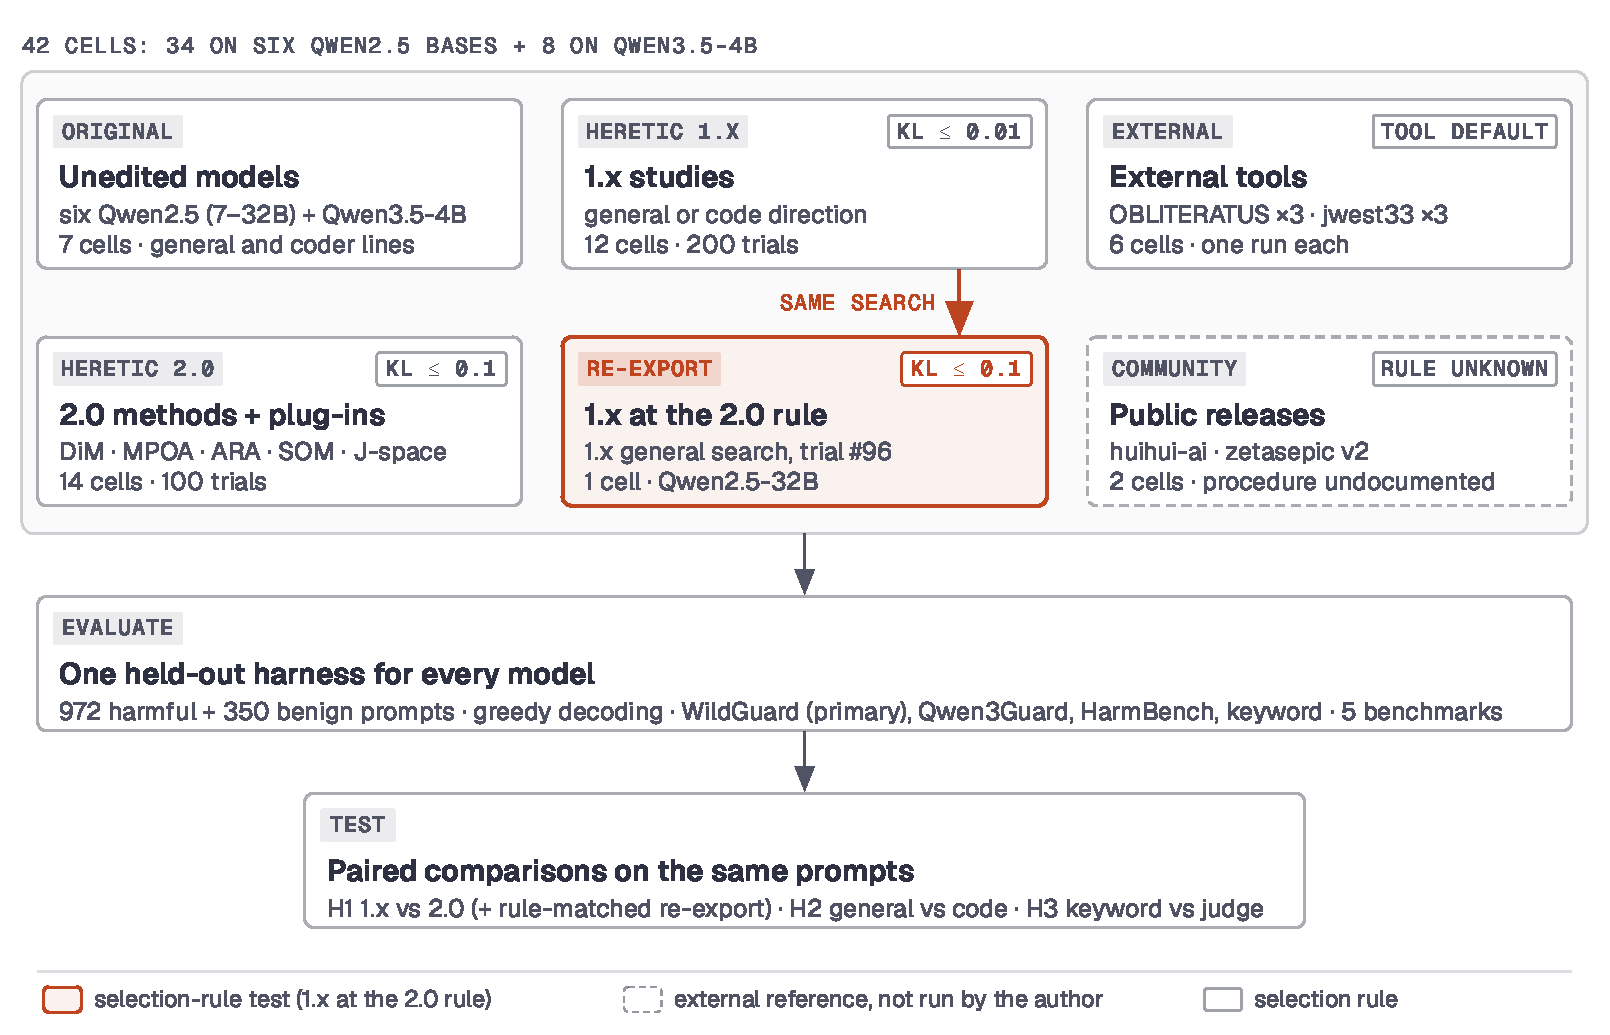
\includegraphics[width=\textwidth]{figures/fig0_study_design.pdf}
\caption{\textbf{Study design.} Six kinds of model on the same Qwen2.5 bases are evaluated with one held-out,
judge-based harness and compared with paired tests on the same prompts. The highlighted condition is the selection-cap
test: the original Heretic~1.x general study on Qwen2.5-32B re-exported at the Heretic~2.0 selection rule
(\S\ref{sec:reexport}). Community releases (dashed) were produced by others with undocumented procedures; the
external tools were run by the author with their default or recommended settings. ``Rule-matched'': both arms selected
by the same rule, not at matched divergence.}
\label{fig:design}
\end{figure*}

\subsection{Models and Conditions}
\label{sec:models}

% src (RESULTS.md "Coverage": 42 of 42 judged; scripts/supp_stats.py COMPANION set; cells.csv provenance)
All base models of the main design are Qwen2.5 instruction-tuned checkpoints \cite{qwen2024qwen25,hui2024qwen25coder}
in two lines, general (Qwen2.5-7B, -14B and -32B-Instruct) and coder (Qwen2.5-Coder-7B, -14B and -32B-Instruct), run
unquantised in bf16. Each base model is evaluated unedited (the \emph{original}) and after one or more edits
(Table~\ref{tab:conditions}, Figure~\ref{fig:design}); a model--condition combination is called a \emph{cell}. The main design has 29 cells,
all judged: the six originals, twelve Heretic~1.x models (a general and a code variant on each base model), nine
Heretic~2.0 and fork-plug-in models (five on Qwen2.5-7B, four on Qwen2.5-32B) and two community releases of
Qwen2.5-32B. Thirteen of these cells were first reported in the companion study \cite{young2026harder}: the
Qwen2.5-7B and Qwen2.5-32B originals, the nine Heretic~2.0 and fork-plug-in models and the two community releases.
Their responses and judge labels are reused here and are marked in the Source column of Table~\ref{tab:cells}. The
other 16 cells are new: the twelve 1.x models and the Qwen2.5-Coder-7B, Qwen2.5-14B, Qwen2.5-Coder-14B and
Qwen2.5-Coder-32B originals. Thirteen cells were added after the main design (\S\ref{sec:deviations}): the
Qwen2.5-32B 1.x general search re-exported at the Heretic~2.0 selection rule (\S\ref{sec:reexport}); four
external-tool cells on Qwen2.5-7B and two on Qwen3.5-4B (\S\ref{sec:external}); and, as context for the latter, the
Qwen3.5-4B original and its five seed-1 Heretic~2.0 and fork-plug-in models from the companion study, whose
responses and judge labels are reused. In total 42 cells were judged.

\begin{table*}[tbp]
\centering\small
\caption{Conditions. All Heretic edits act on the attention output projection and the MLP down-projection of each
layer. TPE = multivariate tree-structured Parzen estimator in Optuna; KL = first-token KL divergence from the
original on 100 harmless prompts (\texttt{mlabonne/harmless\_alpaca} test[:100]; 1.x code: its own benign-code
evaluation prompts); dev = development prompts whose
keyword refusals the search minimises. General direction data: \texttt{mlabonne/harmful\_behaviors} versus
\texttt{mlabonne/harmless\_alpaca}, train[:400] each; general dev set: \texttt{harmful\_behaviors} test[:100].
Fork plug-in: method from the project fork \texttt{paper33-plugins} (commit \texttt{8fd4d76}) of the companion
study, not part of the Heretic~2.0 releases. Heretic~1.x general and Heretic~2.0 DiM apply the same edit family
with different search ranges and objectives (Table~\ref{tab:h1setup}). Qwen3.5-4B cells of the 2.0 and fork configurations are seed-1 models of the companion
study, included as context for the external tools. External tools were run once at their own default or recommended
settings, without a search or a selection rule by the author (\S\ref{sec:external}).}
\label{tab:conditions}
\setlength{\tabcolsep}{4pt}
\begin{tabular}{@{}>{\raggedright\arraybackslash}p{2.25cm}>{\raggedright\arraybackslash}p{2.9cm}%
>{\raggedright\arraybackslash}p{2.75cm}>{\raggedright\arraybackslash}p{2.7cm}%
>{\raggedright\arraybackslash}p{2.55cm}>{\raggedright\arraybackslash}p{1.45cm}@{}}
\toprule
Condition & Edit & Direction data; dev set & Build and search & Selection rule & Models \\
\midrule
1.x general & rank-1 directional ablation, per-layer kernel; no projection, no row normalisation & general;
general & heretic-llm 1.4.0; TPE, 200 trials (60 random), seed~0 & fewest dev refusals at KL $\le$ 0.01 (archived
runs) & all six \\
1.x code & as 1.x general & malicious- vs benign-code prompts; 100 held-out malicious-code prompts & as 1.x general &
as 1.x general & all six \\
1.x general, KL $\le$ 0.1 & as 1.x general & as 1.x general & re-export of the archived 1.x general search
(\S\ref{sec:reexport}) & fewest dev refusals at KL $\le$ 0.1 (2.0 rule): trial \#96 & 32B \\
\midrule
2.0 DiM & rank-1 DiM ablation (same edit family as 1.x) & general; general & Heretic~2.0.0; TPE, 100 trials (30 random),
seed~1 & fewest dev refusals at KL $\le$ 0.1 (companion study) & 7B, 32B; Qwen3.5-4B \\
2.0 MPOA & projected, norm-preserving (rank 3) & as 2.0 DiM & as 2.0 DiM & as 2.0 DiM & 7B, 32B; Qwen3.5-4B \\
2.0 ARA & rank-50 LoRA per module, L-BFGS & as 2.0 DiM & as 2.0 DiM & as 2.0 DiM & 7B, 32B; Qwen3.5-4B \\
SOM (fork plug-in) & $k=4$ SOM directions, projected, norm-preserving (rank 6) & as 2.0 DiM & fork \texttt{8fd4d76}; as 2.0
DiM & as 2.0 DiM & 7B, 32B; Qwen3.5-4B \\
J-space (fork plug-in) & Jacobian-lens direction, row-normalised (rank 3) & lens direction (no contrast set);
general & fork \texttt{8fd4d76}; as 2.0 DiM & as 2.0 DiM & 7B; Qwen3.5-4B \\
\midrule
Community & not documented & -- & -- & -- & 32B \\
\midrule
OBLITERATUS: \texttt{basic}, \texttt{advanced}, \texttt{spectral\_}\allowbreak\texttt{cascade} & tool presets (\S\ref{sec:external}) &
tool's built-in 842 harmful and 842 harmless prompts & v0.1.4 (\texttt{461ff086}); preset defaults, seed~1 & none
(tool output) & 7B \\
jwest33 abliterator & all linear layers; norm-preserving, winsorised, null-space constrained & 30 harmful and 30
harmless prompts sampled from the tool's pools & commit \texttt{6ca3356e}; recommended settings, seed~1 & none
(tool output) & 7B; Qwen3.5-4B (as released; hybrid fix as sensitivity run) \\
\bottomrule
\end{tabular}
\end{table*}

% src (reexport_1x/VERSION.md: heretic-llm 1.4.0 = git v1.4.0 6ea3b8d, evidence 1-5; cells.csv adapter_sha256_ok,
%      tensors_*; reexport_1x/validation_7b/SUMMARY.json for the 7B general merge check; code-study journals
%      results/heretic/Qwen__*__code/study/*.jsonl: trial user attr n_bad_prompts = 100 in all six studies (1.4.0
%      main.py l.644: len(evaluator.bad_prompts), evaluator.py l.38: bad_evaluation_prompts); settings
%      good/bad(_evaluation)_prompts = configs/code_abliteration_data/{benign_code_prompts,malicious_code_prompts,
%      benign_code_eval,malicious_code_eval}.txt)
\paragraph{Heretic~1.x.} Rank-1 LoRA adapters \cite{hu2022lora} produced in June 2026 with Heretic~1.x
\cite{heretic2025} were available for all six base models in two variants; they were produced by the author's earlier, unpublished
code-abliteration study. The run records do not name the release,
but the key set and order of the settings record stored in every 1.x study journal, together with the search range
that the journals record for the MLP ablation weight, identify it as heretic-llm 1.4.0 (git tag \texttt{v1.4.0},
commit \texttt{6ea3b8d}); earlier revisions store a different key order and later ones a different search range
(Appendix~\ref{app:reexport}). The \emph{general} variant computes the refusal direction from the first 400
training prompts of \texttt{mlabonne/harmful\_behaviors} and \texttt{mlabonne/harmless\_alpaca}
\cite{zou2023universal,taori2023alpaca}, as Heretic does by default. The \emph{code} variant computes it from
malicious-code requests (RMCBench and MalwareBench) against benign coding prompts (MBPP), uses a held-out file of
malicious-code requests as its dev set (100 prompts, the count stored with every trial) and a file of benign coding
prompts for its KL term. The code pipeline therefore differs from the general one in its direction data, dev set
and KL prompts, not only in its direction. These four prompt files, and the script that generated them, were not archived with the
run records, so their contents and the sizes of the direction sets are unknown. Both variants ran 200 TPE trials (60 random) with
seed~0, the optimisation system prompt ``You are a helpful coding assistant.'', at most 100 generated tokens per dev
response, a list of 32 keyword markers (Heretic's default list without ``disclaimer''), and a KL target of 0.01:
the 1.x objective is a pair of minimised scores, the KL divergence (replaced, below the target, by the normalised
refusal count times the target) and the refusal count normalised by the base model's dev refusals. The 1.x build also exposed the
direction-projection and row-normalisation options that define MPOA, but the archived runs switched them off. The
released trial was chosen by the archived study's batch wrapper, not by Heretic: the fewest dev refusals among trials
with KL $\le$ 0.01, a cap met in all 12 runs. Each adapter was merged into its base model on CPU. The SHA-256 of all
12 adapters matched their manifests; for the eight 14B and 32B adapters the rebuilt merges were tensor-for-tensor
identical to the archived merges, and for the four 7B adapters no tensor hashes of the archived merges had been
recorded (Appendix~\ref{app:checks}).

Heretic's directional ablation, in both versions, differs from the edit of Arditi et al.\ \cite{arditi2024refusal},
which orthogonalises every residual writer, including the embedding, against one direction at full strength: Heretic
edits only the attention output and MLP down-projections, with a per-layer weight kernel (a maximum weight, its
position and a minimum weight at a given distance) and either one direction interpolated between two layers'
directions or a separate direction per layer, all chosen by the search.

\paragraph{Heretic~2.0 and fork plug-ins.} The Heretic~2.0 models are the seed-1 models of the companion study
\cite{young2026harder}: DiM (a difference-in-means direction \cite{arditi2024refusal} applied with Heretic's
per-layer weight kernel), MPOA \cite{lai2024projected,lai2025mpoa} and ARA
\cite{weidmann2026ara}, which are built into Heretic~2.0.0 (upstream commit \texttt{0db5c31}), on Qwen2.5-32B and
Qwen2.5-7B. SOM \cite{piras2025som} (on both models) and J-space ablation \cite{sekinal2026jspace} (on Qwen2.5-7B
only) are plug-ins of the companion study's project fork (branch \texttt{paper33-plugins}, commit \texttt{8fd4d76});
they are not part of any Heretic~2.0 release. SOM ports the proof of concept of Heretic pull request~\#196, and
J-space bakes directions from the \texttt{jspace-refusal} code into the weights with Heretic's row-normalised
directional ablation instead of the reference forward hook. All Qwen2.5-7B runs, including DiM, MPOA and ARA, ran
from the fork; \texttt{git diff 0db5c31 8fd4d76} shows that the fork only adds files (the SOM and
precomputed-direction modifiers and their tests) and configuration entries, without changing any line of an existing
source file, so the built-in methods are identical to \texttt{0db5c31}. All used the general direction data
and dev set, 100 TPE trials (30 random) with seed~1, Heretic~2.0's default system prompt ``You are a helpful
assistant.'', its 33 default keyword markers (the 1.x list plus ``disclaimer''), KL as a plain minimised objective,
and the companion study's selection rule: the fewest dev refusals among trials with KL $\le$ 0.1, ties broken by
lower KL. The companion study's seed-1 models of the same five configurations on Qwen3.5-4B serve only as context
for the external-tool cells on that model; they enter no test of H1--H3.

% src (tab:h1setup rows: cells.csv dev_refusals/dev_kl; RESULTS.md "Dev set at matched KL caps": 1x_general 32B
%      <=0.1 -> 50 (0.064); dim 32B selected 89 @ 0.0175; 2026-11-08 search-range and selected-weight rows:
%      analysis/revision_20261108/search_space.csv (journal distributions; selected_value of mlp.down_proj.max_weight:
%      32B #84 0.9115, #96 1.0019, DiM #62 1.2133; 7B #193 1.1455, DiM #36 1.1863))
\begin{table}[tbp]
\centering\small
\caption{Setup of the like-for-like contrast (H1). Both arms apply the same edit family with the same direction
data, dev prompts and KL prompts. Search ranges are those recorded in each search's Optuna journal ($L$ = index of
the last layer; 63 for Qwen2.5-32B, 27 for Qwen2.5-7B); they agree with the source of heretic-llm~1.4.0 and of
Heretic \texttt{0db5c31}. The only range that differs is that of the MLP maximum weight; no selected or re-exported
trial used a value below 0.8. Released trial: dev keyword refusals of 100 (dev KL), each counted under its own arm's
system prompt and marker list. The last row gives the trial that the 2.0 rule selects from each search on
Qwen2.5-32B; the 1.x trial was re-exported and evaluated (\S\ref{sec:reexport}).}
\label{tab:h1setup}
\setlength{\tabcolsep}{4pt}
\begin{tabular}{@{}>{\raggedright\arraybackslash}p{3.0cm}>{\raggedright\arraybackslash}p{5.2cm}%
>{\raggedright\arraybackslash}p{5.2cm}@{}}
\toprule
Setting & Heretic~1.x general (archived runs) & Heretic~2.0 DiM (companion study) \\
\midrule
Edit & rank-1 directional ablation, no projection, no row normalisation & same \\
Direction & global (interpolated) or per layer; index in $[0.4L, 0.9L]$ & same \\
Attention max.\ weight & $[0.8, 1.5]$ & same \\
MLP max.\ weight & $[0.8, 1.5]$ & $[-0.25, 1.5]$, clamped at 0 \\
Weight kernel & position $[0.6L, L]$; min.\ weight $[0, 1]\times$max.; distance $[1, 0.6L]$ & same \\
Selected MLP max.\ weight & 32B: 0.91 (\#84), 1.00 (\#96); 7B: 1.15 & 32B: 1.21; 7B: 1.19 \\
Direction data; dev; KL prompts & general; general; \texttt{harmless\_alpaca} test[:100] & same \\
Build & heretic-llm 1.4.0 (\texttt{6ea3b8d}) & v2.0.0 (\texttt{0db5c31}); Qwen2.5-7B: fork
\texttt{8fd4d76} \\
Trials (random), seed & 200 (60), seed~0 & 100 (30), seed~1 \\
Optimisation system prompt & ``You are a helpful coding assistant.'' & ``You are a helpful assistant.'' \\
Keyword markers (dev) & 32 & 33 (adds ``disclaimer'') \\
Objective (both minimised) & KL with target 0.01 (below it: scaled refusal score); refusals / base refusals &
keyword refusal rate; KL, no target \\
Selection rule & fewest dev refusals, KL $\le$ 0.01 & fewest dev refusals, KL $\le$ 0.1 \\
Released trial, Qwen2.5-32B & 89 (0.006) & 89 (0.018) \\
Released trial, Qwen2.5-7B & 67 (0.005) & 55 (0.078) \\
Trial at the 2.0 rule, Qwen2.5-32B & 50 (0.064), trial \#96, re-exported & 89 (0.018), the released trial \\
\bottomrule
\end{tabular}
\end{table}

\paragraph{Community releases.} Two public abliterations of Qwen2.5-32B-Instruct were evaluated as released:
\path{huihui-ai/Qwen2.5-32B-Instruct-abliterated} (revision \texttt{546fc405}) \cite{huihui2025qwen32b} and
\path{zetasepic/Qwen2.5-32B-Instruct-abliterated-v2} (revision \texttt{5894fbf0}) \cite{zetasepic2025qwen32b}.
Their procedures, prompt sets and selection rules are not documented.

\subsection{Selection-Cap Re-Export}
\label{sec:reexport}

% src (reexport_1x/VERSION.md; reexport_1x/run_on_rtx.sh header (rule: KL <= 0.1, fewest dev refusals, ties -> lower
%      KL; general #96 50/100 KL 0.0642, code #134 2/100 KL 0.0717); results_rtx/qwen2.5-32b__heretic1x-general-kl0.1/
%      PROVENANCE.json (journal_sha256 bf60f054..., settings_roundtrip_identical, base_model_revision 5ede1c97,
%      journal_values 50 @ 0.06423, reevaluated 51 @ 0.06367, n_edited_modules 80, verdict PASS);
%      results_rtx/trial84_validation_records/PROVENANCE.json (validation.adapter: 62/62, min_direction_cosine
%      0.9999876; reevaluated 90 @ 0.00553; reevaluated_original_adapter_here 90 @ 0.00535; journal 89 @ 0.00592);
%      results_rtx/reexport_1x.log l.246-248 (merged 709/771 identical, max_abs_diff 0.0078125, PASS))
The two arms of the like-for-like contrast were released under different selection caps (dev KL $\le$ 0.01 for
1.x, $\le$ 0.1 for 2.0). To separate the cap from the version, the archived Heretic~1.x general search on
Qwen2.5-32B was re-exported at the 2.0 rule. The re-export used heretic-llm 1.4.0 with the dependency versions
locked by that release (transformers 5.6.2, PEFT 0.19.1, Optuna 4.8.0) and PyTorch 2.14.1, because the PyTorch
version of the original runs was not recorded. A re-export script loaded the original study journal, checked that its stored
settings pass unchanged through the 1.4.0 settings class (only the local model path and the automatic batch size
were overridden), recomputed the refusal directions with the 1.4.0 code from the same prompts, rebuilt the rank-1
adapter of the requested trial from its stored parameters, re-evaluated it on the 100 dev and 100 KL prompts and
merged it into the base model (revision \texttt{5ede1c97}). The trial selected by the 2.0 rule (fewest dev
refusals among trials with dev KL $\le$ 0.1, ties broken by lower KL) was trial~\#96: 50 of 100 dev refusals at a
dev KL of 0.064 in the journal, and 51 at 0.064 on re-evaluation. The released trial~\#84 had 89 at 0.006.

Before trial~\#96 was used, the same script re-exported the released trial~\#84 and compared it with the archived
adapter; a failure of this gate would have stopped the run before trial~\#96 was exported. The re-exported and
archived adapters edited the same 62 modules; their weights were not bit-identical, but the minimum direction cosine
between corresponding modules was 0.99999. In the merged models 709 of 771 tensors were bit-identical, and the other
62 differed by at most 0.0078 in absolute value. The re-exported adapter kept 90 dev refusals, the archived adapter
evaluated in the same run 90 and the journal 89. The re-export was therefore accepted as numerically equivalent to the
original, and the trial~\#96 model was evaluated with the same harness as every other cell. The 1.x code search could
not be re-exported, because its four prompt files (the malicious- and benign-code direction prompts and the two
evaluation files) were never copied from the archived study's repository; without them its refusal directions cannot
be recomputed. Only the general variant on Qwen2.5-32B therefore has a KL $\le$ 0.1 cell. Provenance and the
acceptance criteria are given in Appendix~\ref{app:reexport}.

\subsection{External Tools}
\label{sec:external}

% src (/data/heretic_2/models/external/*/PROVENANCE.json: commit, preset, preset_definition, resolved_config,
%      runtime_patches, hybrid_detection, seed, base_revision, prompt_sets, tool_reported_metrics; cells.csv ext_*;
%      tools_ext/README.md (preset mapping, som not shipped, Qwen3.5 contract, CLI hybrid-detection omission))
Two external abliteration tools were run by the author with each tool's documented default or recommended settings
and evaluated with the same harness as the Heretic cells. No search over their settings was made and their outputs
were not selected by dev KL; each tool contributes the single model it produced. Every run used seed~1, bf16 weights
and the base revisions of the Heretic cells (Qwen2.5-7B-Instruct \texttt{a09a3545}, Qwen3.5-4B \texttt{851bf6e8}).
The tools' code was used from clean checkouts; every deviation is a named runtime patch in a wrapper, recorded in
each output's provenance record (Appendix~\ref{app:external}).

OBLITERATUS \cite{obliteratus2026} v0.1.4 (commit \texttt{461ff086}) was run with three presets on Qwen2.5-7B,
\texttt{basic}, \texttt{advanced} and \texttt{spectral\_cascade}, through the tool's Python pipeline with every
preset default (bf16 instead of the command-line default float16) and no runtime patch. All presets compute
directions from the tool's built-in list of 842 harmful and 842 harmless prompts, of which one harmful prompt is a
held-out JailbreakBench prompt that also belongs to the 44 AdvBench-overlap prompts (\S\ref{sec:measures}).
\texttt{basic} is the preset closest to Arditi et al.\ (one difference-in-means direction, no norm preservation),
but it is not a reproduction of that method or of Heretic's DiM: it feeds the prompts without the chat template and
edits only the layers chosen by its knee-based heuristic (ten layers on Qwen2.5-7B), whereas Arditi et al.\
orthogonalise every residual writer. \texttt{advanced} removes four SVD directions with norm preservation and
regularisation (seven layers); \texttt{spectral\_cascade} removes six whitened-SVD directions, extracted with an
additional jailbreak contrast, with iterative refinement and a frequency decomposition of the refusal signal across
layers (16 layers). The \texttt{som} preset is listed in v0.1.4 but its
direction module is not shipped, so the preset fails by design and is reported as not available. OBLITERATUS v0.1.4
does not support Qwen3.5-4B: for the hybrid-attention Qwen3.5 architecture its validation step accepts only one
larger Qwen model and stops before any weight is modified, so no OBLITERATUS model exists for Qwen3.5-4B and that
cell is reported as not supported.

The jwest33 abliterator \cite{jwest33abliterator} (commit \texttt{6ca3356e}) was run through its own batch command
line with the settings that its interactive mode labels as recommended (``Recommended standard'' for dense models,
``Recommended for hybrid model'' for Qwen3.5; both translate to the same batch flags): winsorisation and the
null-space constraint, with norm preservation, projected refusal directions, all linear layers of the language model
and the other values at their defaults. The tool samples 30 harmful and 30 harmless prompts from its default pools
(5{,}000 each) and filters the harmful ones by a log-likelihood refusal test. Three wrapper measures leave the
tool's code unchanged: the prompt files, deleted from the repository after commit \texttt{a2a7940}, are supplied
from that commit; the tool's unseeded prompt sampling is seeded; and the prompts actually used are recorded. All
three jwest33 runs used the same 30 harmful and 30 harmless prompts. One of the harmful prompts is a held-out
JailbreakBench prompt that also belongs to the 44 AdvBench-overlap prompts, so the analysis without those prompts
excludes it. The tool's known behaviour on square residual writers, which it projects on the input side (the
$3{,}584\times3{,}584$ attention output projection of Qwen2.5-7B), was left uncorrected.

The tool's library entry point detects hybrid architectures and, for them, restricts direction extraction to the
full-attention layers and the linear-attention layer before each and down-weights the linear-attention layers; its
batch command line omits that detection, so the documented default hybrid strategy has no effect there. On
Qwen3.5-4B the primary cell is the tool as released (no runtime patch). A second run with a runtime patch that sets
the detected architecture information before direction extraction, as the library entry point does, is reported as
a sensitivity analysis; the as-released run was designated primary before it was generated. On Qwen2.5-7B, which the
tool detects as non-hybrid, the same patch was active but changes nothing, so the Qwen2.5-7B cell is in effect the
tool as released. The Qwen3.5-4B cells lie outside the Qwen2.5 design; they are compared with the Qwen3.5-4B
original and its five companion-study models (\S\ref{sec:models}).

% src (PROVENANCE.json tool_reported_metrics: OBLITERATUS refusal_rate 0.833/0.400/0.033, verify_sample_size 30;
%      jwest33: filter settings only; assemble_p30.py l.553-554)
Both tools check their output on their own prompts. OBLITERATUS reports a refusal rate on a verification sample of 30
prompts from its built-in harmful list, together with perplexity, coherence and a sequence-level KL divergence;
jwest33's batch run reports its filter settings but no refusal rate. These self-reports use other prompts, markers
and generation lengths than the held-out harness and are not comparable with its measures; the OBLITERATUS refusal
rate is used only to check whether the tool's own assessment agrees in direction with the judged result.

\subsection{Measures}
\label{sec:measures}

% src (RESULTS.md "Coverage" WG N/A column and "Anomalies and checks": 2 harmful (qwen2.5-32b__base,
%      qwen2.5-7b__obliteratus-advanced), 1 benign (qwen2.5-7b__som) of 42 x 972 = 40,824 / 42 x 350 = 14,700;
%      judge revisions; degenerate() in paper-33 scripts/bench/score_refusals.py)
\paragraph{Held-out refusal.} One greedy response (at most 512 new tokens, the model's chat template, system
prompt ``You are a helpful assistant.'') to each of 1{,}322 held-out prompts was generated with vLLM
\cite{kwon2023efficient}. The 972 harmful prompts comprise JailbreakBench harmful (100), XSTest unsafe (200),
StrongREJECT (313), HarmBench standard (159) and a code-as-weapon sample (200; malicious-code requests whose
answer would be working attack code)
\cite{chao2024jailbreakbench,rottger2024xstest,souly2024strongreject,mazeika2024harmbench,young2026code}; the 350
benign prompts are JailbreakBench benign (100) and XSTest safe (250). The set is held out from search and selection
except for 44 harmful prompts that exactly (36) or approximately (8) match a prompt of \texttt{harmful\_behaviors},
which are analysed with and without; 41 code-as-weapon prompts come from RMCBench or MalwareBench, the sources of
the 1.x code direction, and are likewise analysed with and without for H2. The \emph{primary outcome} is the
WildGuard \cite{han2024wildguard} refusal label of each harmful response (residual refusal); responses without a
WildGuard label (2 of 40{,}824 harmful and 1 of 14{,}700 benign responses) are dropped pairwise. Secondary refusal
measures are Heretic~2.0's 33 default keyword markers on the full response and on its first 256 tokens, and the
refusal label of Qwen3Guard-Gen-8B \cite{zhao2025qwen3guard}; harmful compliance is the HarmBench classifier's label
\cite{mazeika2024harmbench}; over-refusal is the WildGuard refusal rate on the benign prompts. A response that reached
the 512-token limit is called \emph{capped}. A response is flagged \emph{degenerate} by the harness's heuristic
\cite{young2026harder} if it is empty, if more than half of its word 4-grams repeat or fewer than 15\% of its words
are distinct (responses of at least 20 words), if it contains a run of more than 40 identical characters (code and
markdown separators excepted) or if more than 20\% of its characters are non-printable; degenerate responses keep
their judge labels and are reported as a rate. Judge revisions were identical for every cell (WildGuard
\texttt{cbba4823}, Qwen3Guard \texttt{4505cb1a}, HarmBench classifier \texttt{bda70534}).

\paragraph{Capability and distribution shift.} Five benchmarks ran with lm-evaluation-harness 0.4.13
\cite{gao2024language} on vLLM 0.33.0 with greedy decoding: MMLU-Pro (1{,}000 items) \cite{wang2024mmlupro},
GSM8K (500) \cite{cobbe2021training}, IFEval (541) \cite{zhou2023instruction}, HumanEval (164)
\cite{chen2021evaluating} and MBPP (500) \cite{austin2021program}. Distribution shift on held-out data is the
\emph{teacher-forced (TF) divergence}: the token-averaged $\log p_{\mathrm{orig}}(y)-\log p_{\mathrm{mod}}(y)$ over
the original model's own greedy responses $y$ to the 350 benign held-out prompts. The \emph{dev KL} is the
first-token KL divergence that the search recorded for a trial on its KL prompts (\texttt{harmless\_alpaca}
test[:100]; for the 1.x code variant, its own benign-code evaluation prompts). The \emph{selection
rule} picks the released trial from a search, its \emph{selection cap} is the dev-KL threshold of that rule, and
the \emph{search budget} is the number of trials. ``Divergence'' without qualification is not used for dev KL. The
external tools have no dev KL; the divergence figures they report themselves (Appendix~\ref{app:external}) are not
used in the analysis.

\subsection{Procedure}
\label{sec:procedure}

% src (cells.csv ref_dir/gen_dirs/cap_dir: results/bench-4090/* for the new 7B, Coder-7B and Qwen3.5-4B jwest33
%      cells; eval.log host=4090-omarchy, "NVIDIA GeForce RTX 4090"; summary.json judge_revisions;
%      runs/mc-rtx-1/results/bench/qwen2.5-32b__heretic1x-general-kl0.1; external PROVENANCE.json gpu RTX 4090;
%      reexport PROVENANCE.json environment.gpus RTX PRO 6000 Blackwell Server Edition)
% src (2026-11-08 re-review NEW-3): 33_.../runs/mc-h200-1/runs/qwen2.5-32b__{dim,mpoa,som,ara}__core-s1/meta.txt
%      ("torch 2.14.1+cu130 NVIDIA H200 NVL", heretic 0db5c31); revision_20261108/search_cost.csv (7B 2.0/fork searches
%      RTX 4090 from meta.txt; 1.x searches gpu "not recorded")
The 14B and 32B models, including the KL $\le$ 0.1 re-export, and the judges of all companion-study cells ran on one
NVIDIA RTX PRO 6000 (96 GB); the re-export itself was computed on an RTX PRO 6000 of the same type. The companion
study's Qwen2.5-7B and Qwen3.5-4B models were generated and benchmarked on an RTX 4090 and judged on the RTX PRO
6000. The new Qwen2.5-7B and Qwen2.5-Coder-7B cells (1.x and external tools) and the two jwest33 Qwen3.5-4B cells
were generated, benchmarked and judged on the RTX 4090 with the same judge revisions; the external tools also ran
there. The companion study's Heretic~2.0 and fork searches ran on one NVIDIA H200 NVL (Qwen2.5-32B) and on the
RTX 4090 (Qwen2.5-7B) \cite{young2026harder}; the GPUs of the archived 1.x searches were not recorded. Within each
base model, all cells used the same prompts, decoding settings, reference responses for TF
divergence and judges, with one exception. The Qwen2.5-32B original was evaluated in two earlier harness runs
(capability; held-out generation and teacher forcing) whose evaluation-script revision differs from that of its
edited models; these runs did not apply the output post-processing of later runs (mapping the SentencePiece
character U+2581 to a space; the original's outputs contain none), and its MBPP run predates the patched answer
extractor, so its per-item MBPP samples are unpatched and only its MBPP summary score was rescored from the logged
outputs \cite{young2026harder}. Data checks are listed in Appendix~\ref{app:checks}.

\subsection{Data Analysis}
\label{sec:stats}

% src (2026-11-08): sigma 9.15 [6.40, 16.07], SD_diff 12.95, threshold 25.89 [18.09, 45.44], equal-batch threshold 20.35:
%   analysis/revision_20261108/seednoise_derivation.csv (recomputed from paper-33 results/analysis/seednoise_seed_pairs.csv;
%   identical to paper-33 seednoise_sigma.csv and review_sel_seed_sigma.csv); equivalence margin and TOST:
%   revision_20261108/capability_equivalence.csv; clustered correlations: revision_20261108/correlations_clustered.csv.
% src (2026-11-08 re-review S7): revision_20261108/s7_correlations.csv (n_boot_degenerate 0 for all; within_model_p_scipy
%   0.0045 / 0.19 / 0.0026; within_model_p_df_adjusted 0.013 / 0.218 / 0.0088 for tf, dev_kl general, capability).
% src (tests_refusal.csv n_in_family by family: vs_base 23, h1_1x_vs_2.0 18, h2_general_vs_code 6,
%      within_model_pairs 76, kw_vs_judge 29; vs_base_added 12, h1_kl_matched 4, kl_cap_1x 1, external_vs_heretic 38,
%      external_sensitivity 1, kw_vs_judge_added 13; tests_capability.csv family original_design 23 cells x 5,
%      added 12 cells x 5; assemble_p30.py correlations(): original design only)
Rates carry Wilson 95\% intervals \cite{wilson1927probable}. Two models evaluated on the same prompts are compared
by the paired difference in rates with Newcombe's hybrid score interval \cite{newcombe1998improved} and the exact
McNemar test \cite{mcnemar1947note}, a prompt-level paired comparison \cite{miller2024adding}; each test therefore
compares two released checkpoints on these prompts and conditions on their searches. Holm's procedure
\cite{holm1979simple} controls each family of tests at two-sided $\alpha=0.05$, separately for each refusal measure
and prompt subset. The families of the main design are: each edited model versus its original (23 tests); the
1.x-versus-2.0 family, each 1.x variant versus each 2.0 method or fork plug-in on the same base model (18 tests, 8
on Qwen2.5-32B and 10 on Qwen2.5-7B); H2, 1.x general versus 1.x code per model (6 tests per subset); all pairs of
cells within a model (76 pairs, exploratory); and H3, keyword versus WildGuard on the same responses of each cell
(29 tests). The primary H1 test is the 1.x general versus 2.0 DiM contrast on each base model; it is adjusted within
the whole 1.x-versus-2.0 family, which is conservative for it, and the other contrasts of that family describe the
additional configurations. The added cells form separate families, so that the main-design results do not change
with their addition: each added cell versus its original (12 tests); the KL $\le$ 0.1 re-export versus the four
2.0 and fork configurations on Qwen2.5-32B (4 tests); the KL $\le$ 0.1 versus the KL $\le$ 0.01 export of the same
search (1 test, unadjusted); each external-tool cell versus each Heretic cell on the same base model (38 tests);
jwest33 as released versus with the hybrid fix (1 test, unadjusted); and keyword versus WildGuard for the added
cells (13 tests). Capability is compared per item with the same paired interval and test, Holm-adjusted over the
115 cell--benchmark tests of the main design and separately over the 60 of the added cells; the mean change over
the five benchmarks carries a normal interval from the per-benchmark paired variances. MBPP changes on the
Qwen2.5-32B original use an unpaired normal test on the summary scores (\S\ref{sec:procedure}). Whether a
capability change is negligible is assessed with two one-sided tests against an equivalence margin of $\pm$2~pp on the
mean of the five benchmarks (equivalence when the 90\% interval lies inside the margin); the margin was chosen after
the results were known, and the minimum change detectable with 80\% power is reported beside it. Associations across
edited models are Spearman correlations over the 23 edited models of the main design. Because these models are
clustered in six base models, their intervals come from a bootstrap that resamples base models with all their cells
(4{,}000 resamples, percentile intervals; a resample in which either variable was constant or fewer than four cells
remained would have been skipped, and none was), and each correlation is also reported for values centred within each
base model, the analogue of base-model fixed effects. The $p$-value of a within-base correlation is that of the
Spearman test on the centred values of the base models with at least two cells (t approximation with $n-2$ degrees of
freedom); it does not deduct the degrees of freedom used by centring and is therefore somewhat liberal (with that
deduction the within-base $p$-values of \S\ref{sec:res-tradeoff} become 0.013 for TF divergence, 0.22 for dev KL and 0.009 for capability). The original
percentile bootstrap over cells is kept in the analysis records. The association
with dev KL is reported only for the cells scored on the general dev protocol, because the code variants measure dev
KL on other prompts. All cross-model correlations are exploratory. Within a base model, the association of residual refusal with TF
divergence is a Spearman correlation with an exact permutation $p$-value. To separate search quality from the
selection rule, the fewest dev refusals reachable at dev-KL caps of 0.01 to 0.5 were read from the optimisation
records: the Pareto fronts of the 1.x runs and all trials of the 2.0 runs (the fewest refusals under a cap is always
attained on the Pareto front, so the two sources give the same values). The same records give each arm's fewest dev
refusals at the realised dev KL of the other arm's released trial, a comparison at matched dev divergence on the dev
prompts only.

\paragraph{Search-level decision rule.} The hypotheses concern versions, settings and pipelines, so their unit of
replication is the search, and each configuration contributed one search per base model. A prompt-level test
quantifies only prompt-sampling noise for two fixed checkpoints. Search-to-search variation is taken from the seed
replicates of the companion study: the run-to-run standard deviation of one cell's residual refusal, $\sigma = 9.2$~pp
[6.4, 16.1], gives a standard deviation of a difference between two independently optimised cells of
$\sqrt{2}\,\sigma = 12.9$~pp and a threshold of two such standard deviations, 25.9~pp with a 95\% interval of
[18.1, 45.4] (Appendix~\ref{app:seednoise}). A contrast between two searches supports a hypothesis at the search
level only if it is Holm-significant and its absolute size exceeds the upper limit of that interval (45.4~pp). A
Holm-significant contrast of smaller size is reported as ``significant for these checkpoints; search-level evidence
inconclusive''; a contrast that is not Holm-significant does not support the hypothesis. The point threshold and the
threshold without the three seed-2 runs that used a smaller batch size (20.4~pp) are reported as sensitivity
readings. Contrasts between two exports of the same search (the selection-cap contrast) involve no search-to-search
variation and are decided by the prompt-level test, but they describe one search. Keyword-versus-judge contrasts (H3)
compare labels of identical responses and are decided by the prompt-level test. External-tool cells are single runs at
uncontrolled divergence; their contrasts are reported descriptively, with the divergence of each cell, and are not
used to rank tools. Analyses used Python 3.12.15 with pandas
3.1.1, NumPy 2.5.4, SciPy 1.18.1 and statsmodels 0.15.0 \cite{seabold2010statsmodels}.

\subsection{Ethics, Preregistration and Deviations}
\label{sec:deviations}

No human participants were involved. The study was not preregistered; the hypotheses were written after the
Heretic~2.0 cells had been analysed for the companion study. H1 originally predicted that every Heretic~2.0 method
would leave less residual refusal than Heretic~1.x; after an internal review it was narrowed to the like-for-like
contrast (1.x general versus 2.0 DiM), because the other methods change the edit as well as the setup and two of
them are fork plug-ins. The narrowing was made before the 7B 1.x cells were judged, but after the 32B results were
known. Three analyses were added after the main results were known and are reported in their own test families:
the KL $\le$ 0.1 re-export (\S\ref{sec:reexport}), specified as a check of the selection-cap explanation after
the Qwen2.5-32B H1 result was known; the external-tool cells; and the Qwen3.5-4B cells of the companion study as context for jwest33 on
that model. The comparison set deviates from the plan in four ways. First, Heretic~2.0 methods were not run on
Qwen2.5-14B or the coder models, so on those models 1.x is compared with the original only. Second, the selection
cap was tested on one search only, the 1.x general search on Qwen2.5-32B; the code search could not be re-exported
(\S\ref{sec:reexport}), and no Qwen2.5-7B trial at the 2.0 rule was evaluated on the held-out prompts. Third, of the external tools, OBLITERATUS contributes
three presets on Qwen2.5-7B only (its \texttt{som} preset lacks its direction module and it does not support
Qwen3.5-4B), and jwest33 contributes one Qwen2.5-7B cell and, outside the Qwen2.5 design, a primary and a
sensitivity cell on Qwen3.5-4B. Fourth, ErisForge, llm-abliteration \cite{jimplus_llmabliteration} and FailSpy were not re-run and are represented
only by the earlier comparison \cite{young2025comparative}, which labelled llm-abliteration as DECCP; DECCP is a
separate tool \cite{lin2024deccp}. In response to internal review, the following analyses of existing records were
added after all results were known: the search-level decision rule and the derivation of the seed-noise threshold
(Appendix~\ref{app:seednoise}), the dev-set comparison at matched dev KL, the search ranges and costs read from the
optimisation journals, the cosines between the general and code directions, the correlations with clustering by base
model, and the capability equivalence tests, whose margin was chosen after the capability results were known. No new
model was generated or evaluated for them.

% =====================================================================
% 4 RESULTS (describe only). Every number: analysis/RESULTS.md, cells.csv, cell_rates.csv, tests_refusal.csv,
% tests_capability.csv, correlations.csv, dev_matched_kl.csv, rank_flips.csv (assemble_p30.py, re-run 2026-11-06
% 22:47Z); supplementary statistics as computed by scripts/supp_stats.py.
% Seed-noise threshold quoted from paper 33: 33_2611_does_refusal_removal_get_harder/results/analysis/
% seednoise_summary.md (2 x SD_diff = 25.9 pp [18.1, 45.4]).
% Revised 2026-11-06: new 1.x cells lead; H1 = 1.x general vs 2.0 DiM; other configurations additional;
% H2 wording and figure caption corrected (no model showed the predicted crossover); H3 adds keyword-256;
% efficiency claim restricted to within-model evidence; selection-cap section labelled exploratory and suggestive.
% Revised 2026-11-06 (pm): 7B 1.x cells judged (H1 7B primary, H2 six models); KL <= 0.1 re-export answers the
% selection-cap question (families h1_kl_matched, kl_cap_1x); external tools (families vs_base_added,
% external_vs_heretic, external_sensitivity, kw_vs_judge_added). supp_stats.py was restricted to the 29
% original-design cells (as correlations.csv is) and re-run at 15:03 on the current analysis outputs; the supp_stats
% numbers below (within-model Spearman, keyword-256 counts, capped shares, H1 over-refusal by judge) match
% analysis/supp_stats.csv (checked 2026-11-06, integration pass).
% =====================================================================
\section{Results}
\label{sec:results}

% src (RESULTS.md "Coverage": 42 of 42 judged; "Anomalies and checks"; cells.csv wg_rate - wg_excl_adv_rate:
%      max 1.95 pp (qwen2.5-32b__dim), median 1.08 pp over the 29 main-design cells, 0.82 pp over all 42;
%      tests_refusal.csv harmful_all vs harmful_excl_advbench sig_holm: no change in vs_base, h1_1x_vs_2.0,
%      h1_kl_matched, kl_cap_1x, vs_base_added, external_sensitivity; external_vs_heretic: obliteratus-advanced vs
%      heretic1x-general (wg -4.6 [-7.7,-1.6] p=0.017 -> -3.1 [-6.2,-0.1] p=0.154) and three Qwen3Guard decisions)
The study asked which tool, version and method removes refusal best at the least capability cost when refusal is
judged on held-out prompts. Results are reported for the 29 cells of the main design (Table~\ref{tab:cells}) and
for the 13 added cells: the Qwen2.5-32B 1.x general search re-exported at the 2.0 selection rule
(\S\ref{sec:res-kl}, Table~\ref{tab:h1}) and the external tools with the Qwen3.5-4B context cells
(\S\ref{sec:res-external}, Table~\ref{tab:external}). All 42 cells passed the data checks
(Appendix~\ref{app:checks}). Excluding the 44 AdvBench-overlap prompts changed residual refusal by at most 1.95~pp
(median 1.08~pp in the main design) and left every edited-versus-original, 1.x-versus-2.0 and KL-matched decision
unchanged; among the external-tool contrasts it changed one WildGuard decision (\S\ref{sec:res-external}).

\begin{table*}[tbp]
\centering\footnotesize
\caption{Held-out results per cell of the main design and of the KL $\le$ 0.1 re-export ($^{\S}$, added after the
main design; also Table~\ref{tab:h1}b); the external-tool cells and the Qwen3.5-4B context are in
Table~\ref{tab:external}. Source: ``new'' = evaluated for this study; \cite{young2026harder} =
first reported in the companion study (responses and judge labels reused). WildGuard refusal: share of the 972
harmful prompts whose response WildGuard labels a refusal (Wilson 95\% CI). Change: paired difference from the same
model's original ($p_\mathrm{Holm}<0.001$ for 22 of the 23 changes of the main design; the exception is 1.x code on
Qwen2.5-7B, $p_\mathrm{Holm}=0.22$; the $^{\S}$ cell is tested in the separate family of added cells,
$p_\mathrm{Holm}<0.001$; for Qwen2.5-32B paired over the 971 prompts labelled in both models). Keyword: any of
Heretic~2.0's 33 default markers in the full response / in its first 256 tokens. HarmBench harmful: harmful
compliance by the HarmBench classifier. Over-refusal: WildGuard refusal on the 350 benign prompts. Capability
$\Delta$: change of the mean of the five benchmarks (pp). TF div.: teacher-forced divergence from the original on
the benign prompts (nats per token). SOM and J-space are plug-ins of the companion study's project fork, not part of
Heretic~2.0. The Qwen2.5-32B original was evaluated with an earlier harness revision (\S\ref{sec:procedure}).}
\label{tab:cells}
\setlength{\tabcolsep}{3.5pt}
\resizebox{\textwidth}{!}{\begin{tabular}{@{}lllrrrrrrrr@{}}
\toprule
Model & Condition & Source & \multicolumn{2}{c}{WildGuard refusal, harmful (\%)} & Change vs.\ & Keyword (\%) & HarmBench & Over-refusal & Capability & TF div. \\
 & & & rate & 95\% CI & original (pp) & full / 256 tok. & harmful (\%) & benign (\%) & $\Delta$ (pp) & (nats/tok.) \\
\midrule
Qwen2.5-7B & Original & \cite{young2026harder} & 72.1 & [69.2, 74.8] & -- & 75.8 / 74.5 & 23.3 & 4.3 & -- & -- \\
 & 1.x general & new & 39.6 & [36.6, 42.7] & $-$32.5 & 45.8 / 43.4 & 45.6 & 1.1 & $-$0.36 & 0.009 \\
 & 1.x code & new & 71.2 & [68.3, 74.0] & $-$0.9$^{\mathrm{ns}}$ & 71.9 / 71.4 & 25.5 & 5.1 & +0.80 & 0.075 \\
 & 2.0 DiM & \cite{young2026harder} & 20.6 & [18.2, 23.2] & $-$51.5 & 40.1 / 37.8 & 64.0 & 0.3 & +0.23 & 0.019 \\
 & 2.0 MPOA & \cite{young2026harder} & 13.8 & [11.8, 16.1] & $-$58.3 & 23.7 / 20.5 & 71.5 & 0.3 & $-$0.23 & 0.018 \\
 & SOM (fork plug-in) & \cite{young2026harder} & 12.2 & [10.3, 14.5] & $-$59.9 & 22.4 / 17.9 & 73.1 & 0.0 & $-$0.33 & 0.026 \\
 & J-space (fork plug-in) & \cite{young2026harder} & 52.6 & [49.4, 55.7] & $-$19.5 & 53.6 / 51.7 & 36.3 & 1.1 & +0.86 & 0.009 \\
 & 2.0 ARA & \cite{young2026harder} & 4.7 & [3.6, 6.3] & $-$67.4 & 16.6 / 11.0 & 79.0 & 0.0 & +0.48 & 0.048 \\
\addlinespace[2pt]
Qwen2.5-Coder-7B & Original & new & 83.2 & [80.8, 85.4] & -- & 83.6 / 83.5 & 15.4 & 22.6 & -- & -- \\
 & 1.x general & new & 10.3 & [8.5, 12.4] & $-$72.9 & 18.5 / 15.6 & 77.1 & 2.3 & $-$0.35 & 0.017 \\
 & 1.x code & new & 62.2 & [59.2, 65.2] & $-$21.0 & 62.3 / 61.8 & 33.4 & 7.1 & +0.24 & 0.008 \\
\addlinespace[2pt]
Qwen2.5-14B & Original & new & 77.6 & [74.8, 80.1] & -- & 78.0 / 77.2 & 18.8 & 4.0 & -- & -- \\
 & 1.x general & new & 58.2 & [55.1, 61.3] & $-$19.3 & 63.6 / 61.8 & 30.6 & 0.3 & $-$0.13 & 0.018 \\
 & 1.x code & new & 75.0 & [72.2, 77.6] & $-$2.6 & 73.6 / 73.1 & 20.1 & 3.7 & $-$0.15 & 0.006 \\
\addlinespace[2pt]
Qwen2.5-Coder-14B & Original & new & 85.5 & [83.1, 87.6] & -- & 85.2 / 85.0 & 13.9 & 17.4 & -- & -- \\
 & 1.x general & new & 12.3 & [10.4, 14.6] & $-$73.1 & 21.7 / 18.4 & 76.1 & 0.9 & +0.24 & 0.020 \\
 & 1.x code & new & 77.2 & [74.4, 79.7] & $-$8.3 & 75.8 / 75.5 & 20.5 & 8.0 & +0.47 & 0.007 \\
\addlinespace[2pt]
Qwen2.5-32B & Original & \cite{young2026harder} & 76.8 & [74.1, 79.4] & -- & 76.4 / 75.9 & 19.8 & 5.1 & -- & -- \\
 & 1.x general & new & 73.4 & [70.5, 76.0] & $-$3.4 & 72.9 / 72.1 & 22.1 & 2.3 & +0.19 & 0.007 \\
 & 1.x general, KL $\le$ 0.1$^{\ddagger}$ & new & 11.6 & [9.8, 13.8] & $-$65.2 & 28.2 / 24.2 & 74.6 & 0.0 & +0.02 & 0.032 \\
 & 1.x code & new & 65.3 & [62.3, 68.3] & $-$11.4 & 62.8 / 61.3 & 27.6 & 0.6 & $-$0.25 & 0.017 \\
 & 2.0 DiM & \cite{young2026harder} & 47.4 & [44.3, 50.6] & $-$29.4 & 55.3 / 52.5 & 40.3 & 0.6 & $-$0.05 & 0.017 \\
 & 2.0 MPOA & \cite{young2026harder} & 3.9 & [2.9, 5.3] & $-$72.9 & 17.1 / 12.3 & 85.3 & 0.0 & $-$0.03 & 0.042 \\
 & SOM (fork plug-in) & \cite{young2026harder} & 42.7 & [39.6, 45.8] & $-$34.1 & 46.9 / 43.7 & 44.5 & 0.6 & +0.31 & 0.020 \\
 & 2.0 ARA & \cite{young2026harder} & 6.1 & [4.7, 7.8] & $-$70.8 & 19.1 / 14.2 & 82.3 & 0.0 & $-$0.83 & 0.077 \\
 & huihui-ai & \cite{young2026harder} & 1.3 & [0.8, 2.3] & $-$75.5 & 8.2 / 6.3 & 90.1 & 0.0 & $-$0.94 & 0.151 \\
 & zetasepic v2 & \cite{young2026harder} & 1.1 & [0.6, 2.0] & $-$75.7 & 12.9 / 8.8 & 91.0 & 0.0 & $-$0.45 & 0.085 \\
\addlinespace[2pt]
Qwen2.5-Coder-32B & Original & new & 75.3 & [72.5, 77.9] & -- & 77.0 / 76.3 & 19.9 & 4.3 & -- & -- \\
 & 1.x general & new & 64.3 & [61.2, 67.3] & $-$11.0 & 70.5 / 69.3 & 28.7 & 2.0 & +0.50 & 0.004 \\
 & 1.x code & new & 61.1 & [58.0, 64.1] & $-$14.2 & 69.3 / 67.7 & 30.7 & 1.1 & +0.29 & 0.004 \\
\bottomrule
\multicolumn{11}{@{}l}{\footnotesize $^{\ddagger}$ Added after the pre-stated design: the original 1.x general study re-exported at the 2.0 selection rule (dev KL $\le$ 0.1; trial \#96); its test is in a separate Holm family.} \\
\multicolumn{11}{@{}l}{\footnotesize $^{\mathrm{ns}}$ $p_\mathrm{Holm} \ge 0.05$; all other changes $p_\mathrm{Holm} < 0.001$. External tools and Qwen3.5-4B: Table~\ref{tab:external}.} \\
\end{tabular}
}
\end{table*}

\subsection{Heretic 1.x on Six Qwen2.5 Models}

% src (RESULTS.md "Modified vs original (family vs_base ...)"; tests_refusal.csv family vs_base: wg 22/23 sig,
%      kw 23/23, q3g 23/23, benign wg 21/23 (ns: 7b 1.x code p=0.906, 14b 1.x code p=1.00); cells.csv
%      dev_refusals, tf_divergence, capability_mean_delta_pp/_lo/_hi, overrefusal_wg_rate)
Every edited model of the main design refused significantly less than its original under keyword matching and
Qwen3Guard (23 of 23 comparisons each), and all but one did so under WildGuard (22 of 23; Table~\ref{tab:cells},
Figure~\ref{fig:refusal}a). The exception was the 1.x code variant on Qwen2.5-7B, which left 71.2\% of the harmful
prompts refused against 72.1\% for its original ($-$0.9~pp [$-$2.3, +0.4], $p_\mathrm{Holm}=0.22$); under keyword
matching and Qwen3Guard its reductions were 3.9 and 2.2~pp. The six originals refused 72.1\% (Qwen2.5-7B) to
85.5\% (Qwen2.5-Coder-14B) of the harmful prompts. The same 1.x procedure removed very different amounts of refusal
on different models: 32.5~pp (general variant) and 0.9~pp (code variant) on Qwen2.5-7B, 72.9~pp and 21.0~pp on
Qwen2.5-Coder-7B, 19.3~pp and 2.6~pp on Qwen2.5-14B, 73.1~pp and 8.3~pp on Qwen2.5-Coder-14B, 3.4~pp and 11.4~pp on
Qwen2.5-32B, and 11.0~pp and 14.2~pp on Qwen2.5-Coder-32B. The selected 1.x general trials had kept 67, 21, 91, 36,
89 and 94 of 100 dev refusals on these six models. Eleven of the twelve 1.x models diverged little from their
originals (TF divergence 0.004 to 0.020 nats per token); the exception was 1.x code on Qwen2.5-7B (0.075). Their
mean capability changes ranged from $-$0.36 to +0.80~pp, with every interval including zero, and over-refusal on the
benign prompts fell significantly (Holm) in ten of them, for example from 22.6\% to 2.3\% (general) and 7.1\% (code)
on Qwen2.5-Coder-7B; the exceptions were 1.x code on Qwen2.5-7B (5.1\% vs.\ 4.3\%, $p_\mathrm{Holm}=0.91$) and on
Qwen2.5-14B (3.7\% vs.\ 4.0\%, $p_\mathrm{Holm}=1.00$).

For comparison, the companion-study cells on Qwen2.5-32B, the only model on which all tool families were evaluated,
left 1.1\% (zetasepic v2), 1.3\% (huihui-ai), 3.9\% (2.0 MPOA), 6.1\% (2.0 ARA), 42.7\% (SOM, fork plug-in) and
47.4\% (2.0 DiM) of the harmful prompts refused, against 76.8\% for the original. On Qwen2.5-7B the 2.0 methods and
fork plug-ins left 4.7\% (ARA), 12.2\% (SOM, fork plug-in), 13.8\% (MPOA), 20.6\% (DiM) and 52.6\% (J-space,
fork plug-in) against 72.1\%.

\begin{figure*}[tbp]
\centering
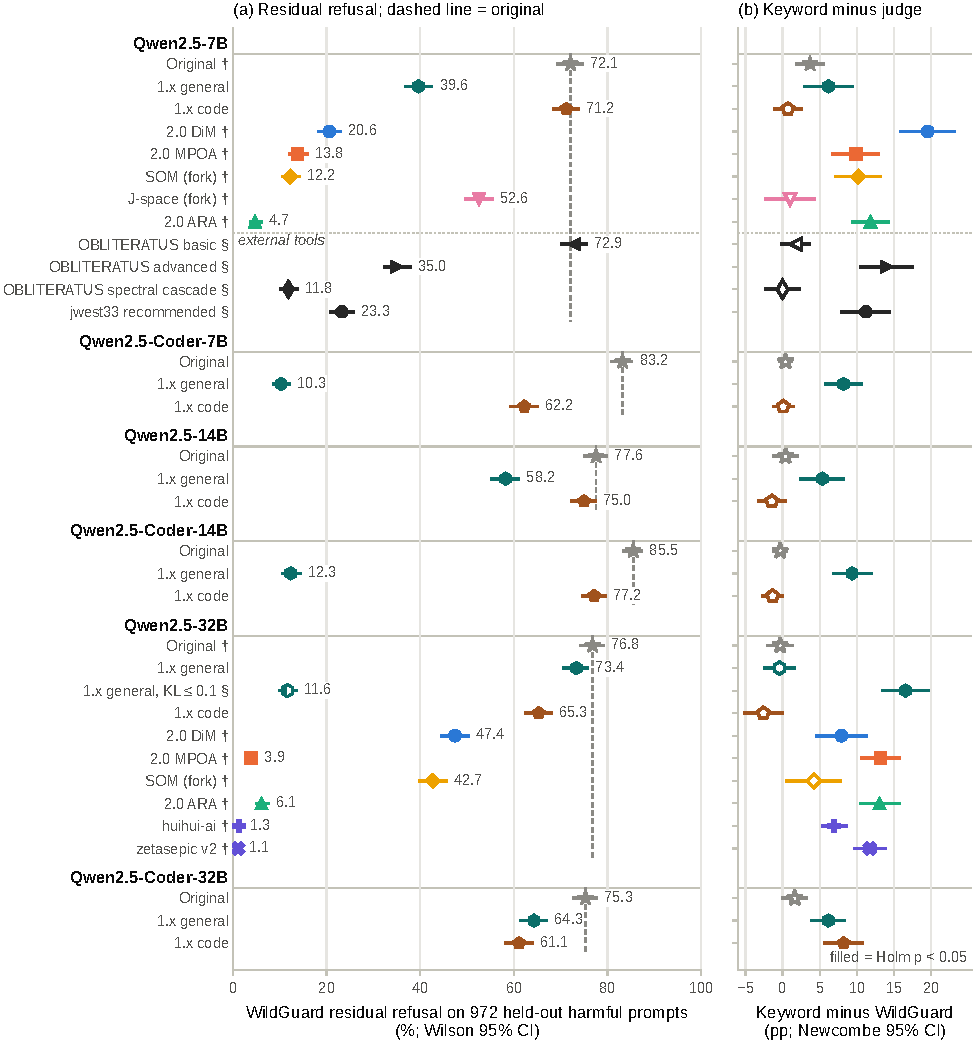
\includegraphics[width=\textwidth]{figures/fig1_residual_refusal.pdf}
\caption{\textbf{Residual refusal by model and condition (held-out, judged; Qwen2.5 models).} (a) Share of the 972
harmful held-out prompts whose response WildGuard labels a refusal, with Wilson 95\% intervals; the dashed line marks
the model's original. (b) Keyword refusal rate minus WildGuard refusal rate on the same responses, with Newcombe 95\%
intervals; filled markers are significant after Holm correction, over the 29 cells of the main design and separately
over the 13 added cells. $\S$ = cell added after the main design (the KL $\le$ 0.1 re-export on Qwen2.5-32B and the
external tools on Qwen2.5-7B, run once at their own settings); the Qwen3.5-4B cells are in
Figure~\ref{fig:tradeoff}c,d and Table~\ref{tab:external}. Heretic~1.x
(teal hexagons, sienna pentagons) was selected at dev KL $\le$ 0.01 (half-filled hexagon: the re-export at dev KL
$\le$ 0.1), Heretic~2.0 and the fork plug-ins at dev KL $\le$ 0.1; ``(fork)'' marks plug-ins of the companion study's project fork, not part of Heretic~2.0; the community
releases are public Qwen2.5-32B abliterations. $\dagger$ = cell first reported in the companion study
\cite{young2026harder}.}
\label{fig:refusal}
\end{figure*}

\subsection{Like-for-Like Version Contrast (H1)}

% src (RESULTS.md "H1 -- Heretic 1.x vs Heretic 2.0 on the same base"; tests_refusal.csv family h1_1x_vs_2.0
%      (n_in_family 18) judges wg/kw/q3g, groups harmful_all/harmful_excl_advbench/benign_all; cells.csv dev_*,
%      tf_divergence, capability_mean_delta_*; supp_stats logic: h1 over-refusal 32B primary wg 2.3 vs 0.6 p=0.773,
%      kw 13.1 vs 12.0 p=1.000, q3g 5.1 vs 2.6 p=0.043; 32B family: wg 0/8, kw 2/8, q3g 3/8)
In the like-for-like contrast on Qwen2.5-32B, 1.x general left 73.4\% of the harmful prompts refused and 2.0 DiM
47.4\%, a paired difference of +25.9~pp [23.0, 28.7]; 259 prompts were refused by the 1.x model only and 7 by the
DiM model only ($p_\mathrm{Holm}<0.001$; Table~\ref{tab:h1}). The difference remained significant under keyword
matching, under Qwen3Guard and without the AdvBench-overlap prompts. Both released trials had kept 89 of 100 dev
refusals, at a dev KL of 0.006 (1.x) and 0.018 (DiM) and a TF divergence of 0.007 and 0.017 nats per token. Neither
model changed capability measurably (mean change +0.19~pp [$-$1.06, +1.45] for 1.x general and $-$0.05~pp
[$-$1.35, +1.25] for DiM). Over-refusal did not differ under WildGuard (2.3\% vs.\ 0.6\%, $p_\mathrm{Holm}=0.77$)
or keyword matching (13.1\% vs.\ 12.0\%, $p_\mathrm{Holm}=1.00$) but was higher for 1.x under Qwen3Guard (5.1\% vs.\
2.6\%, $p_\mathrm{Holm}=0.043$). The difference equals the threshold of two standard deviations of the difference
between two independently optimised cells that the companion study estimated from seed replicates of its
Qwen2.5-7B and Qwen3.5-4B cells (25.9~pp [18.1, 45.4]) \cite{young2026harder}.

% src (tests_refusal.csv h1_1x_vs_2.0, model qwen2.5-7b: general vs dim wg +19.0 [16.1,21.9] 215/30; kw +5.7
%      [2.5,8.8] p=0.0005; q3g +21.2 [18.3,24.0]; excl adv +17.7 [14.7,20.6]; benign wg 1.1 vs 0.3, kw 7.7 vs 8.3,
%      q3g 2.6 vs 1.7, all p_holm=1; cells.csv: 7B 1.x general dev 67 @ 0.0053, tf 0.0089, cap -0.36 [-1.35,0.63];
%      7B dim dev 55 @ 0.0782, tf 0.0194, cap +0.23 [-0.85,1.32])
On Qwen2.5-7B, 1.x general left 39.6\% [36.6, 42.7] of the harmful prompts refused and 2.0 DiM 20.6\% [18.2, 23.2],
a paired difference of +19.0~pp [16.1, 21.9]; 215 prompts were refused by the 1.x model only and 30 by the DiM model
only ($p_\mathrm{Holm}<0.001$). The difference remained significant under keyword matching (+5.7~pp [2.5, 8.8],
$p_\mathrm{Holm}<0.001$), under Qwen3Guard (+21.2~pp [18.3, 24.0]) and without the AdvBench-overlap prompts
(+17.7~pp [14.7, 20.6]). The released 1.x trial had kept 67 of 100 dev refusals at a dev KL of 0.005, the DiM trial
55 at 0.078; their TF divergences were 0.009 and 0.019 nats per token. Neither model changed capability measurably
($-$0.36~pp [$-$1.35, +0.63] and +0.23~pp [$-$0.85, +1.32]), and over-refusal did not differ under any judge
(WildGuard 1.1\% vs.\ 0.3\%, keyword matching 7.7\% vs.\ 8.3\%, Qwen3Guard 2.6\% vs.\ 1.7\%; $p_\mathrm{Holm}=1.00$
each). H1 was therefore supported for the released checkpoints on both base models: on Qwen2.5-32B by a difference
equal to the companion study's seed-noise threshold and on Qwen2.5-7B by a difference below it.
Section~\ref{sec:res-kl} repeats the Qwen2.5-32B contrast with both arms selected by the same rule.

% src (tests_refusal.csv h1_1x_vs_2.0: 32B 8/8 and 7B 10/10 significant under wg, kw, q3g and harmful_excl_advbench
%      with identical signs; benign: 7B wg 5/10 (all 1.x code), kw 2/10 (1.x code vs mpoa, som), q3g 5/10 (all 1.x
%      code); tests_capability.csv original_design: 0 of 115 Holm-significant, min p 0.0166 (7b 1.x code gsm8k
%      +3.2 [0.7,5.8]), next 0.0215 (32b ara humaneval -4.9 [-9.3,-0.9]))
The additional configurations on Qwen2.5-32B all left less residual refusal than both released 1.x variants
(selected at dev KL $\le$ 0.01; \S\ref{sec:res-kl}): 1.x general
exceeded SOM (fork plug-in) by 30.7~pp, ARA by 67.3~pp and MPOA by 69.4~pp [66.4, 72.2], and 1.x code exceeded the
four configurations by 17.9 to 61.4~pp. The discordant prompts ran almost entirely in one direction; for example, 675
prompts were refused by 1.x general and not by MPOA, and none the other way. On Qwen2.5-7B, 1.x general left more
residual refusal than MPOA (+25.8~pp [22.8, 28.8]), SOM (+27.4~pp [24.4, 30.3]) and ARA (+34.9~pp [31.8, 37.9]) and
less than J-space (fork plug-in; $-$13.0~pp [$-$15.6, $-$10.3]; 32 versus 158 discordant prompts); 1.x code, which
had removed no significant refusal, exceeded all five configurations, by 18.6~pp (J-space) to 66.5~pp (ARA). All 18
contrasts were significant ($p_\mathrm{Holm}<0.001$) with the same sign under WildGuard, keyword matching and
Qwen3Guard and without the AdvBench-overlap prompts. Over-refusal differed in none of the Qwen2.5-32B contrasts under
WildGuard, in two under keyword matching and in three under Qwen3Guard (including the primary contrast); on
Qwen2.5-7B it differed only in contrasts of 1.x code (five under WildGuard and Qwen3Guard, two under keyword
matching), whose 5.1\% WildGuard over-refusal exceeded the 0.0--1.1\% of the 2.0 and fork models. No per-benchmark
capability change of any edited model of the main design was significant after Holm correction (115 tests; the
smallest unadjusted $p$ was 0.017, for a GSM8K gain of +3.2~pp [0.7, 5.8] after 1.x code on Qwen2.5-7B, followed by
0.021 for a HumanEval change of $-$4.9~pp [$-$9.3, $-$0.9] after 2.0 ARA on Qwen2.5-32B;
Appendix~\ref{app:capability}).

% KL-matched rows are panel (b) of tables/tab_h1.tex (checked 2026-11-06); no separate tab:h1-kl.
\begin{table*}[tbp]
\centering\small
\caption{H1: Heretic~1.x versus Heretic~2.0 and fork plug-ins on the same base model (WildGuard residual refusal on
the 972 harmful prompts). Primary = like-for-like contrast (1.x general versus 2.0 DiM, the same edit;
Table~\ref{tab:h1setup}); additional = configurations that also change the edit. ``(fork)'' = plug-in of the
companion study's project fork, not part of Heretic~2.0. Differences are paired (Newcombe 95\% CI); 1.x-only /
comp.-only are prompts refused by one model only; $p_\mathrm{Holm}$ from exact McNemar tests; the last column
repeats the test with keyword matching. (a) Released trials, Holm over the 18 1.x-versus-2.0 contrasts
(conservative for the primary contrasts). (b) Added after the main results: trial~\#96 of the archived Qwen2.5-32B
1.x general search, re-exported at the 2.0 selection rule (\S\ref{sec:reexport}), against the same comparators
(KL-matched, Holm over these four contrasts) and against the released trial~\#84 of the same search (cap only, a
single unadjusted test).}
\label{tab:h1}
\setlength{\tabcolsep}{4pt}
\resizebox{\textwidth}{!}{\begin{tabular}{@{}llllrrrrrr@{}}
\toprule
Model & Contrast & 1.x variant & Comparator & 1.x (\%) & Comparator (\%) & 1.x $-$ comparator (pp) [95\% CI] & 1.x-only / comp.-only & $p_\mathrm{Holm}$ & keyword $p_\mathrm{Holm}$ \\
\midrule
\multicolumn{10}{@{}l}{\textit{(a) Pre-stated design: released trials (1.x selected at dev KL $\le$ 0.01, 2.0 and fork at dev KL $\le$ 0.1); Holm over the 18 contrasts}} \\
\addlinespace[1pt]
Qwen2.5-32B & primary & general & 2.0 DiM & 73.4 & 47.4 & +25.9 [+23.0, +28.7] & 259 / 7 & $<$0.001 & $<$0.001 \\
\addlinespace[1pt]
 & additional & general & 2.0 MPOA & 73.4 & 3.9 & +69.4 [+66.4, +72.2] & 675 / 0 & $<$0.001 & $<$0.001 \\
 & additional & general & 2.0 ARA & 73.4 & 6.1 & +67.3 [+64.2, +70.1] & 655 / 1 & $<$0.001 & $<$0.001 \\
 & additional & general & SOM (fork) & 73.4 & 42.7 & +30.7 [+27.7, +33.5] & 300 / 2 & $<$0.001 & $<$0.001 \\
 & additional & code & 2.0 DiM & 65.3 & 47.4 & +17.9 [+15.3, +20.4] & 183 / 9 & $<$0.001 & $<$0.001 \\
 & additional & code & 2.0 MPOA & 65.3 & 3.9 & +61.4 [+58.2, +64.4] & 599 / 2 & $<$0.001 & $<$0.001 \\
 & additional & code & 2.0 ARA & 65.3 & 6.1 & +59.3 [+55.9, +62.4] & 585 / 9 & $<$0.001 & $<$0.001 \\
 & additional & code & SOM (fork) & 65.3 & 42.7 & +22.6 [+19.8, +25.3] & 228 / 8 & $<$0.001 & $<$0.001 \\
\addlinespace[2pt]
Qwen2.5-7B & primary & general & 2.0 DiM & 39.6 & 20.6 & +19.0 [+16.1, +21.9] & 215 / 30 & $<$0.001 & $<$0.001 \\
\addlinespace[1pt]
 & additional & general & 2.0 MPOA & 39.6 & 13.8 & +25.8 [+22.8, +28.8] & 269 / 18 & $<$0.001 & $<$0.001 \\
 & additional & general & 2.0 ARA & 39.6 & 4.7 & +34.9 [+31.8, +37.9] & 344 / 5 & $<$0.001 & $<$0.001 \\
 & additional & general & SOM (fork) & 39.6 & 12.2 & +27.4 [+24.4, +30.3] & 278 / 12 & $<$0.001 & $<$0.001 \\
 & additional & general & J-space (fork) & 39.6 & 52.6 & $-$13.0 [$-$15.6, $-$10.3] & 32 / 158 & $<$0.001 & $<$0.001 \\
 & additional & code & 2.0 DiM & 71.2 & 20.6 & +50.6 [+47.3, +53.7] & 495 / 3 & $<$0.001 & $<$0.001 \\
 & additional & code & 2.0 MPOA & 71.2 & 13.8 & +57.4 [+54.1, +60.4] & 561 / 3 & $<$0.001 & $<$0.001 \\
 & additional & code & 2.0 ARA & 71.2 & 4.7 & +66.5 [+63.3, +69.3] & 647 / 1 & $<$0.001 & $<$0.001 \\
 & additional & code & SOM (fork) & 71.2 & 12.2 & +59.0 [+55.7, +61.9] & 574 / 1 & $<$0.001 & $<$0.001 \\
 & additional & code & J-space (fork) & 71.2 & 52.6 & +18.6 [+16.0, +21.2] & 189 / 8 & $<$0.001 & $<$0.001 \\
\midrule
\multicolumn{10}{@{}l}{\textit{(b) Added: the original 1.x general study re-exported at the 2.0 selection rule (dev KL $\le$ 0.1; trial \#96); separate Holm families}} \\
\addlinespace[1pt]
Qwen2.5-32B & KL-matched & general, \#96 & 2.0 DiM & 11.6 & 47.4 & $-$35.8 [$-$38.9, $-$32.7] & 5 / 353 & $<$0.001 & $<$0.001 \\
 & KL-matched & general, \#96 & 2.0 MPOA & 11.6 & 3.9 & +7.7 [+5.9, +9.7] & 83 / 8 & $<$0.001 & $<$0.001 \\
 & KL-matched & general, \#96 & 2.0 ARA & 11.6 & 6.1 & +5.6 [+3.6, +7.6] & 77 / 23 & $<$0.001 & $<$0.001 \\
 & KL-matched & general, \#96 & SOM (fork) & 11.6 & 42.7 & $-$31.1 [$-$34.0, $-$28.1] & 6 / 308 & $<$0.001 & $<$0.001 \\
\addlinespace[1pt]
 & cap only & general, \#96 & general, \#84 & 11.6 & 73.4 & $-$61.7 [$-$64.7, $-$58.5] & 2 / 602 & $<$0.001 & $<$0.001 \\
\bottomrule
\multicolumn{10}{@{}l}{\footnotesize Panel (b): KL-matched rows, Holm over 4 contrasts (family \texttt{h1\_kl\_matched}); cap-only row, a single test (family \texttt{kl\_cap\_1x}).} \\
\multicolumn{10}{@{}l}{\footnotesize \#84: the released 1.x general model of panel (a) (dev KL 0.006); \#96: fewest dev refusals at dev KL $\le$ 0.1 (KL 0.064); same study, journal and heretic-llm 1.4.0.} \\
\multicolumn{10}{@{}l}{\footnotesize KL-matched: both sides selected by the same rule (fewest dev refusals at dev KL $\le$ 0.1); realised dev KL still differs (Table~\ref{tab:devkl}). One optimisation run per condition.} \\
\end{tabular}
}
\end{table*}

\subsection{Like-for-Like Contrast at the Same Selection Rule}
\label{sec:res-kl}

% src (RESULTS.md "1.x general re-exported at KL <= 0.1 (trial #96) vs Heretic 2.0" and "1.x general at KL <= 0.1
%      vs the original 1.x export at KL <= 0.01"; tests_refusal.csv families h1_kl_matched (n_in_family 4) and
%      kl_cap_1x (1): wg/kw/q3g/excl-adv all same sign and p_holm < 0.001; kw: dim -27.2, som -18.7, mpoa +11.1,
%      ara +9.1; seed-noise threshold: paper 33 seednoise_summary.md)
The 1.x general model selected by the 2.0 rule from the archived Qwen2.5-32B search (trial~\#96;
\S\ref{sec:reexport}) left 11.6\% [9.8, 13.8] of the harmful prompts refused, against 73.4\% for the released
export of the same search (dev KL $\le$ 0.01) and 76.8\% for the original (Table~\ref{tab:h1}). The paired
difference between the two exports of the same search was $-$61.7~pp [$-$64.7, $-$58.5]: 602 prompts were refused
only by the KL $\le$ 0.01 export and 2 only by the KL $\le$ 0.1 export ($p<0.001$). Against the configurations on
the same base model, the KL $\le$ 0.1 export left 35.8~pp [32.7, 38.9] less residual refusal than 2.0 DiM (5 versus
353 discordant prompts) and 31.1~pp [28.1, 34.0] less than SOM (fork plug-in), and 7.7~pp [5.9, 9.7] more than MPOA
(83 versus 8) and 5.6~pp [3.6, 7.6] more than ARA (77 versus 23); all four $p_\mathrm{Holm}<0.001$. Each contrast
had the same sign and remained significant under keyword matching, under Qwen3Guard and without the AdvBench-overlap
prompts. With both arms of the like-for-like contrast selected by the same rule, the order therefore reversed: the
1.x general model left less residual refusal than 2.0 DiM, by a difference larger than the companion study's
seed-noise threshold (25.9~pp [18.1, 45.4]). This comparison rests on one search per arm (one seed each) on one base
model, and the two arms still differed in trial budget, search seed, optimisation system prompt and marker list
(Table~\ref{tab:h1setup}).

% src (cells.csv qwen2.5-32b__heretic1x-general-kl0.1: dev 50 @ 0.0642, reeval 51 @ 0.0637, tf 0.0323,
%      capability +0.02 [-1.27,1.31], overrefusal_wg 0.0, hb_harm 0.746, degenerate 1/972, kw 28.2; tf of
%      qwen2.5-32b__{heretic1x-general 0.0066, dim 0.0165, som 0.0202, mpoa 0.0416, ara 0.0773}; hb_harm 1.x 0.221,
%      dim 0.403; tests_capability.csv added: none Holm-significant; kl_cap_1x benign wg -2.3 [-4.4,-0.7] p=0.0078;
%      kw_vs_judge_added: +16.6 [13.4,19.7])
The KL $\le$ 0.1 export moved the model further than the released 1.x export, DiM and SOM but less than MPOA and
ARA: its TF divergence was 0.032 nats per token, against 0.007 for the KL $\le$ 0.01 export, 0.017 for DiM, 0.020 for SOM,
0.042 for MPOA and 0.077 for ARA. Its mean capability change was +0.02~pp [$-$1.27, +1.31], and no benchmark change
was significant. WildGuard over-refusal on the benign prompts was 0.0\%, against 2.3\% for the KL $\le$ 0.01 export
($-$2.3~pp [$-$4.4, $-$0.7], $p=0.008$); harmful compliance by the HarmBench classifier was 74.6\%, against 22.1\%
for the KL $\le$ 0.01 export and 40.3\% for DiM; and 1 of its 972 harmful responses was degenerate. Keyword matching
counted 28.2\% of its harmful responses as refusals, 16.6~pp [13.4, 19.7] more than WildGuard. No KL-matched cell
exists for the 1.x code variant or for Qwen2.5-7B (\S\ref{sec:reexport}).

\subsection{Source of the Refusal Direction (H2)}

% src (RESULTS.md "H2 -- 1.x general vs 1.x code, by item group"; tests_refusal.csv h2_general_vs_code (n_in_family
%      6); cells.csv wg_code_rate / wg_noncode_rate of the six originals (code 13.5-34.0, non-code 87.3-98.8);
%      tf_divergence of the 12 1.x cells)
The originals refused only 13.5\% (Qwen2.5-7B) to 34.0\% (Qwen2.5-Coder-14B) of the code-as-weapon prompts,
against 87.3\% to 98.8\% of the other harmful prompts (Figure~\ref{fig:general-code}). H2 predicted a crossover: the
code variant lower than the general variant on code-as-weapon prompts and higher on non-code prompts. No model showed
this crossover (Table~\ref{tab:h2}). On Qwen2.5-7B, Qwen2.5-Coder-7B, Qwen2.5-14B and Qwen2.5-Coder-14B the code
variant left more residual refusal on both subsets (code-as-weapon 12.0\% vs.\ 2.0\%, 8.0\% vs.\ 0.5\%, 14.5\% vs.\
5.5\% and 16.0\% vs.\ 0.0\%; non-code 86.5\% vs.\ 49.4\%, 76.3\% vs.\ 12.8\%, 90.7\% vs.\ 71.9\% and 93.0\% vs.\
15.5\%). Without the 41 prompts drawn from the code variant's source corpora, the code-as-weapon differences on
Qwen2.5-7B ($-$6.3~pp [$-$11.3, $-$2.5], $p_\mathrm{Holm}=0.010$) and on both 14B models remained significant and
that on Qwen2.5-Coder-7B did not ($-$3.8~pp [$-$8.0, $-$0.7], $p_\mathrm{Holm}=0.094$). On Qwen2.5-32B the code
variant left less on both subsets (code-as-weapon 6.5\% vs.\ 12.0\%; non-code 80.6\% vs.\ 89.2\%), and without the
41 prompts the code-as-weapon difference was +3.1~pp [$-$0.5, +7.4] ($p_\mathrm{Holm}=0.250$). On
Qwen2.5-Coder-32B the code variant left less on non-code prompts (74.6\% vs.\ 78.6\%) and the same on code-as-weapon
prompts (9.0\% each). In all six models, the variant that left less residual refusal on one subset left less or equal
residual refusal on the other. The code variant's released models diverged less from their originals than the
general variant's on Qwen2.5-Coder-7B and both 14B models (TF divergence 0.008, 0.006 and 0.007 vs.\ 0.017, 0.018
and 0.020 nats per token), more on Qwen2.5-7B (0.075 vs.\ 0.009) and Qwen2.5-32B (0.017 vs.\ 0.007) and equally on
Qwen2.5-Coder-32B (0.004 each). H2 was not supported.

\begin{figure}[tbp]
\centering
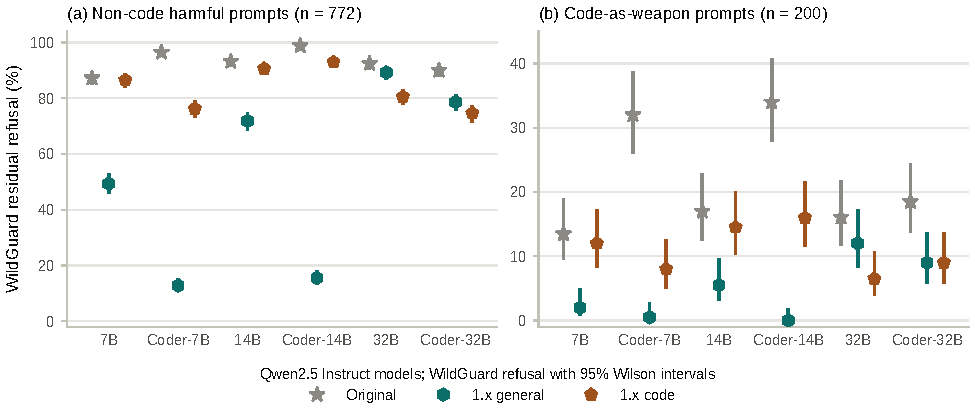
\includegraphics[width=\textwidth]{figures/fig3_general_vs_code.pdf}
\caption{\textbf{Heretic~1.x general versus code variant (H2).} WildGuard residual refusal with Wilson 95\%
intervals for the original (grey star), the 1.x general variant (direction from \texttt{harmful\_behaviors} versus
\texttt{harmless\_alpaca}) and the 1.x code variant (direction from malicious- versus benign-code prompts) on
(a) the 772 non-code harmful prompts and (b) the 200 code-as-weapon prompts; the panels use different vertical
scales. H2 predicted the code variant to be lower in (b) and higher in (a). No model showed this crossover: the code
variant was higher in both panels on the two 7B and the two 14B models, lower in both on Qwen2.5-32B (in (b) not
significantly once the 41 prompts from its source corpora are excluded) and lower in (a) and equal in (b) on
Qwen2.5-Coder-32B.}
\label{fig:general-code}
\end{figure}

\begin{table}[tbp]
\centering\small
\caption{H2: Heretic~1.x general versus code variant by prompt subset (WildGuard residual refusal; paired
Newcombe 95\% CI; exact McNemar, Holm over the six models within each subset). A negative difference means that
the general variant left less residual refusal.}
\label{tab:h2}
\setlength{\tabcolsep}{3pt}
\resizebox{\textwidth}{!}{\begin{tabular}{@{}llrrrr@{}}
\toprule
Model & Prompt subset ($n$) & General (\%) & Code (\%) & General $-$ code (pp) [95\% CI]; $<0$: general lower & $p_\mathrm{Holm}$ \\
\midrule
Qwen2.5-7B & Non-code harmful (772) & 49.4 & 86.5 & $-$37.2 [$-$40.6, $-$33.7] & $<$0.001 \\
 & Code-as-weapon (200) & 2.0 & 12.0 & $-$10.0 [$-$15.0, $-$6.0] & $<$0.001 \\
 & Code-as-weapon, excl.\ RMCBench/MalwareBench (159) & 1.9 & 8.2 & $-$6.3 [$-$11.3, $-$2.5] & 0.010 \\
\addlinespace[2pt]
Qwen2.5-Coder-7B & Non-code harmful (772) & 12.8 & 76.3 & $-$63.5 [$-$66.8, $-$59.8] & $<$0.001 \\
 & Code-as-weapon (200) & 0.5 & 8.0 & $-$7.5 [$-$12.1, $-$3.9] & $<$0.001 \\
 & Code-as-weapon, excl.\ RMCBench/MalwareBench (159) & 0.0 & 3.8 & $-$3.8 [$-$8.0, $-$0.7] & 0.094 \\
\addlinespace[2pt]
Qwen2.5-14B & Non-code harmful (772) & 71.9 & 90.7 & $-$18.8 [$-$21.7, $-$16.0] & $<$0.001 \\
 & Code-as-weapon (200) & 5.5 & 14.5 & $-$9.0 [$-$13.7, $-$5.1] & $<$0.001 \\
 & Code-as-weapon, excl.\ RMCBench/MalwareBench (159) & 3.8 & 8.8 & $-$5.0 [$-$9.6, $-$1.4] & 0.031 \\
\addlinespace[2pt]
Qwen2.5-Coder-14B & Non-code harmful (772) & 15.5 & 93.0 & $-$77.5 [$-$80.2, $-$74.3] & $<$0.001 \\
 & Code-as-weapon (200) & 0.0 & 16.0 & $-$16.0 [$-$21.7, $-$11.2] & $<$0.001 \\
 & Code-as-weapon, excl.\ RMCBench/MalwareBench (159) & 0.0 & 9.4 & $-$9.4 [$-$15.0, $-$5.1] & $<$0.001 \\
\addlinespace[2pt]
Qwen2.5-32B & Non-code harmful (772) & 89.2 & 80.6 & +8.7 [+6.4, +11.1] & $<$0.001 \\
 & Code-as-weapon (200) & 12.0 & 6.5 & +5.5 [+1.9, +9.6] & 0.007 \\
 & Code-as-weapon, excl.\ RMCBench/MalwareBench (159) & 7.5 & 4.4 & +3.1 [$-$0.5, +7.4] & 0.250 \\
\addlinespace[2pt]
Qwen2.5-Coder-32B & Non-code harmful (772) & 78.6 & 74.6 & +4.0 [+1.8, +6.2] & $<$0.001 \\
 & Code-as-weapon (200) & 9.0 & 9.0 & 0.0 [$-$3.3, +3.3] & 1.000 \\
 & Code-as-weapon, excl.\ RMCBench/MalwareBench (159) & 5.0 & 5.7 & $-$0.6 [$-$3.9, +2.5] & 1.000 \\
\bottomrule
\end{tabular}
}
\end{table}

\subsection{Keyword Counts versus the Judge (H3)}

% src (RESULTS.md "H3 -- keyword minus WildGuard"; tests_refusal.csv kw_vs_judge (n_in_family 29) judges
%      kw_minus_wg / kw256_minus_wg / kw_minus_q3g; correlations.csv kw_minus_wg_pp vs wg_reduction_pp +0.77
%      [0.53, 0.87] n=23; supp_stats logic on the 29 main-design cells: kw-wg edited 15/23 pos, 0 neg; new 1.x 6/12,
%      -2.6..+9.4; companion 9/11, +1.0..+19.5; kw-q3g 15/23 pos, 0 neg; kw256 12/23 pos, 0 neg, min -4.0 (32B 1.x
%      code, p_holm 0.054); shrink median 2.37 (0.3-5.6); kw-only 2,910, capped 44.6%; all edited harmful 37.7%;
%      WG-not-refusal 57.2%; rank_flips.csv (76 pairs))
Keyword matching and WildGuard agreed closely on the six originals (keyword minus WildGuard $-$0.3 to +3.7~pp,
significant only for Qwen2.5-7B, +3.7~pp [1.8, 5.6]) but not after editing (Figure~\ref{fig:refusal}b). Keyword
matching counted significantly more refusals than WildGuard in 15 of the 23 edited models and significantly fewer in
none; the gap ranged from $-$2.6~pp (1.x code on Qwen2.5-32B) to +19.5~pp (2.0 DiM on Qwen2.5-7B) and was larger for
models from which more refusal had been removed (Spearman $\rho=+0.77$ [0.53, 0.87]). Among the twelve new 1.x
cells the gap was significant in six and ranged from $-$2.6 to +9.4~pp (1.x general on Qwen2.5-Coder-14B); among the
eleven edited companion-study cells it was significant in nine and ranged from +1.0 to +19.5~pp. Against Qwen3Guard
as the reference, keyword matching counted significantly more refusals in the same number of edited models (15 of
23) and fewer in none. With keyword matching restricted to the first 256 tokens, the gaps shrank by a median of
2.4~pp (range 0.3 to 5.6~pp), for example from +19.5 to +17.2~pp for 2.0 DiM on Qwen2.5-7B and from +13.2 to
+8.4~pp for 2.0 MPOA on Qwen2.5-32B; keyword matching then counted significantly more refusals than WildGuard in 12
of 23 edited models and significantly fewer in none (lowest gap $-$4.0~pp, 1.x code on Qwen2.5-32B,
$p_\mathrm{Holm}=0.054$). Of the 2{,}910 harmful responses of edited models that keyword matching but not WildGuard
counted as refusals, 44.6\% had reached the 512-token limit, against 37.7\% of all harmful responses of edited
models and 57.2\% of those that WildGuard did not label as refusals.

Of 76 within-model pairs, one changed sign between keyword matching and WildGuard (huihui-ai versus zetasepic v2:
+0.2~pp under WildGuard, not significant; $-$4.6~pp under keyword matching, $p_\mathrm{Holm}<0.001$), two differences
were significant under WildGuard only (MPOA versus ARA on Qwen2.5-32B, $-$2.2~pp, $p_\mathrm{Holm}=0.015$; 1.x
general versus code on Qwen2.5-Coder-32B, +3.2~pp, $p_\mathrm{Holm}=0.004$), and two under keyword matching only
(huihui-ai versus zetasepic v2, and the Qwen2.5-7B original versus its 1.x code variant: +0.9~pp under WildGuard,
not significant; +3.9~pp under keyword matching, $p_\mathrm{Holm}<0.001$). Every 1.x-versus-2.0 decision (18
contrasts) and every KL-matched decision (4) was the same under both measures, but keyword matching reduced the
primary contrast from +19.0 to +5.7~pp on Qwen2.5-7B and from +25.9 to +17.6~pp on Qwen2.5-32B. H3 was partially
supported: the gap depended on the tool, but within the main design it rarely changed the order of tools. Among the
contrasts of the external tools with Heretic it changed more decisions, including one significant reversal
(\S\ref{sec:res-external}).

\subsection{External Tools}
\label{sec:res-external}

% src (RESULTS.md "Residual refusal and secondary outcomes per cell", "Added cells vs their original", "External
%      tools vs Heretic on the same base", "jwest33 on Qwen3.5-4B: as released vs with the CLI hybrid-detection
%      fix", "Added cells: keyword minus WildGuard", "Not supported", "Anomalies and checks" (degenerate counts);
%      tests_refusal.csv families vs_base_added (12), external_vs_heretic (38), external_sensitivity (1),
%      kw_vs_judge_added (13); tests_capability.csv family added (60 tests); cells.csv ext_self_refusal_rate,
%      degenerate_rate/_lo/_hi, capped_rate, tf_divergence, overrefusal_wg_rate, hb_harm_rate)
% tables/tab_external.tex is a bare tabular (checked 2026-11-06), so it is wrapped here; label tab:external.
\begin{table*}[tbp]
\centering\small
\caption{External tools at their documented default or recommended settings (one run each, seed~1, no search or
selection by the author), with Heretic context rows from the same base model (held-out harmful prompts, WildGuard;
Wilson 95\% CI). Capability $\Delta$: change of the mean of the five benchmarks (paired 95\% CI). TF div.:
teacher-forced divergence from the original on the 350 benign prompts. The tools' own checks use their own prompts,
markers and generation lengths and are not comparable with the held-out measures (\S\ref{sec:external}).}
\label{tab:external}
\setlength{\tabcolsep}{3.5pt}
\resizebox{\textwidth}{!}{\begin{tabular}{@{}lrrrrrrrrr@{}}
\toprule
Condition & \multicolumn{2}{c}{WildGuard refusal,} & Keyword & HarmBench & Over-refusal & Capability $\Delta$ (pp) & TF div. & Degenerate & Tool's own \\
 & \multicolumn{2}{c}{harmful (\%) [95\% CI]} & (\%) & harmful (\%) & benign (\%) & [95\% CI] & (nats/tok.) & (of 972)$^{e}$ & check (\%)$^{f}$ \\
\midrule
\multicolumn{10}{@{}l}{\textbf{Qwen2.5-7B}} \\
\quad \textit{Original} & 72.1 & [69.2, 74.8] & 75.8 & 23.3 & 4.3 & -- & -- & 2 & -- \\
\quad \textit{Heretic 1.x general} & 39.6 & [36.6, 42.7] & 45.8 & 45.6 & 1.1 & $-$0.36 [$-$1.35, +0.63] & 0.009 & 2 & 67.0 (100) \\
\quad \textit{Heretic 2.0 ARA}$^{a}$ & 4.7 & [3.6, 6.3] & 16.6 & 79.0 & 0.0 & +0.48 [$-$0.76, +1.72] & 0.048 & 5 & 8.0 (100) \\
\quad OBLITERATUS basic & 72.9 & [70.1, 75.6] & 74.7 & 22.8 & 5.7 & $-$0.79 [$-$1.91, +0.33] & 0.058 & 2 & 83.3 (30) \\
\quad OBLITERATUS advanced & 35.0 & [32.1, 38.1] & 49.0 & 51.4 & 0.0 & $-$0.97 [$-$2.30, +0.36] & 0.158 & 30 & 40.0 (30) \\
\quad OBLITERATUS spectral cascade & 11.8 & [9.9, 14.0] & 11.8 & 72.8 & 0.6 & $-$5.18 [$-$6.90, $-$3.47] & 0.471 & 56 & 3.3 (30) \\
\quad jwest33 recommended$^{b}$ & 23.3 & [20.7, 26.0] & 34.5 & 62.6 & 0.0 & $-$0.15 [$-$1.38, +1.08] & 0.029 & 6 & n.r. \\
\addlinespace[3pt]
\multicolumn{10}{@{}l}{\textbf{Qwen3.5-4B}} \\
\quad \textit{Original} & 88.5 & [86.3, 90.3] & 89.2 & 9.5 & 9.7 & -- & -- & 0 & -- \\
\quad \textit{Heretic 2.0 MPOA}$^{a}$ & 18.0 & [15.7, 20.5] & 23.6 & 55.9 & 0.0 & $-$0.52 [$-$1.51, +0.47] & 0.031 & 3 & 6.0 (100) \\
\quad OBLITERATUS, any preset & \multicolumn{9}{l}{not supported: v0.1.4 does not support the Qwen3.5 hybrid-attention architecture; no model produced} \\
\quad jwest33, as released$^{c}$ & 1.0 & [0.6, 1.9] & 9.9 & 81.3 & 0.0 & $-$0.37 [$-$1.73, +0.99] & 0.132 & 0 & n.r. \\
\quad jwest33 + hybrid fix$^{d}$ & 35.8 & [32.8, 38.9] & 39.4 & 42.9 & 0.0 & $-$0.22 [$-$1.52, +1.08] & 0.035 & 0 & n.r. \\
\bottomrule
\multicolumn{10}{@{}l}{\footnotesize Italic: context rows (original, Heretic). External tools: run once by the author with their documented default or recommended settings (OBLITERATUS v0.1.4,} \\
\multicolumn{10}{@{}l}{\footnotesize \phantom{Italic: }commit 461ff086; jwest33/abliterator, commit 6ca3356e; seed 1); same evaluation harness as all other cells.} \\
\multicolumn{10}{@{}l}{\footnotesize $^{a}$ Best Heretic 2.0: lowest WildGuard refusal among DiM, MPOA and ARA (fork plug-ins excluded); companion study \cite{young2026harder}. No 1.x cell for Qwen3.5-4B.} \\
\multicolumn{10}{@{}l}{\footnotesize $^{b}$ Run with the patch of $^{d}$; Qwen2.5-7B is not hybrid (\texttt{is\_hybrid} = false), so the patch is a no-op and the model is effectively as released.} \\
\multicolumn{10}{@{}l}{\footnotesize $^{c}$ Primary. As released: the CLI path omits the hybrid-architecture detection, so the default \texttt{-{}-hybrid-strategy auto} has no effect.} \\
\multicolumn{10}{@{}l}{\footnotesize $^{d}$ Sensitivity analysis: runtime patch that sets the hybrid-architecture information before direction extraction, as the library path does.} \\
\multicolumn{10}{@{}l}{\footnotesize $^{e}$ Harmful responses flagged degenerate by the harness (repetition or character run).} \\
\multicolumn{10}{@{}l}{\footnotesize $^{f}$ Refusal rate (\%) the tool reports for its own check (number of prompts). OBLITERATUS: post-edit quality check on 30 of its 842} \\
\multicolumn{10}{@{}l}{\footnotesize \phantom{$^{f}$} built-in harmful prompts. Heretic: dev keyword refusals of the released trial (100 prompts). n.r.: not reported by the tool.} \\
\end{tabular}
}
\end{table*}

Table~\ref{tab:external} summarises the external-tool cells. On Qwen2.5-7B (original 72.1\%), OBLITERATUS
\texttt{basic} did not reduce refusal: it left 72.9\% [70.1, 75.6] of the harmful prompts refused (+0.8~pp [$-$0.6, +2.3] against the original, $p_\mathrm{Holm}=0.33$), with no significant
change under keyword matching or Qwen3Guard either. The tool's own check agreed: it reported a refusal rate of 83\% on
its 30-prompt verification sample. \texttt{advanced} left 35.0\% [32.1, 38.1] ($-$37.2~pp [$-$40.3, $-$33.9]; own
check 40\%) and \texttt{spectral\_cascade} 11.8\% [9.9, 14.0] ($-$60.3~pp [$-$63.3, $-$57.0]; own check 3\%), both
$p_\mathrm{Holm}<0.001$. The tool's own checks therefore ranked the three presets in the same order as the held-out
judge. jwest33's abliterator, in effect as released, left 23.3\% [20.7, 26.0] on Qwen2.5-7B ($-$48.9~pp [$-$51.9,
$-$45.6], $p_\mathrm{Holm}<0.001$); its batch run reports no refusal rate of its own, so no agreement check was
possible. OBLITERATUS produced no model for Qwen3.5-4B (not supported).

% src (cells.csv tf_divergence: basic 0.058, advanced 0.158, spectral 0.471, jwest33-7b 0.029; 7B Heretic cells
%      0.009-0.075 (1.x code 0.0749; 2.0/fork max ara 0.0484); capability_mean_delta: basic -0.79 [-1.91,0.33],
%      advanced -0.97 [-2.30,0.36], spectral -5.18 [-6.90,-3.47], jwest33 -0.15 [-1.38,1.08];
%      tests_capability.csv added: spectral mmlu_pro -7.0 [-9.9,-4.0] p_holm 0.0003; humaneval -9.1 [-15.0,-3.5]
%      p 0.0026 p_holm 0.15; degenerate 30/972 (3.1% [2.2,4.4]), 56/972 (5.8% [4.5,7.4]), base 2, Heretic 7B <= 5,
%      jwest33 6; hb_harm basic 22.8, advanced 51.4, spectral 72.8, jwest33 62.6, base 23.3; overrefusal_wg basic 5.7,
%      advanced 0.0, spectral 0.6, jwest33 0.0, base 4.3 (basic vs base p_holm 0.227))
\texttt{advanced} and \texttt{spectral\_cascade} moved the model further than any Heretic model on Qwen2.5-7B,
\texttt{basic} further than all but 1.x code, and jwest33 further than all but ARA and 1.x code: their TF
divergences were 0.058 (\texttt{basic}), 0.158 (\texttt{advanced}) and 0.471 nats per token
(\texttt{spectral\_cascade}) and 0.029 for jwest33, against 0.009 to 0.048 for the 2.0, fork and 1.x general models
and 0.075 for 1.x code. \texttt{spectral\_cascade} was the only edited model in the study whose mean capability change
excluded zero ($-$5.18~pp [$-$6.90, $-$3.47]); its MMLU-Pro change ($-$7.0~pp [$-$9.9, $-$4.0]) was significant after
Holm correction over the 60 capability tests of the added cells, and its HumanEval change ($-$9.1~pp [$-$15.0,
$-$3.5]) was not. The mean changes of \texttt{basic} ($-$0.79~pp [$-$1.91, +0.33]), \texttt{advanced} ($-$0.97~pp
[$-$2.30, +0.36]) and jwest33 ($-$0.15~pp [$-$1.38, +1.08]) included zero. Degenerate responses were frequent only
for two OBLITERATUS presets: 56 of the 972 harmful responses of \texttt{spectral\_cascade} (5.8\% [4.5, 7.4]) and 30
of \texttt{advanced} (3.1\% [2.2, 4.4]), against 2 for the original, at most 5 for any Heretic model on Qwen2.5-7B and
6 for jwest33. Harmful compliance by the HarmBench classifier was 22.8\% for \texttt{basic} (original 23.3\%), 51.4\%
for \texttt{advanced}, 72.8\% for \texttt{spectral\_cascade} and 62.6\% for jwest33. WildGuard over-refusal fell to
0.0--0.6\% for the three external-tool models that removed refusal and was 5.7\% for \texttt{basic} (original 4.3\%,
$p_\mathrm{Holm}=0.23$).

% src (tests_refusal.csv external_vs_heretic, judge wg, harmful_all (n_in_family 38))
Against the Heretic cells on Qwen2.5-7B (WildGuard), \texttt{spectral\_cascade} left 8.7~pp [6.2, 11.3] less residual
refusal than 2.0 DiM, did not differ significantly from MPOA ($-$2.0~pp [$-$4.3, +0.4], $p_\mathrm{Holm}=0.23$) or
SOM ($-$0.4~pp, $p_\mathrm{Holm}=0.79$) and left 7.1~pp [5.2, 9.1] more than ARA. \texttt{advanced} left more than
DiM, MPOA, SOM and ARA (by 14.4 to 30.3~pp) and less than J-space ($-$17.6~pp), 1.x code ($-$36.3~pp) and 1.x
general ($-$4.6~pp [$-$7.7, $-$1.6], $p_\mathrm{Holm}=0.017$; without the AdvBench-overlap prompts $-$3.1~pp,
$p_\mathrm{Holm}=0.15$).
\texttt{basic} left more than every Heretic model except 1.x code (+1.7~pp, $p_\mathrm{Holm}=0.13$). jwest33 did not
differ significantly from DiM (+2.7~pp [0.3, 5.1], $p_\mathrm{Holm}=0.13$), left more than MPOA (+9.5~pp), SOM
(+11.0~pp) and ARA (+18.5~pp) and less than J-space ($-$29.3~pp), 1.x general ($-$16.4~pp) and 1.x code
($-$47.9~pp); all of these $p_\mathrm{Holm}<0.001$.

% src (RESULTS.md rows qwen3.5-4b__*; tests_refusal.csv vs_base_added, external_vs_heretic (qwen3.5-4b),
%      external_sensitivity: -34.8 [-37.8,-31.8] 0/338; cells.csv capped_rate asreleased 0.878, hybridfix 0.642,
%      base 0.291; tf asreleased 0.132, hybridfix 0.035, 4B 2.0/fork 0.010-0.093; capability asreleased -0.37
%      [-1.73,0.99], hybridfix -0.22 [-1.52,1.08]; hb_harm 81.3 / 42.9; degenerate 0 / 0; PROVENANCE hybrid_detection)
On Qwen3.5-4B (original 88.5\%), jwest33 as released left 1.0\% [0.6, 1.9] of the harmful prompts refused
($-$87.4~pp [$-$89.4, $-$85.1]; 850 prompts refused only by the original, none only by the edited model), less than
each of the five companion-study models on that base (DiM 54.6\%, MPOA 18.0\%, SOM 21.9\%, J-space 73.8\%, ARA
18.9\%; differences $-$17.0 to $-$72.7~pp, all $p_\mathrm{Holm}<0.001$). Its TF divergence was 0.132 nats per token
(companion models 0.010 to 0.093), its mean capability change $-$0.37~pp [$-$1.73, +0.99], its HarmBench compliance
81.3\%, and none of its harmful responses was degenerate, but 87.8\% of its harmful responses reached the 512-token limit,
against 29.1\% for the original. In the sensitivity run with the hybrid-architecture detection restored, the tool left
35.8\% [32.8, 38.9] refused, 34.8~pp [31.8, 37.8] more than as released (338 versus 0 discordant prompts,
$p<0.001$), at a TF divergence of 0.035 and a mean capability change of $-$0.22~pp [$-$1.52, +1.08]. The sensitivity
cell left less residual refusal than DiM ($-$18.8~pp) and J-space ($-$38.0~pp) and more than MPOA (+17.8~pp), SOM
(+13.9~pp) and ARA (+16.9~pp; all $p_\mathrm{Holm}<0.001$). All Qwen3.5-4B edits reduced WildGuard over-refusal from
9.7\% to at most 1.4\%.

% src (tests_refusal.csv kw_vs_judge_added (13) and external_vs_heretic judge kw vs wg (harmful_all): both-sig
%      opposite 1 (spectral vs ara), wg-only 1 (advanced vs 1.x general), kw-only 4 (spectral vs mpoa, som;
%      jwest33 vs dim; basic vs 1.x code))
The keyword--judge gap of the added cells ranged from $-$21.1~pp (J-space on Qwen3.5-4B, where keyword matching
counted fewer refusals than WildGuard) to +16.6~pp (the KL $\le$ 0.1 re-export). Among the external tools it was
+14.0~pp [10.3, 17.7] for \texttt{advanced}, +11.2~pp [7.9, 14.5] for jwest33 on Qwen2.5-7B and +8.8~pp [6.9, 10.9]
as released on Qwen3.5-4B, but zero for \texttt{spectral\_cascade} (+0.0~pp [$-$2.4, +2.4]) and not significant for
\texttt{basic}. Keyword matching changed 6 of the 38 external-versus-Heretic decisions: it reversed one
significant difference (\texttt{spectral\_cascade} versus ARA: +7.1~pp under WildGuard, $-$4.7~pp under keyword matching, both $p_\mathrm{Holm}<0.01$), removed one (\texttt{advanced}
versus 1.x general) and made four differences significant that WildGuard did not (\texttt{spectral\_cascade} versus
MPOA and SOM, $-$11.8 and $-$10.6~pp; jwest33 versus DiM, $-$5.7~pp; \texttt{basic} versus 1.x code, +2.8~pp).

\subsection{Refusal, Distribution Shift and Capability (Exploratory)}

% src (correlations.csv (23 main-design edited cells): wg_rate~tf -0.75 [-0.93,-0.38]; wg_rate~dev_kl -0.68
%      [-0.83,-0.42] n=21; wg_rate~capability +0.50 [+0.08,+0.79] p=0.016; supp_stats logic (exact permutation):
%      32B n=8 rho -0.93 p=0.0022; 7B n=7 rho -0.18 p=0.71; tf band 0.016-0.021: 11.4 (32B 1.x code, paired) to
%      73.1 (C14B 1.x general); tests_refusal.csv within_model_pairs (76): 32B dim vs 1.x code, mpoa vs ara
%      p_holm 0.015; cells.csv tf_divergence, capability_mean_delta_*; vs_base benign wg 21/23)
Across the 23 edited models of the main design, residual refusal fell as TF divergence from the original rose
(Spearman $\rho=-0.75$ [$-$0.93, $-$0.38]; Figure~\ref{fig:tradeoff}a) and as the dev KL of the selected trial rose
($\rho=-0.68$ [$-$0.83, $-$0.42], 21 models with search records, the dev KL of the six 1.x code variants measured
on their own benign-code prompts). Within Qwen2.5-32B the association was close
($\rho=-0.93$ among its eight edited models, exact permutation $p=0.002$); within Qwen2.5-7B it was weak and not
significant ($\rho=-0.18$ among its seven edited models, $p=0.71$), because 1.x code, which removed no significant
refusal, had the largest TF divergence on that model (0.075 nats per token). TF divergence was 0.004 to 0.020 nats
per token for the other eleven 1.x models, 0.009 to 0.077 for the 2.0 and fork-plug-in models and 0.085 (zetasepic
v2) and 0.151 (huihui-ai) for the community releases. At similar TF divergence the refusal removed differed widely:
between 0.016 and 0.021 nats per token it ranged from 11.4~pp (1.x code, Qwen2.5-32B) to 73.1~pp (1.x general,
Qwen2.5-Coder-14B) across models, and within Qwen2.5-32B 2.0 DiM left 17.9~pp less residual refusal than 1.x code at
the same divergence (47.4\% vs.\ 65.3\%, both 0.017; $p_\mathrm{Holm}<0.001$ among the within-model pairs). On the
same model, MPOA removed more refusal than ARA at a smaller divergence (3.9\% at 0.042 vs.\ 6.1\% at 0.077; difference
$-$2.2~pp, $p_\mathrm{Holm}=0.015$), and zetasepic v2 matched huihui-ai at a smaller divergence (1.1\% at 0.085 vs.\
1.3\% at 0.151). Residual refusal was positively associated with the mean capability change ($\rho=+0.50$ [+0.08,
+0.79], $p=0.016$; Figure~\ref{fig:tradeoff}b): models that left more refusal tended to show more positive changes.
The changes themselves ranged from $-$0.94~pp (huihui-ai) to +0.86~pp (J-space, fork plug-in, on Qwen2.5-7B), with
every 95\% interval including zero.

\begin{figure*}[tbp]
\centering
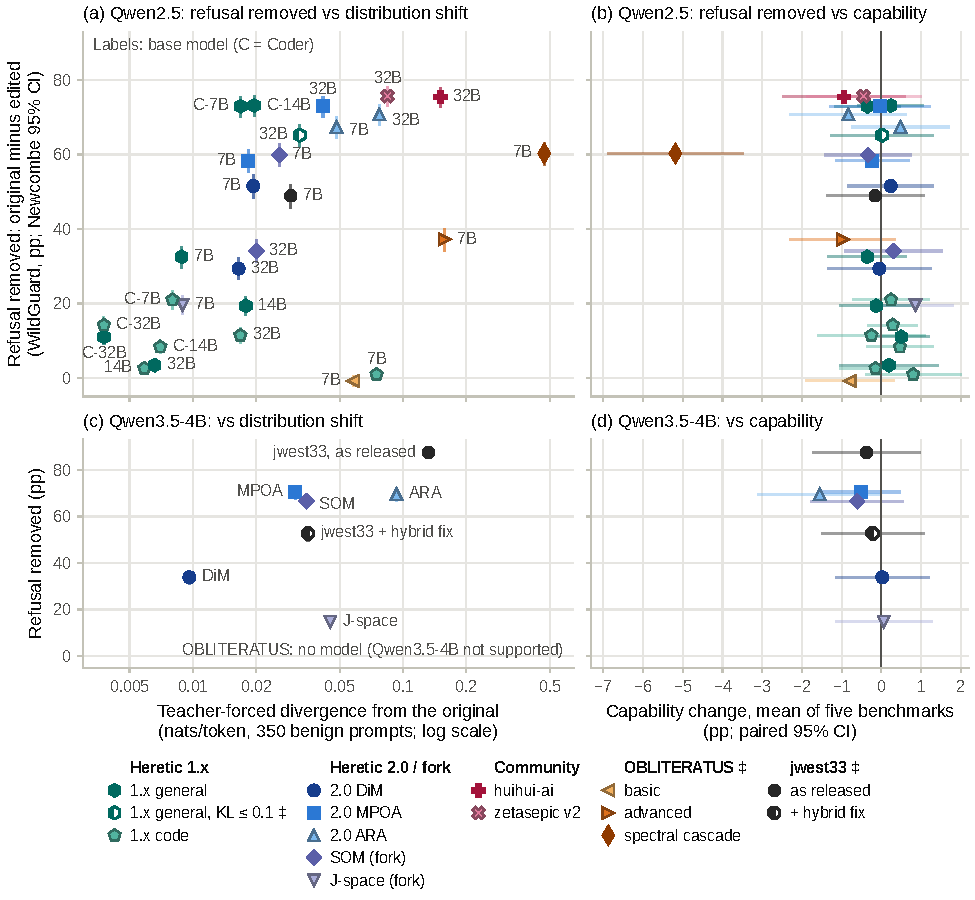
\includegraphics[width=\textwidth]{figures/fig2_tradeoff.pdf}
\caption{\textbf{Refusal removed versus its cost.} Each marker is one edited model. The vertical axis is the paired
reduction in WildGuard residual refusal from the model's own original (Newcombe 95\% CI). (a, c) TF divergence from
the original on the 350 benign held-out prompts (log scale). (b, d) Change of the mean of the five capability
benchmarks, with paired 95\% intervals. (a, b) Qwen2.5 models, labelled by base model (C = Coder), including the
cells added after the main design ($\S$: the KL $\le$ 0.1 re-export and the external tools on Qwen2.5-7B, each
external preset run once at its default or recommended settings); the jwest33 marker in (a, b) is the Qwen2.5-7B
run, whose runtime patch has no effect on that non-hybrid model, so it is effectively the tool as released. (c, d)
Qwen3.5-4B: the companion study's seed-1 models and the two jwest33 runs (as released, primary; with the hybrid
fix, sensitivity run); OBLITERATUS v0.1.4 does not support this model. The within-model correlations quoted here
use the main-design cells only (eight edited models on Qwen2.5-32B, seven on Qwen2.5-7B). Within Qwen2.5-32B, refusal removed rises with TF divergence (Spearman $\rho=-0.93$ for residual refusal);
within Qwen2.5-7B it does not ($\rho=-0.18$, not significant), because 1.x code moved that model furthest among the
Heretic models without removing refusal. Across base models the same divergence corresponds to very different
reductions (for example 11.4 to 73.1~pp between 0.016 and 0.021 nats per token), and at equal divergence tools can
differ (2.0 DiM versus 1.x code on Qwen2.5-32B). No capability change of the main design differs from zero; among
the added cells only OBLITERATUS \texttt{spectral\_cascade} ($-$5.18~pp) has an interval that excludes zero.
``(fork)'' = project-fork plug-in.}
\label{fig:tradeoff}
\end{figure*}

% src (cells.csv overrefusal_wg_rate; tests_refusal.csv vs_base benign_all wg 21/23; hb_harm_rate 32B and 7B)
Over-refusal on the benign prompts fell in 21 of the 23 edited models (Holm-significant); the exceptions were the 1.x
code variants on Qwen2.5-7B and Qwen2.5-14B. Harmful compliance by the HarmBench classifier mirrored refusal: on
Qwen2.5-32B it rose from 19.8\% for the original to 22.1\% and 27.6\% for the two 1.x variants, 40.3\% for 2.0 DiM,
82.3\% for ARA, 85.3\% for MPOA and 90.1\% and 91.0\% for the community releases; on Qwen2.5-7B from 23.3\% to 25.5\%
(1.x code), 45.6\% (1.x general) and 36.3\% to 79.0\% for the 2.0 and fork models.

\subsection{Search Records and the Selection Cap (Exploratory)}

% src (RESULTS.md "Dev set at matched KL caps"; dev_matched_kl.csv; correlations.csv dev_refusals_general~wg_rate
%      +0.95 [0.82, 1.00] n=15; cells.csv dev_refusals)
This section uses the optimisation records, not the held-out harness. Its counts are keyword refusals on the 100
dev prompts, scored during each search under that search's own settings: the 1.x searches used the
coding-assistant system prompt and 32 markers, the 2.0 and fork searches the generic system prompt and 33 markers
(Table~\ref{tab:h1setup}), so dev counts from the two versions are not directly comparable. Table~\ref{tab:devkl} and
Figure~\ref{fig:devkl} show what each search could have released at other dev-KL caps. At the 1.x cap (KL $\le$ 0.01)
the 1.x general search on Qwen2.5-32B had reached 89 dev refusals of 100, against 94 for 2.0 DiM, 83 for MPOA and 96
for SOM, while ARA had no trial below that cap. At the 2.0 cap (KL $\le$ 0.1) the same 1.x search had reached 50
(trial~\#96, the trial re-exported in \S\ref{sec:res-kl}), against 89 for DiM, 73 for SOM, 13 for MPOA and 10 for
ARA. On Qwen2.5-7B the 1.x general search reached 67 dev refusals at KL $\le$ 0.01, 30 at KL $\le$ 0.02 (ARA: 10) and
7 at KL $\le$ 0.1 (ARA 8, MPOA 19, SOM 27, DiM 55, J-space 84). At the 2.0 cap the 1.x general searches on the other
four models had reached 5 (Qwen2.5-Coder-7B), 9 (Qwen2.5-Coder-14B), 12 (Qwen2.5-14B) and 22 (Qwen2.5-Coder-32B)
dev refusals. The selected trials had realised dev KL of 0.004 to 0.010 (1.x) and 0.018 to 0.078 (2.0 and fork
plug-ins). Across the 15 edited models scored on the general dev prompts, the dev refusal count of the selected trial
ranked held-out residual refusal closely (Spearman $\rho=+0.95$ [0.82, 1.00]), but this pooled correlation mixes the
two dev protocols and six base models. Within Qwen2.5-32B, the selected 1.x general and 2.0 DiM trials both had 89
dev refusals and left 73.4\% and 47.4\% held-out residual refusal, and the re-exported 1.x trial with 50 dev
refusals left 11.6\%; within Qwen2.5-7B, the 1.x general and DiM trials had 67 and 55 dev refusals and left 39.6\%
and 20.6\%. Apart from trial~\#96, the held-out behaviour of unselected 1.x trials was not measured.

\begin{figure*}[tbp]
\centering
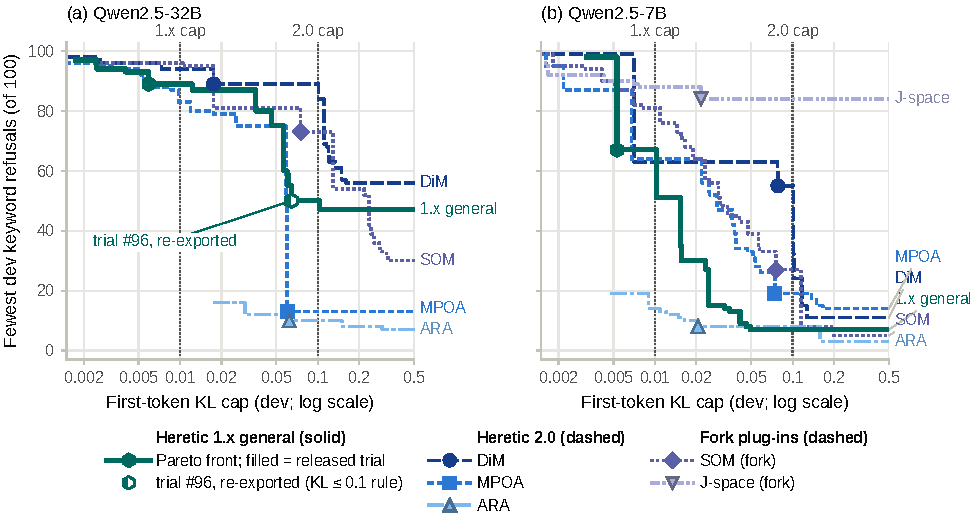
\includegraphics[width=\textwidth]{figures/fig4_dev_kl_budget.pdf}
\caption{\textbf{What each search could have released at a given dev-KL cap (search records; exploratory).}
Fewest keyword refusals among the 100 \texttt{harmful\_behaviors} dev prompts reached by any trial whose
first-token KL divergence is at or below the cap, for the Heretic~1.x general search (Pareto front of 200 trials,
seed~0) and the Heretic~2.0 and fork-plug-in searches (all 100 trials, seed~1). Dev counts were scored during each
search under its own settings (1.x: ``You are a helpful coding assistant.'', 32 markers; 2.0: ``You are a helpful
assistant.'', 33 markers), so the 1.x and 2.0 curves are not on a common scale. Filled markers: the released trial
(1.x: KL $\le$ 0.01 rule of the archived runs; 2.0 and fork: KL $\le$ 0.1 rule of the companion study); half-filled
hexagon in (a): 1.x trial~\#96, the trial that the KL $\le$ 0.1 rule selects, re-exported (\S\ref{sec:reexport}).
The 1.x code variant used a different dev set and is not shown. No held-out data enter this figure; the held-out
result of trial~\#96 is reported in \S\ref{sec:res-kl}.}
\label{fig:devkl}
\end{figure*}

\begin{table}[tbp]
\centering\small
\caption{Fewest dev keyword refusals (of 100 \texttt{harmful\_behaviors} test prompts) reachable at each
first-token KL cap, from the optimisation records (1.x: Pareto front; 2.0 and fork plug-ins: all trials);
``Selected'' is the released trial. Counts were scored under each search's own system prompt and marker list
(Table~\ref{tab:h1setup}) and are not directly comparable between 1.x and 2.0. -- = no trial at or below the cap.}
\label{tab:devkl}
\setlength{\tabcolsep}{4pt}
\resizebox{\textwidth}{!}{\begin{tabular}{@{}llrrrrrr@{}}
\toprule
Model & Search & Selected: refusals (KL) & \multicolumn{5}{c}{Fewest dev refusals at first-token KL $\le$} \\
\cmidrule(l){4-8}
 & & & 0.01 & 0.02 & 0.05 & 0.1 & 0.5 \\
\midrule
Qwen2.5-7B & 1.x general & 67 (0.005) & 67 & 30 & 7 & 7 & 7 \\
 & 2.0 DiM & 55 (0.078) & 63 & 63 & 63 & 55 & 11 \\
 & 2.0 MPOA & 19 (0.074) & 64 & 64 & 33 & 19 & 14 \\
 & SOM (fork plug-in) & 27 (0.076) & 81 & 64 & 39 & 27 & 5 \\
 & J-space (fork plug-in) & 84 (0.022) & 88 & 88 & 84 & 84 & 84 \\
 & 2.0 ARA & 8 (0.021) & 14 & 10 & 8 & 8 & 3 \\
\addlinespace[2pt]
Qwen2.5-Coder-7B & 1.x general & 21 (0.010) & 21 & 5 & 5 & 5 & 5 \\
\addlinespace[2pt]
Qwen2.5-14B & 1.x general & 91 (0.008) & 91 & 91 & 25 & 12 & 3 \\
\addlinespace[2pt]
Qwen2.5-Coder-14B & 1.x general & 36 (0.010) & 36 & 14 & 9 & 9 & 9 \\
\addlinespace[2pt]
Qwen2.5-32B & 1.x general & 89 (0.006) & 89 & 87 & 75 & 50$^{a}$ & 47 \\
 & 2.0 DiM & 89 (0.018) & 94 & 89 & 89 & 89 & 56 \\
 & 2.0 MPOA & 13 (0.060) & 83 & 79 & 75 & 13 & 13 \\
 & SOM (fork plug-in) & 73 (0.075) & 96 & 81 & 81 & 73 & 30 \\
 & 2.0 ARA & 10 (0.062) & -- & 16 & 12 & 10 & 7 \\
\addlinespace[2pt]
Qwen2.5-Coder-32B & 1.x general & 94 (0.007) & 94 & 86 & 74 & 22 & 4 \\
\bottomrule
\multicolumn{8}{@{}l}{\footnotesize $^{a}$ Trial \#96 (KL 0.064), re-exported and evaluated held-out (Table~\ref{tab:h1}b);} \\
\multicolumn{8}{@{}l}{\footnotesize \phantom{$^{a}$} dev re-evaluation after export: 51 of 100 at KL 0.064.} \\
\end{tabular}
}
\end{table}

\subsection{Summary of Findings}

The twelve Heretic~1.x models removed between 0.9~pp (not significant) and 73.1~pp of judged refusal, depending on
the base model and the direction source, with no detectable capability cost. In the pre-stated like-for-like
contrast, 2.0 DiM left less residual refusal than 1.x general on both base models (25.9~pp on Qwen2.5-32B, 19.0~pp
on Qwen2.5-7B), so H1 was supported as stated for the released checkpoints. When the archived 1.x general search on
Qwen2.5-32B was re-exported at the 2.0 selection rule, the 1.x model left 11.6\% of the harmful prompts refused:
61.7~pp less than the released export of the same search and 35.8~pp less than 2.0 DiM, at a TF divergence of 0.032
nats per token and without a detectable capability change; on that model only MPOA, ARA and the two community
releases left less. With both arms selected by the same rule, the like-for-like gap on Qwen2.5-32B therefore did not
persist (one search per arm; no such test exists for Qwen2.5-7B). A code-derived
direction gave no consistent advantage on malicious-code prompts in any of the six models (H2 not supported).
Keyword matching counted more refusals than the judge after strong edits, also within the first 256 tokens; within
the main design it rarely changed the order of tools, but among the external-tool contrasts it reversed one
significant difference (H3 partially supported). Of the external tools, each run once at its own default or
recommended settings, OBLITERATUS
\texttt{basic} removed no refusal, \texttt{advanced} removed 37.2~pp and \texttt{spectral\_cascade} 60.3~pp, the
latter with the only significant capability loss and the most degenerate responses in the study; jwest33's
abliterator removed 48.9~pp on Qwen2.5-7B and, as released, 87.4~pp on Qwen3.5-4B (52.7~pp with the
hybrid-architecture detection restored). Within Qwen2.5-32B, refusal removed tracked TF divergence closely; within
Qwen2.5-7B it did not.

% =====================================================================
% 5 DISCUSSION (purpose + finding | figures in order | novelty + hypotheses | confounds | literature | limitations)
% Revised 2026-11-06: H1 = like-for-like; efficiency statement restricted to within-model evidence; keyword-256 used
% for the H3 mechanism; v1 Yi inference removed; fork plug-ins labelled.
% Revised 2026-11-06 (draft v3): 7B 1.x cells, KL<=0.1 re-export (selection-cap check now answered), external tools.
% "Suggest, but do not establish" removed; no claim that every 2.0 configuration beats 1.x (7B J-space does not;
% at matched cap 1.x beats 2.0 DiM and SOM on 32B). Sources (analysis/, assemble_p30.py run 2026-11-06T22:47Z):
%   cells.csv (rates, CIs, TF divergence, capability mean delta, dev/re-eval counts, ext_* self-reports,
%   degenerate_rate); tests_refusal.csv families vs_base, h1_1x_vs_2.0, h2_general_vs_code, kw_vs_judge,
%   within_model_pairs (original design) and vs_base_added, h1_kl_matched, kl_cap_1x, external_vs_heretic,
%   external_sensitivity, kw_vs_judge_added (added); tests_capability.csv (family original_design / added);
%   correlations.csv (pooled, 23 edited main-design cells); dev_matched_kl.csv; rank_flips.csv;
%   reexport_1x/results_rtx/*/PROVENANCE.json (validation gate). Paper-33 numbers (seed-noise threshold, 7B DiM
%   seed 2) cited to the companion study.
% NOTE (checked 2026-11-06 after supp_stats.py re-run at 15:03 on the current analysis outputs): supp_stats.csv
%   spearman_wg_tf_within_qwen2.5-32b -0.9286 (n=8, exact permutation p=0.0022; re-derived from cells.csv);
%   within qwen2.5-7b -0.1786 (n=7, p=0.7131; not quoted, the 7B statement below is descriptive from cells.csv);
%   kw_gap_shrink_full_to_256_median_pp 2.37 (n=23, range 0.3--5.6; re-derived from tests_refusal.csv kw_vs_judge,
%   kw_minus_wg minus kw256_minus_wg); edited_kw_only_capped_share 0.4464, edited_wg_comply_capped_share 0.5719.
%   Seed-noise threshold 25.9 pp [18.1, 45.4] (2 x SD_diff 12.9) and 7B DiM seed 2 = 4.4%: paper 33
%   results/analysis/seednoise_summary.md and final_seed_generation.csv.
% =====================================================================
\section{Discussion}
\label{sec:discussion}

This study rebuilt archived Heretic~1.x models and compared them, on held-out prompts with a validated judge, with
Heretic~2.0, two project-fork plug-ins, two external tools run at their documented settings and two community
releases on the same base models. The twelve 1.x models removed between 0.9~pp (not significant) and 73.1~pp of
refusal, depending on the base model and the direction source. In the like-for-like contrast, the same edit released
by Heretic~2.0 left 25.9~pp less residual refusal than when released by 1.x on Qwen2.5-32B and 19.0~pp less on
Qwen2.5-7B, so H1 was supported as stated. The check of the selection cap reversed the reading of that result:
released from the same Qwen2.5-32B search under the 2.0 rule, the 1.x model left 35.8~pp less residual refusal than
2.0 DiM. On that model, the advantage of the newer version under the archived settings therefore reflects the rule
that selected the released trial, not the version; on Qwen2.5-7B the same check was not run. For a practitioner, the selection rule and the divergence at which a tool
releases its output matter at least as much as the tool's version, and external tools run at their documented
settings ranged from no effect on refusal to near-complete removal.
% src: RESULTS.md "Modified vs original" (0.9 = qwen2.5-7b 1.x code, p_Holm 0.222; 73.1 = coder-14b 1.x general);
% RESULTS.md "H1" (+25.9 [23.0, 28.7]; +19.0 [16.1, 21.9]); RESULTS.md "1.x general re-exported at KL <= 0.1"
% (-35.8 [-38.9, -32.7]).

The like-for-like contrast (Figure~\ref{fig:refusal}, Table~\ref{tab:h1}) was large and robust to the judge on both
base models, and the search records had already indicated where to look. The archived 1.x runs released the trial
with the fewest dev refusals at dev KL $\le$ 0.01, a cap ten times tighter than the companion study's 0.1. On
Qwen2.5-32B the released 1.x trial had kept 89 of 100 dev refusals, whereas the same search had reached 50 at dev KL
0.064 (Figure~\ref{fig:devkl}). Re-exported with heretic-llm 1.4.0, the release identified from the run records,
that trial left 11.6\% of the harmful prompts refused (\S\ref{sec:res-kl}, Table~\ref{tab:h1}b): 35.8~pp less than
2.0 DiM but 7.7 and 5.6~pp more than MPOA and ARA, at a TF divergence between those of DiM and MPOA and without a
measurable capability change. Each of these decisions held under keyword matching, under Qwen3Guard and without the
AdvBench-overlap prompts. With the cap equalised, the older version's search thus released
a model that removed more refusal than the newer version's DiM search, the reverse of the H1 contrast. This does not
show that 1.x is the better version. The arms still differ in trial budget (200 versus 100 trials), seed, system
prompt, marker list and the KL target of the 1.x objective, and at dev KL $\le$ 0.1 the 2.0 DiM search never went
below 89 dev refusals, so the reversal is as consistent with a weaker DiM search as with any property of the
version. On
Qwen2.5-7B, where no trial was re-exported, the 1.x general search had reached 7 dev refusals at KL $\le$ 0.1 against
55 for DiM; this points in the same direction, but on dev scales that are not directly comparable.
% src: dev_matched_kl.csv (32B 1x_general: selected 89 @ 0.0059, min_ref_kl0.1 = 50 @ 0.0642; 32B dim min_ref_kl0.1
% = 89 @ 0.0175, kl0.2 = 56 @ 0.160; 7B 1x_general kl0.1 = 7 @ 0.049, 7B dim selected 55 @ 0.078);
% RESULTS.md coverage row qwen2.5-32b__heretic1x-general-kl0.1 (heretic-llm 1.4.0, git v1.4.0 6ea3b8d; trial #96);
% tests_refusal.csv kl_cap_1x (-61.7 [-64.7, -58.5]) and h1_kl_matched (DiM -35.8 [-38.9,-32.7]; SOM -31.1
% [-34.0,-28.1]; MPOA +7.7 [5.9, 9.7]; ARA +5.6 [3.6, 7.6]; all p_Holm<0.001 for wg, kw, q3g, harmful_all and
% harmful_excl_advbench); cells.csv tf_divergence (kl0.1 0.0323, dim 0.0165, mpoa 0.0416), capability_mean_delta
% (+0.02 [-1.27, +1.31]); 04_methods tab:h1setup (budget, seed, prompt, markers, KL target).

Not every newer configuration removed more refusal than 1.x. On Qwen2.5-32B, only MPOA and ARA, which also change
the edit, left less held-out refusal than the KL-matched 1.x model (they had reached 13 and 10 dev refusals at the
2.0 cap), by 7.7 and 5.6~pp. Both differences are well below the companion study's seed-noise threshold of
25.9~pp \cite{young2026harder}, so the order of these three models could change with another search seed. On
Qwen2.5-7B, J-space (fork plug-in) left 13.0~pp [10.3, 15.6] more residual refusal than 1.x general. The external
tools, each run once at its documented default or recommended settings without a search or selection cap, spanned
the whole range of outcomes (\S\ref{sec:res-external}, Table~\ref{tab:external}). OBLITERATUS's \texttt{basic}
preset did not change residual refusal on Qwen2.5-7B, and the tool's own check, which reported 83\% refusal on its
prompts, agreed, so the null result reflects the preset, not the harness. Its \texttt{spectral\_cascade} preset left
the least refusal of the external presets on that model, but at the largest TF divergence of any cell, with the most
degenerate responses and the only per-benchmark loss in the study that survived Holm correction. Qwen2.5-7B is not a
hybrid model, so the restored hybrid-architecture detection had no effect on jwest33's run there, which is
effectively the tool as released; it did not differ significantly from 2.0 DiM after Holm correction. On the
hybrid-attention Qwen3.5-4B, the tool as released left 1.0\% of the harmful prompts refused, less than every
Heretic configuration evaluated there, whereas the run with the detection restored, which differs only in that
detail, left 35.8\%, a difference of 34.8~pp [31.8, 37.8]. Each
of these cells describes one preset of one tool in a single run; together they show how strongly the outcome depends on the preset and on
architecture handling, not which algorithm is better.
% src: dev_matched_kl.csv (32B mpoa 13 @ 0.060, ara 10 @ 0.062); tests_refusal.csv h1_kl_matched (kl0.1 vs mpoa
% +7.7, vs ara +5.6; vs dim/som negative); seed-noise threshold 25.9 pp: see header note; h1_1x_vs_2.0 (7B 1.x general vs
% jspace -13.0 [-15.6, -10.3], p_Holm<0.001); vs_base_added (obliteratus-basic +0.8 [-0.6,+2.3], p_Holm 0.332);
% cells.csv ext_self_refusal_rate (basic 0.833), wg_rate (advanced 35.0, spectral 11.8, jwest33 7B 23.3, 4B 1.0
% [0.6, 1.9] / 35.8), tf_divergence (spectral 0.4709 = max over all cells; 4B as released 0.1322, hybrid fix
% 0.0353), degenerate_rate (spectral 56/972; RESULTS.md "Anomalies"), ext_hybrid (7B False, 4B True),
% ext_runtime_patches; tests_capability.csv family added (spectral mmlu_pro -7.0 [-9.93,-4.05], p_Holm 0.0003;
% no other test of either family p_Holm<0.05; mean5 -5.18 [-6.90,-3.47]); external_vs_heretic (jwest33 7B vs DiM
% +2.7 [0.3, 5.1], p_Holm 0.132; 4B as released vs dim/mpoa/som/jspace/ara all negative, p_Holm<0.001; hybrid fix vs
% dim -18.8, p_Holm<0.001); external_sensitivity (-34.8 [-37.8, -31.8]).

The source of the refusal direction mattered less than expected (Figure~\ref{fig:general-code}). The originals
already complied with most malicious-code requests, refusing only 13.5--34.0\% of them, so a code-specific
direction had little refusal to target, and in all six models the variant that left less residual refusal on one
subset left less or equal residual refusal on the other; on four of them (both 7B and both 14B models) the general
variant was lower on both. A largely shared refusal mechanism \cite{arditi2024refusal} would produce this pattern,
but the two variants did not differ simply in how far their searches moved the model: the code variant diverged less
than the general variant on three models and more on two, and on Qwen2.5-7B it diverged about eight times as far
(TF divergence 0.075 versus 0.009 nats per token) while leaving refusal unchanged ($-$0.9~pp [$-$2.3, +0.4]). A
shared mechanism was not tested directly, for example by comparing the two directions layer by layer or the two
variants at matched divergence. Coder checkpoints were not consistently easier or harder to edit: the general
variant removed 72.9 and 73.1~pp on Qwen2.5-Coder-7B and Qwen2.5-Coder-14B but 11.0~pp on Qwen2.5-Coder-32B.
% src: cells.csv wg_code_rate of originals (7B 13.5, coder-7B 32.0, 14B 17.0, coder-14B 34.0, 32B 16.1, coder-32B
% 18.5); RESULTS.md "H2" (code_weapon and harmful_noncode rows, 6 models); cells.csv tf_divergence of 1.x cells
% (code < general: coder-7B, 14B, coder-14B; code > general: 7B 0.0749 vs 0.0089, 32B 0.0168 vs 0.0066; equal:
% coder-32B 0.0038); RESULTS.md "Modified vs original" (7B 1.x code -0.9 [-2.3,+0.4]; coder-7B general -72.9;
% coder-14B general -73.1; coder-32B general -11.0).

Keyword counting changed the size of differences more than their order (Figure~\ref{fig:refusal}b). In the main
design keyword matching counted significantly more refusals than WildGuard in 15 of 23 edited models and fewer in
none, by up to 19.5~pp; one of 76 within-model pairs changed sign between the two measures, a pair that differed
significantly under keyword matching only, and every 1.x-versus-2.0 decision was the same under both. Keyword
reports would therefore understate the reductions achieved by the strongest edits relative to either judge. The
direction of the gap is not fixed, however: among the added cells keyword matching counted 16.6~pp more refusals
than WildGuard for the KL-matched 1.x model but 21.1~pp fewer for J-space on Qwen3.5-4B. The data show disagreement
between keyword matching and the judges, not which of them is correct, and the correlation of the gap with the
refusal removed is partly mechanical, because as judged refusal approaches zero the only possible disagreements are
keyword flags on answers the judge counts as compliant. In the companion study the gap was concentrated in responses
that reached the 512-token limit \cite{young2026harder}. Here, restricting keyword matching to the first 256 tokens
removed a median of only 2.4~pp of the gap, and keyword-only refusals had reached the limit less often than the
responses WildGuard counted as compliant, so on these models the gap is not explained by long responses alone;
safety vocabulary early in otherwise compliant answers, such as warnings and disclaimers, is a plausible source that
a human audit could confirm. The re-exported 1.x model shows the same problem one step earlier, in the search
itself. Trial~\#96 had kept 50 of 100 dev refusals by keyword count, yet on the held-out prompts it left 28.2\%
refused by keyword count and 11.6\% by WildGuard. On identical held-out responses keyword matching accounted for
16.6~pp [13.4, 19.7] of that difference; the remainder reflects differences between the dev protocol
(AdvBench-derived prompts, the coding-assistant system prompt, 100-token responses and the 1.x marker list) and the
held-out one. Equal dev counts were equally uninformative: the two released Qwen2.5-32B trials of the like-for-like
contrast both had 89 dev refusals, each under its own arm's protocol, and left 73.4\% and 47.4\% held-out refusal.
% src: tests_refusal.csv kw_vs_judge, kw_minus_wg, harmful_all, 23 edited main-design cells: 15 p_Holm<0.05 with
% diff>0, 0 with diff<0, max +19.5 (qwen2.5-7b DiM); RESULTS.md "Within-model order flips" (1 of 76; 0 significant
% under WG with opposite sign); rank_flips.csv (huihui vs zetasepic: WG +0.2 n.s., kw -4.6 p_Holm<0.001);
% h1_1x_vs_2.0 kw: all 18 significant, same sign as wg; kw_vs_judge_added (kl0.1 +16.6 [13.4, 19.7]; qwen3.5-4b
% jspace -21.1, p_Holm<0.001); keyword-256 median shrink: see header note; capped shares: supp_stats.csv
% edited_kw_only_capped_share 0.4464 vs edited_wg_comply_capped_share 0.5719 (23 edited main-design cells,
% 22,356 harmful responses); cells.csv kl0.1: dev_refusals 50
% (journal; re-eval 51), kw_rate 28.2, wg_rate 11.6; 1.x dev protocol: 04_methods (system prompt, 100 tokens,
% 32 markers); dev_matched_kl.csv selected 89/89; RESULTS.md H1 rows.

Within Qwen2.5-32B the ranking of tools largely followed how far they moved the model (Figure~\ref{fig:tradeoff}):
residual refusal fell almost monotonically with TF divergence across the eight edited models of the main design
(Spearman $\rho=-0.93$, exact permutation $p=0.002$), the KL-matched 1.x model fell into the same ordering (11.6\% at 0.032 nats per token,
between SOM and MPOA), and the community releases sat at its far end (0.085 and 0.151 nats per token). The ordering
did not hold on Qwen2.5-7B: the 1.x code variant moved the model further than any other Heretic configuration on that
model (0.075 nats per token) without changing refusal, and OBLITERATUS \texttt{basic} diverged by 0.058 without
changing it either. Across the 23 edited models of the main design residual refusal still fell as TF divergence rose
(Spearman $\rho=-0.75$ [$-$0.93, $-$0.38]), but the same divergence corresponded to very different reductions on
different base models, and on one model tools differed at equal divergence (on Qwen2.5-32B, 2.0 DiM left 17.9~pp
less residual refusal than 1.x code, both at 0.017). Divergence is therefore a cost an edit pays, not a
model-independent measure of what it buys. Capability benchmarks registered little of this. In the main design no
per-benchmark change survived correction and the mean changes stayed within one point, although models that removed
more refusal tended to lose slightly more (Spearman $\rho=+0.50$ [0.08, 0.79] between residual refusal and mean
change). The one clear loss accompanied the largest divergence in the study, OBLITERATUS \texttt{spectral\_cascade}
at 0.471 nats per token. At the divergences reached by the Heretic searches, TF divergence on benign prompts is
therefore a more sensitive indicator of what an edit changes than the five benchmarks, although the absence of
significant benchmark changes reflects limited power as well as small effects. The earlier comparison's 18.8-point
GSM8K loss for Heretic on Yi-1.5-9B \cite{young2025comparative} has no counterpart among the Qwen2.5 models here; no
Yi model was evaluated, so the two results do not conflict.
% src: supp_stats.csv spearman_wg_tf_within_qwen2.5-32b (-0.9286, n=8, exact permutation p=0.0022; see header note;
% with the KL-matched cell added_spearman_wg_tf_within_qwen2.5-32b_incl_kl01 -0.95, n=9, p=0.0004);
% cells.csv tf_divergence / wg_rate (32B: som 0.0202/42.7, kl0.1 0.0323/11.6, mpoa 0.0416/3.9, zetasepic 0.0847,
% huihui 0.1511; 7B: 1.x code 0.0749/71.2 > ara 0.0484, obliteratus-basic 0.0579/72.9); correlations.csv (wg_rate
% vs tf_divergence n=23 -0.75 [-0.93,-0.38]; wg_rate vs capability_mean_delta_pp n=23 +0.50 [0.08, 0.79], p=0.016);
% within_model_pairs (32B dim vs 1.x code); tests_capability.csv original_design (no p_Holm<0.05; mean deltas
% -0.94 to +0.86).

To the best of current knowledge this is the first held-out, judge-based comparison of two versions of the same
abliteration tool in a documented like-for-like setup that also releases the older version's search under the newer
version's selection rule, of general- versus code-derived refusal directions, and of Heretic output against external
tools and public community releases on the same checkpoints. H1 was supported on both base models on which both
versions were judged, but on Qwen2.5-32B the KL-matched check showed that the support reflects the archived
selection cap rather than the version; on Qwen2.5-7B the difference (19.0~pp) is below the companion study's
seed-noise threshold of 25.9~pp [18.1, 45.4], and the companion study's second seed of the same DiM configuration
left 4.4\% instead of 20.6\% \cite{young2026harder}. H2 was not supported, and H3 was partially supported, because the
keyword--judge gap was tool-dependent but rarely reordered tools.

Several alternative explanations were examined. The like-for-like arms differ in trial budget, search seed,
optimisation system prompt, marker list and KL objective as well as in selection cap and version
(Table~\ref{tab:h1setup}). The KL-matched re-export removes the cap difference for one search and leaves the others,
so it shows that the cap alone suffices to reverse the Qwen2.5-32B contrast, not that it is the only setting that
matters. The re-export could itself have drifted from the archived run; it was accepted only after re-exporting the
originally released trial with the same script had reproduced the archived adapter numerically
(\S\ref{sec:reexport}, Appendix~\ref{app:reexport}), and trial~\#96 reproduced its own record (51 versus 50 dev
refusals). The eight rebuilt 14B and 32B
1.x models were tensor-for-tensor identical to the archived merges; for the four 7B 1.x models no archived tensor
hashes exist, but their adapters matched their manifests. Within each base model all cells were generated with
identical decoding, prompts and judges; the one harness difference, for the Qwen2.5-32B original, affects its MBPP
comparisons, which are unpaired, and output post-processing that changes nothing in its responses. Removing the 44
AdvBench-overlap prompts changed no decision of the main design or of the KL-matched check; among the external-tool
comparisons it changed one WildGuard decision (OBLITERATUS \texttt{advanced} versus 1.x general on Qwen2.5-7B,
$-$4.6~pp, no longer significant) and three Qwen3Guard decisions (the same pair, and \texttt{spectral\_cascade}
versus MPOA and versus SOM, which became significant). Removing the 41 code-as-weapon prompts drawn from the
code variant's source corpora removed the only evidence for a code-specific advantage. WildGuard has moderate
agreement with human labels \cite{xie2025sorrybench}, but Qwen3Guard reproduced every 1.x-versus-2.0 decision and
every decision of the KL-matched check. SOM and J-space are plug-ins of the companion study's fork, so their
contrasts describe configurations that a Heretic~2.0 user does not obtain from a release. Finally, 19 of the 42
judged cells were first reported in the companion study; they serve here as comparators, and the hypotheses concern
the new 1.x cells.
% src: reexport_1x/results_rtx/trial84_validation_records/PROVENANCE.json (validation: n_edited 62/62,
% min_direction_cosine 0.99998761, reeval 90, reevaluated_original_adapter_here 90, journal 89; verdict "PASS
% (numerically equivalent, not bit-identical)"); results_rtx/qwen2.5-32b__heretic1x-general-kl0.1/PROVENANCE.json
% (journal 50 @ 0.0642, re-eval 51 @ 0.0637); cells.csv tensors_* / adapter_sha256_ok (7B 1.x: True, no tensor
% hashes; RESULTS.md coverage "tensor hashes not available"); tests_refusal.csv harmful_all vs
% harmful_excl_advbench decisions (re-checked over all families x wg/kw/q3g: changes only in external_vs_heretic,
% 1 wg + 3 q3g, 0 kw: advanced vs 1.x general wg -4.6 p_Holm 0.017 -> 0.154, q3g 0.007 -> 0.064; spectral vs mpoa
% q3g 0.109 -> 0.012 and vs som q3g 0.113 -> 0.037); h1_1x_vs_2.0 and
% h1_kl_matched q3g (all significant, same sign as wg); cells.csv provenance (19 companion cells: 7B x6, 32B x7,
% qwen3.5-4b x6; 42 judged).

The results agree with reports that susceptibility to abliteration is model-specific rather than a function of
size \cite{hadetskyi2026not}: the same 1.x procedure removed 3.4~pp from Qwen2.5-32B and 73.1~pp from
Qwen2.5-Coder-14B. They extend the companion study's observation that public releases reach lower refusal at larger
divergence \cite{young2026harder}: on Qwen2.5-32B the archived output of an older tool lies at the low-divergence end
of the same within-model ordering, and the same search, released at the newer cap, moves into its middle. They also
qualify the earlier tool ranking \cite{young2025comparative}, which ran each tool at its defaults and so mixed
algorithm, preset and selection rule; here the three presets of one tool left between 11.8\% and 72.9\% of the
harmful prompts refused on the same model, nearly as wide a range as the Heretic configurations and the other
external tool spanned together (4.7--71.2\%). The jwest33 result on Qwen3.5-4B adds that architecture support is
part of a tool's behaviour: on hybrid-attention models, whether a code path detects the architecture can matter as
much as the choice of method.
% src: RESULTS.md "Modified vs original" (32B 1.x general -3.4; coder-14B 1.x general -73.1); cells.csv wg_rate on
% qwen2.5-7b (obliteratus 72.9 / 35.0 / 11.8; Heretic + jwest33 4.7--71.2).

% Revised 2026-11-06: external-tool scope (OBLITERATUS: Qwen2.5-7B only; jwest33: + Qwen3.5-4B); seed caveat with
% the companion study's replicates.
% Revised 2026-11-06 (draft v3): the selection-cap re-export is done (the "needs a GPU run" TODO is resolved); its remaining
% limits stated (one study, one seed, one model, one cap, general direction only; code study not re-exportable because
% its prompt files are missing: reexport_1x/VERSION.md "Inputs not in /data"); external tools no longer pending;
% jwest33 Qwen3.5-4B: as-released run primary, hybrid-detection run sensitivity (author decision); 7B 1.x cells judged.
\subsection{Limitations and Future Work}
\label{sec:limitations}

The evidence is narrower than the question. All base models of the main design are from one family (Qwen2.5), the
like-for-like contrast rests on two base models, and Heretic~2.0 was not run on Qwen2.5-14B or the coder models. The
selection-cap check rests on a single re-exported trial: one search with one seed on one model (Qwen2.5-32B), for the
general direction only and at one cap (dev KL $\le$ 0.1). The 1.x code study could not be re-exported because its
prompt files were not archived with the run records, the Qwen2.5-7B searches and intermediate caps were not re-exported, and the
re-exported arm still differs from 2.0 DiM in trial budget, seed, system prompt, marker list and KL objective. The
external tools were each run once at their documented default or recommended settings, without a search or a
selection cap, so each cell describes one preset of one tool at an uncontrolled divergence rather than the best that
tool can do. OBLITERATUS was evaluated on Qwen2.5-7B only, because it does not support Qwen3.5-4B, and jwest33's
abliterator on Qwen2.5-7B and on Qwen3.5-4B, where the run as released is the primary cell and the run with the
restored hybrid-architecture detection a sensitivity analysis; the Qwen3.5-4B comparison lies outside the main
design and uses the companion study's Heretic~2.0 cells. Both tools' prompt pools partly overlap the held-out set
(\S\ref{sec:external}). ErisForge, llm-abliteration and FailSpy are represented only by the keyword-based results of
the earlier comparison. Each configuration contributed one search or run with one seed per model, so every test
compares two released checkpoints, and differences of the size of the companion study's seed-to-seed variation (a
standard deviation of about 13~pp for the difference between two independently optimised cells
\cite{young2026harder}) cannot be attributed to the tool or version with confidence. Responses were greedy and
limited to 512 tokens, so refusal later in long answers and sampling effects are not captured. Residual refusal
measures willingness, not the usefulness of a harmful answer; the HarmBench classifier's compliance label is only a
proxy \cite{carleo2026willing}. No human audit of the judged responses was done, so every rate is
relative to the automatic judges; an audit of a stratified sample is left to future work. The 1.x code variant's prompt files could not
be recovered (only the size of its dev set, 100 prompts, is recorded), so its overlap with the held-out code prompts was bounded by excluding all 41
prompts from the same corpora rather than checked item by item. The procedures behind the community releases are
undocumented.

Five next steps follow directly. Re-exporting the archived 1.x trials at intermediate caps (dev KL 0.02 and 0.05) on
Qwen2.5-32B and at the 2.0 cap on Qwen2.5-7B, and recovering the code study's prompt files so that its trials can be
re-exported, would show how the held-out effect of the cap scales and whether it holds beyond one search. Running the
2.0 DiM search with the 1.x trial budget, seed, system prompt and marker list, or the reverse, would separate these
settings from the version once the cap is matched. A second search seed per arm, starting with the companion study's
existing seed-2 Qwen2.5-7B cells, would show how much of each contrast exceeds search-to-search variation. Running
the external tools across their documented settings, and at a divergence cap where the tool allows one, would
separate preset from algorithm, and adding at least one non-Qwen family would test generality. Releases of
abliterated models should state the selection rule and the divergence at which they were selected.


% Revised 2026-11-08 (ARS review): R3 selection-rule framing; R4 causal attribution scoped to one Qwen2.5-32B search
% with the remaining differences named; R6 single-case scope of the recommendation; R8 "one search per arm" and
% search-level verdict; R9 divergence named in the recommendation; R14 range at the archived cap; S4 Qwen3.5-4B
% outside the main design; S6 H2 as a pipeline; S8 "equivalent within +-2 pp" instead of "no detectable cost".
% Sources: RESULTS.md "Modified vs original", "H1", "1.x general re-exported at KL <= 0.1"; tests_refusal.csv
% kl_cap_1x, h1_kl_matched, h2_general_vs_code, kw_vs_judge; analysis/revision_20261108/h1_vs_threshold.csv,
% capability_equivalence.csv (12 1.x cells equivalent), dev_matched_divergence.csv; cells.csv (jwest33 Qwen3.5-4B
% wg 1.0, capped 87.8; obliteratus-basic 72.9).
\section{Conclusion}
\label{sec:conclusion}

All refusal rates below come from automatic judges without human audit. Judged on held-out prompts and selected at
the archived dev-KL cap of 0.01, Heretic~1.x models removed between 0.9
and 73.1~pp of refusal from six Qwen2.5 models, with capability changes equivalent to zero within $\pm$2~pp. With one
search per arm, Heretic~2.0 DiM left 25.9~pp less residual refusal than 1.x on Qwen2.5-32B and 19.0~pp less on
Qwen2.5-7B, differences significant for these checkpoints but inconclusive at the search level. In a post hoc
re-export of one Qwen2.5-32B 1.x search at the 2.0 cap, equalising the cap alone moved residual refusal from 73.4\% to
11.6\% and reversed the version contrast for these checkpoints, by an amount inside the interval of the seed-noise
threshold, while trial budget, seed, search range, objective, system prompt and marker list still differed and the re-exported model had moved about twice as far from the original as 2.0 DiM; the reversal is as
consistent with a weaker DiM search as with any property of the version. External tools run once at their documented
settings ranged from no change in refusal (OBLITERATUS \texttt{basic}) to near-complete removal on the hybrid
Qwen3.5-4B, outside the main design (jwest33's abliterator as released, with most responses running to the length
limit). The code pipeline gave no consistent advantage on malicious-code prompts, and keyword counts differed from
judged refusal after strong edits but rarely changed the order of tools. On the evidence of this single case,
comparisons and robustness assessments of abliteration tools should report the selection rule and the realised
divergence of the released model, use a judge on held-out prompts, and compare tools at matched divergence or across
the refusal--divergence trade-off rather than at one cap.


\section*{Ethics Statement}
% 2026-11-07: final text (author decisions: merged Heretic 1.x models are released; OpenRAIL++-M on own code, data and the
% Apache-2.0-based models; Heretic fork stays AGPL-3.0). src: analysis/cells.csv (wg_rate of every judged heretic1x cell
% vs the lowest public heretic2/community cell on the same base: 7B 1.x 39.6/71.2 vs 2.0 ARA 4.7; 32B 1.x 73.4/65.3/11.6
% vs zetasepic-v2 1.1; Coder-7B 10.3/62.2, 14B 58.2/75.0, Coder-14B 12.3/77.2, Coder-32B 64.3/61.1: no public model evaluated).
The study involved no human participants and no personal data and was not human-subjects research, so no IRB review
was required. It evaluates, and releases, language models whose refusal behaviour has been reduced, which is
dual-use. The marginal risk of the release is limited. On Qwen2.5-7B and Qwen2.5-32B, a model that was already
public before this study refused fewer held-out harmful prompts than every Heretic~1.x model released here (the
companion study's ARA model on Qwen2.5-7B, 4.7\%, and a community release on Qwen2.5-32B, 1.1\%;
Table~\ref{tab:cells}). For the four other bases (Qwen2.5-Coder-7B, Qwen2.5-14B, Qwen2.5-Coder-14B and
Qwen2.5-Coder-32B) no public abliteration was evaluated, so the argument does not extend to them; the most effective
1.x models there left 10.3\% and 12.3\% of harmful prompts refused. Outputs of the external tools are not released;
they can be regenerated from the pinned tool versions. Responses to harmful prompts are stored privately for scoring
and are not released. Released models keep the licence and use policy of their base model; models whose base is
licensed under Apache-2.0 additionally carry the use restrictions of the OpenRAIL++-M licence.

\section*{Data and Code Availability}
% 2026-11-07: final text. Repository created for both papers; Zenodo DOI is added when the first release is archived.
Code, configurations and data are at \url{https://github.com/ricyoung/abliteration-studies}: the evaluation harness,
the analysis and figure scripts (\texttt{assemble\_p30.py}, \texttt{make\_tables.py}, \texttt{make\_figures.py}),
the Heretic~1.x selection-cap re-export script with its provenance and validation records
(Appendix~\ref{app:reexport}), the external-tool run records (Appendix~\ref{app:external}), and the judge, keyword
and degeneracy labels of every held-out response, without prompt or response text. The 19 cells first reported in the
companion study \cite{young2026harder} (the 13 marked in Table~\ref{tab:cells} and the six Qwen3.5-4B context cells
of Table~\ref{tab:external}) share their response files and labels with that study. The rebuilt Heretic~1.x models
and the model re-exported at the 2.0 selection rule are on Hugging Face under
\url{https://huggingface.co/richardyoung}, together with their LoRA adapters and per-shard SHA-256 hashes. The
Heretic fork is at \url{https://github.com/ricyoung/heretic} under AGPL-3.0, the licence of upstream Heretic; the
code and data of this study are released under OpenRAIL++-M. \todo{Zenodo DOI of the archived release}

\bibliographystyle{unsrt}
\bibliography{references}

\newpage
\appendix
% =====================================================================
% APPENDIX (revised 2026-11-06: fork labels, 32B-original harness note, 1.x settings check, external tools,
% prior-work section for the new arXiv paper)
% Revised 2026-11-06 (pm): all 42 cells judged; "Pending cells" section removed; new sections app:reexport
% (selection-cap re-export provenance and validation) and app:external (external-tool provenance).
% Revised 2026-11-08 (ARS review): new app:seednoise (R1); added-cell marker double dagger (S3); app:reexport notes the
% 2.0.0 MLP range (R12); app:versions states the division of claims with the companion study (R2).
% =====================================================================
\section{Capability per Benchmark}
\label{app:capability}

% src (tests_capability.csv family original_design: 23 cells x 5 benchmarks, 0 Holm-significant; family added:
%      12 cells x 5, 1 Holm-significant (qwen2.5-7b__obliteratus-spectral_cascade mmlu_pro -7.0, p_holm 0.0003))
\begin{table}[!htbp]
\centering\footnotesize
\caption{Capability per benchmark. Rows ``Original'' give the original model's scores (\%); other rows
give the paired per-item change from that original (pp) and the change of the mean of the five benchmarks with a
95\% interval. None of the 115 per-benchmark changes of the main design is significant after Holm correction (exact
McNemar); of the 60 changes of the cells added after it ($^{\ddagger}$; separate Holm family), one is (bold: OBLITERATUS
\texttt{spectral\_cascade}, MMLU-Pro). $^{\dagger}$Unpaired comparison: the Qwen2.5-32B original was evaluated with an earlier harness revision
whose MBPP per-item samples predate the patched answer extractor; only its MBPP summary score was rescored from the
logged outputs, so its per-item scores are not available (\S\ref{sec:procedure}). SOM and J-space are plug-ins of
the companion study's project fork, not part of Heretic~2.0. One item is worth 0.1~pp (MMLU-Pro) to 0.61~pp
(HumanEval). The added cells are discussed in \S\ref{sec:res-kl} and \S\ref{sec:res-external}.}
\label{tab:capability}
\setlength{\tabcolsep}{4pt}
\resizebox{\textwidth}{!}{\begin{tabular}{@{}llrrrrrr@{}}
\toprule
Model & Condition & MMLU-Pro & GSM8K & IFEval & HumanEval & MBPP & Mean of five [95\% CI] \\
\midrule
Qwen2.5-7B & Original (score, \%) & 59.5 & 85.8 & 71.2 & 84.8 & 63.2 & 72.9 \\
 & 1.x general & +0.4 & $-$2.0 & $-$0.2 & $-$0.6 & +0.6 & $-$0.36 [$-$1.35, +0.63] \\
 & 1.x code & $-$1.4 & +3.2 & 0.0 & +0.6 & +1.6 & +0.80 [$-$0.41, +2.01] \\
 & 2.0 DiM & $-$1.4 & +0.2 & +0.6 & +1.2 & +0.6 & +0.23 [$-$0.85, +1.32] \\
 & 2.0 MPOA & $-$1.6 & $-$0.8 & $-$0.6 & +1.8 & 0.0 & $-$0.23 [$-$1.15, +0.70] \\
 & SOM (fork plug-in) & +0.3 & $-$1.8 & $-$0.6 & $-$1.2 & +1.6 & $-$0.33 [$-$1.44, +0.77] \\
 & J-space (fork plug-in) & +1.0 & +0.6 & +1.5 & 0.0 & +1.2 & +0.86 [$-$0.11, +1.82] \\
 & 2.0 ARA & $-$1.7 & +1.0 & $-$0.9 & +2.4 & +1.6 & +0.48 [$-$0.76, +1.72] \\
 & OBLITERATUS basic$^{\S}$ & $-$0.6 & +0.4 & $-$0.9 & $-$2.4 & $-$0.4 & $-$0.79 [$-$1.91, +0.33] \\
 & OBLITERATUS advanced$^{\S}$ & $-$3.4 & +1.2 & $-$2.2 & $-$1.8 & +1.4 & $-$0.97 [$-$2.30, +0.36] \\
 & OBLITERATUS spectral cascade$^{\S}$ & \textbf{$-$7.0} & $-$4.4 & $-$5.2 & $-$9.1 & $-$0.2 & $-$5.18 [$-$6.90, $-$3.47] \\
 & jwest33 recommended$^{\S}$ & $-$1.1 & $-$0.8 & +0.6 & $-$1.2 & +1.8 & $-$0.15 [$-$1.38, +1.08] \\
\addlinespace[2pt]
Qwen2.5-Coder-7B & Original (score, \%) & 41.6 & 83.4 & 58.8 & 89.6 & 72.2 & 69.1 \\
 & 1.x general & +0.5 & $-$1.4 & +0.6 & $-$0.6 & $-$0.8 & $-$0.35 [$-$1.18, +0.48] \\
 & 1.x code & +0.3 & $-$1.2 & +1.1 & +0.6 & +0.4 & +0.24 [$-$0.72, +1.21] \\
\addlinespace[2pt]
Qwen2.5-14B & Original (score, \%) & 67.4 & 84.2 & 79.9 & 82.3 & 71.0 & 77.0 \\
 & 1.x general & $-$1.7 & +1.2 & +1.7 & $-$1.2 & $-$0.6 & $-$0.13 [$-$1.04, +0.78] \\
 & 1.x code & $-$1.0 & +2.2 & $-$1.1 & $-$1.2 & +0.4 & $-$0.15 [$-$1.05, +0.76] \\
\addlinespace[2pt]
Qwen2.5-Coder-14B & Original (score, \%) & 49.7 & 88.8 & 65.8 & 90.9 & 74.8 & 74.0 \\
 & 1.x general & +0.4 & +0.2 & 0.0 & 0.0 & +0.6 & +0.24 [$-$0.59, +1.07] \\
 & 1.x code & +0.8 & $-$1.2 & +1.1 & +1.2 & +0.4 & +0.47 [$-$0.38, +1.31] \\
\addlinespace[2pt]
Qwen2.5-32B & Original (score, \%) & 71.1 & 85.4 & 78.9 & 89.6 & 77.6 & 80.5 \\
 & 1.x general & +0.4 & +0.4 & +0.4 & $-$0.6 & +0.4$^{\dagger}$ & +0.19 [$-$1.06, +1.45] \\
 & 1.x general, KL $\le$ 0.1$^{\S}$ & +0.1 & +0.8 & 0.0 & $-$0.6 & $-$0.2$^{\dagger}$ & +0.02 [$-$1.27, +1.31] \\
 & 1.x code & $-$0.1 & +0.2 & +1.3 & $-$2.4 & $-$0.2$^{\dagger}$ & $-$0.25 [$-$1.61, +1.11] \\
 & 2.0 DiM & $-$1.2 & +0.2 & +0.7 & +0.6 & $-$0.6$^{\dagger}$ & $-$0.05 [$-$1.35, +1.25] \\
 & 2.0 MPOA & $-$0.6 & $-$0.4 & +1.8 & 0.0 & $-$1.0$^{\dagger}$ & $-$0.03 [$-$1.30, +1.24] \\
 & SOM (fork plug-in) & 0.0 & +0.2 & +0.6 & 0.0 & +0.8$^{\dagger}$ & +0.31 [$-$0.92, +1.54] \\
 & 2.0 ARA & $-$0.8 & +1.2 & +0.9 & $-$4.9 & $-$0.6$^{\dagger}$ & $-$0.83 [$-$2.30, +0.64] \\
 & huihui-ai & $-$2.0 & +1.4 & +0.6 & $-$2.4 & $-$2.2$^{\dagger}$ & $-$0.94 [$-$2.49, +0.62] \\
 & zetasepic v2 & $-$1.8 & +1.2 & +2.2 & $-$3.0 & $-$0.8$^{\dagger}$ & $-$0.45 [$-$1.89, +1.00] \\
\addlinespace[2pt]
Qwen2.5-Coder-32B & Original (score, \%) & 62.7 & 92.0 & 80.0 & 90.9 & 80.0 & 81.1 \\
 & 1.x general & +1.3 & $-$0.4 & +0.4 & +1.2 & 0.0 & +0.50 [$-$0.21, +1.20] \\
 & 1.x code & +1.2 & +0.2 & $-$0.4 & +0.6 & $-$0.2 & +0.29 [$-$0.34, +0.92] \\
\addlinespace[2pt]
Qwen3.5-4B$^{\S}$ & Original (score, \%) & 70.6 & 91.8 & 82.3 & 79.9 & 62.6 & 77.4 \\
 & 2.0 DiM & $-$0.5 & $-$0.6 & +0.2 & +1.8 & $-$0.8 & +0.02 [$-$1.16, +1.21] \\
 & 2.0 MPOA & $-$1.4 & $-$0.2 & 0.0 & 0.0 & $-$1.0 & $-$0.52 [$-$1.51, +0.47] \\
 & SOM (fork plug-in) & $-$1.9 & +0.8 & $-$0.6 & 0.0 & $-$1.4 & $-$0.61 [$-$1.77, +0.55] \\
 & J-space (fork plug-in) & $-$0.2 & $-$0.2 & $-$0.9 & +3.0 & $-$1.4 & +0.06 [$-$1.16, +1.29] \\
 & 2.0 ARA & $-$1.2 & $-$1.6 & $-$3.0 & $-$0.6 & $-$1.4 & $-$1.55 [$-$3.11, 0.00] \\
 & jwest33, as released$^{\S}$ & $-$1.9 & +0.2 & $-$0.4 & +1.2 & $-$1.0 & $-$0.37 [$-$1.73, +0.99] \\
 & jwest33 + hybrid fix$^{\S}$ & $-$0.4 & $-$0.6 & $-$3.1 & +3.7 & $-$0.6 & $-$0.22 [$-$1.52, +1.08] \\
\bottomrule
\multicolumn{8}{@{}l}{\footnotesize Bold: per-benchmark change significant after Holm correction (pre-stated design: 115 tests; cells added$^{\S}$ after it: separate family of 60 tests).} \\
\multicolumn{8}{@{}l}{\footnotesize $^{\dagger}$ Unpaired test on summary scores (per-item scores of the original not reproducible).} \\
\end{tabular}
}
\end{table}

\section{Data Checks and Provenance}
\label{app:checks}

% src (RESULTS.md "Coverage" and "Anomalies and checks"; cells.csv adapter_sha256_ok, tensors_*; assemble_p30_log.txt;
%      reexport_1x/validation_7b/SUMMARY.json "original_merged_equals_base_plus_original_adapter")
\texttt{assemble\_p30.py} verifies each cell before analysis and lists every deviation in
\texttt{analysis/RESULTS.md}. For the analysis reported here:
\begin{itemize}
\item All 42 judged cells: 1{,}322 responses and judgments with matching identifiers and item hash; all judges
present on every row; WildGuard missing on two harmful responses (Qwen2.5-32B original; OBLITERATUS
\texttt{advanced}) and one benign response (Qwen2.5-7B SOM).
\item Judge revisions: WildGuard, Qwen3Guard and the HarmBench classifier identical in all cells; one encoder-based
refusal classifier, not used in any analysis here, occurs in three revisions (12, 19 and 11 cells).
\item Heretic~1.x provenance: adapter SHA-256 equal to the manifests for all twelve adapters; rebuilt merges
bit-identical to the archived merges for the eight 14B and 32B adapters (579 tensors for 14B models, 771 for 32B
models); the archived Qwen2.5-32B code merge contains only 627 of 771 tensors (all identical to the rebuild), so the
complete rebuild was evaluated. No tensor hashes of the archived 7B merges had been recorded, so the four 7B merges
were not compared tensor by tensor; for the Qwen2.5-7B general variant a separate CPU check found the archived merge
equal to the base model plus the archived adapter (all 20 edited tensors bit-identical to an in-memory merge, 40 of
40 sampled unedited tensors identical to the base).
\item Heretic~1.x settings, read from the settings record of all 12 Qwen2.5 studies: 32 keyword markers (no
``disclaimer''), system prompt ``You are a helpful coding assistant.'', 200 trials (60 random), seed~0, KL target
0.01, direction projection off, row normalisation none, at most 100 dev response tokens.
\item Harness revision: the Qwen2.5-32B original's capability and held-out runs used an earlier revision of the
evaluation script than its edited models, without the U+2581 output post-processing (its outputs contain no
U+2581) and with unpatched MBPP per-item samples (summary rescored), so MBPP changes of all Qwen2.5-32B cells,
including the KL $\le$ 0.1 re-export, are unpaired; all other cells of a base model share one revision
\cite{young2026harder}.
\item The companion study's Qwen2.5-7B and Qwen3.5-4B originals and models were generated on an RTX 4090 and judged
from identical copies (same response checksum) on the RTX PRO 6000; the new Qwen2.5-7B, Qwen2.5-Coder-7B and
Qwen3.5-4B cells were generated and judged on the RTX 4090; the 14B and 32B cells were generated and judged on the
RTX PRO 6000.
\item Teacher-forced divergence used the same reference responses and token counts for every edited model and its
original.
\item More than ten of the 972 harmful responses were flagged degenerate in three cells: OBLITERATUS
\texttt{spectral\_cascade} (56), OBLITERATUS \texttt{advanced} (30) and 1.x general on Qwen2.5-Coder-7B (11); every
other cell had at most 9.
\end{itemize}

\section{Selection-Cap Re-Export: Provenance and Validation}
\label{app:reexport}

% src (reexport_1x/VERSION.md evidence 1-6 and "Settings that are not in the journal"; results_rtx/*/PROVENANCE.json:
%      environment, datasets, base_refusals_journal/recounted, validation, validation_criteria, merge_formula_selfcheck;
%      results_rtx/reexport_1x.log l.237-262; reexport_1x/run_on_rtx.sh header; validation_7b/SUMMARY.json)
\paragraph{Version.} The 1.x studies store their settings as the serialised settings object of the Heretic release
that ran them. Its 27 keys, in their stored order, occur only in the settings class of commits from \texttt{6757ada}
(13 June 2026) to the commit before \texttt{0146b27} (27 June 2026), a range that includes the 1.4.0 release.
Within that range, commit \texttt{00185db} (18 June) lowered the search range of the MLP ablation weight from
[0.8, 1.5] to [$-$0.25, 1.5]; the journals, written from 19 to 21 June, record [0.8, 1.5], so the studies ran from
the 1.4.0 release (tag \texttt{v1.4.0}, commit \texttt{6ea3b8d}; the PyPI wheel is byte-identical to the tag) rather
than from a development checkout. The stored trial attributes and objective values, the journal format and the PEFT
version recorded in the adapters (0.19.1, the version locked by 1.4.0) agree with that release. Heretic~2.0.0
(\texttt{0db5c31}) carries the lowered range: the journals of the companion study's DiM searches record
[$-$0.25, 1.5] for the MLP maximum weight, clamped at zero, and every other search range equal to that of 1.4.0
(Table~\ref{tab:h1setup}).

\paragraph{Procedure and environment.} The re-export ran heretic-llm 1.4.0 in Python 3.12.16 with transformers
5.6.2, PEFT 0.19.1, accelerate 1.13.0, Optuna 4.8.0 and datasets 4.8.4 (the 1.4.0 lock) and PyTorch 2.14.1 with
CUDA 13.0, on an NVIDIA RTX PRO 6000 Blackwell Server Edition with TF32 matrix multiplication disabled. The direction
and evaluation prompts were the four dataset splits named in the journal (\texttt{harmful\_behaviors} and
\texttt{harmless\_alpaca}, train[:400] and test[:100]); the SHA-256 of each prompt list is recorded. Settings that
1.4.0 does not store but that change the computation were taken from the archived configuration files: the archived
runs computed residuals for all prompts and averaged them in single precision, which the re-export reproduces. The
recount of base-model dev refusals gave 97 of 100, against 98 in the journal; the 1.x objective normalises the
refusal count by this number.

\paragraph{Acceptance criteria.} The re-export of a trial was accepted as numerically equivalent if the edited
modules matched, the minimum direction cosine between corresponding adapter modules was at least 0.9995, the largest
relative adapter difference at most 0.02, the dev refusals within 5 of the archived adapter re-evaluated in the same
run and within 8 of the journal, and the dev KL within the larger of 0.002 and 15\% (archived adapter) or 30\%
(journal) of the reference value. For trial~\#84 (the released trial), the 62
edited modules matched, the minimum direction cosine was 0.99999, the largest relative differences of the two LoRA
factors were 0.0072 and 0.0050, the merged model had 709 of 771 tensors bit-identical with a maximum absolute
difference of 0.0078 and a maximum relative Frobenius difference of 0.07\% of the weight, and the dev results were
90 refusals at KL 0.0055 (re-export), 90 at 0.0054 (archived adapter, same run) and 89 at 0.0059 (journal). For
trial~\#96 no archived weights exist; it edited 80 modules, its merge passed a self-check of the merge formula on 8
tensors, and it gave 51 dev refusals at KL 0.0637 against 50 at 0.0642 in the journal. Both trials passed. Before
the GPU run, the same script had been checked on CPU against the released Qwen2.5-7B general trial (\#193): 20 of 20
edited modules, minimum direction cosine 0.99999, 319 of 339 merged tensors bit-identical (the 20 others exactly the
edited ones, maximum absolute difference 0.0020), and 65 dev refusals against 64 for the archived adapter on the same
CPU and 67 in the journal.

\paragraph{Code study.} The 2.0 rule would select trial~\#134 of the Qwen2.5-32B 1.x code search (2 of 100 dev
refusals on its malicious-code dev set at KL 0.072), with the released trial~\#179 (30 at 0.009) as its validation
reference. Its four prompt files were generated by the archived study's data-preparation script and were never
copied to the analysis server; without them the script stops at its input check, so the code study was skipped in
the run (\texttt{SKIP\_CODE=1} in the run log) and no code re-export exists.

\paragraph{Records.} \texttt{reexport\_1x/VERSION.md} (version evidence), \texttt{export\_1x\_trial.py} (re-export
script), \texttt{results\_rtx/} (provenance records of both trials, adapter of trial~\#96, tensor hashes, the run log
and the installed package list) and \texttt{validation\_7b/} (CPU check).

\section{External Tools: Provenance}
\label{app:external}

% src (/data/heretic_2/models/external/*/PROVENANCE.json; tools_ext/README.md (layout, preset mapping, overlap table,
%      runtime patches, Qwen3.5 compatibility); 33_.../runs/local-4090/logs/external_small_prompt_overlap.json;
%      tool_artifacts/prompts_used.json of the three jwest33 runs: identical lists (sha256 of JSON 9ed92df66b20 /
%      6ca52f0c8bb6); refusal_sets.json: jbb_harmful_20 and jbb_harmful_25 have advbench_overlap "exact")
\paragraph{Software.} Each tool ran in its own virtual environment with PyTorch 2.14.1 (CUDA 13.0) and transformers
5.18.0, the versions of the Heretic environment of the companion study, on the RTX 4090. OBLITERATUS was fetched at
tag \texttt{v0.1.4} (commit \texttt{461ff086}) and jwest33's abliterator at commit \texttt{6ca3356e}; both
checkouts had no local modifications. A shared finaliser converted each output to the Hugging Face layout of the
Heretic exports (bf16 shards, the base model's configuration, tokenizer and chat template; the tool's own
configuration differences, directions and metadata are kept alongside) and recorded the SHA-256 of every shard. The
provenance record of each cell stores the tool, commit, preset and its full resolved configuration, runtime patches,
command, environment, seed, base revision, prompt sets with hashes, the tool's own metrics, wall time and GPU.

\paragraph{OBLITERATUS.} All three presets ran through \texttt{AbliterationPipeline} with the preset name, seed~1
and bf16, which is what the command-line handler passes except for its float16 default; the \texttt{som} preset is
not reachable from the command line and fails in the pipeline because its direction module is not shipped. The
presets edited ten (\texttt{basic}), seven (\texttt{advanced}) and 16 (\texttt{spectral\_cascade}) layers chosen by
the tool's layer-selection heuristic and also projected the output head. The tool's own quality check, on a
verification sample of 30 prompts from its built-in harmful list, reported refusal rates of 83\%, 40\% and 3\%,
perplexity 3.98, 4.69 and 7.41 (original 3.11), coherence 0.7, 1.0 and 0.9 and no degenerate responses; it reported
a sequence-level KL divergence of 1.12, 0.51 and 1.75 nats and a first-token KL divergence of 0.081, 3.40 and 8.82.
None of these presets optimises KL, so the tool's KL budget of 0.5 was reported but not enforced. On Qwen3.5-4B the
pipeline stops at its baseline validation, which accepts hybrid Qwen surgery only for the 27-billion-parameter
topology it was validated on, before any weight is modified. An opt-in patch that generalises that check exists in
the wrapper but was not used, because results with it would lie outside the tool's validated scope.

\paragraph{jwest33 abliterator.} The batch flags were \texttt{--dtype bfloat16 --device cuda --winsorize
--null-space}; all other values were the tool's defaults (directions at the last prompt token, normalised and
norm-preserving, winsorisation at the 99.5th percentile, null-space rank ratio 0.95, refusal filter threshold
$-$7.0 on the log-likelihood of refusal over 50 tokens, hybrid strategy ``auto'' with weight 1.0 on full-attention
and 0.4 on linear-attention layers). The prompt pools from commit \texttt{a2a7940} hold 5{,}000 harmful, 5{,}000
harmless and 287 preservation prompts. With seed~1 the three runs sampled the same 30 harmful and 30 harmless
prompts. The harmful sample contains one held-out JailbreakBench prompt (also an AdvBench prompt), four AdvBench
prompts in total and two prompts that match the dev set (one exactly, one approximately); none of the 60 prompts is
a held-out benign prompt. Overlap was checked with the rule used to build the held-out set (exact after normalisation,
or token Jaccard similarity of at least 0.6 and sequence ratio of at least 0.8). The tool detected Qwen3.5-4B as
hybrid, with full attention in layers 3, 7, \ldots, 31, and Qwen2.5-7B as non-hybrid. The sensitivity patch sets this
detected information before direction extraction, as the tool's library entry point does; a second opt-in patch,
which corrects the projection side of square residual writers, was not used.

\section{Seed-Noise Threshold: Derivation}
\label{app:seednoise}

% src (2026-11-08): analysis/revision_20261108/seednoise_pairs.csv and seednoise_derivation.csv, recomputed by
% revision_analyses.py from paper-33 results/analysis/seednoise_seed_pairs.csv and review_sel_seed_runs.csv (batch
% sizes from each run's output.log); the values equal paper-33 seednoise_sigma.csv (sigma 9.1542 [6.3962, 16.0650],
% threshold 25.8920 [18.0912, 45.4387]) and review_sel_seed_sigma.csv (7 pairs: sigma 7.1965 [4.7581, 14.6468],
% threshold 20.3548 [13.4581, 41.4275]). Cell bootstrap of sigma here: [5.81, 12.11] (20,000 resamples, seed 20261108).
The threshold used for search-level verdicts (\S\ref{sec:stats}) is estimated from the ten cells of the companion study
\cite{young2026harder} that were optimised and evaluated twice with different search seeds: Heretic~2.0 DiM, MPOA and
ARA and the fork plug-ins SOM and J-space, each on Qwen2.5-7B and Qwen3.5-4B, with 100 TPE trials, the selection rule of
\S\ref{sec:models} and the held-out harness of this paper (Table~\ref{tab:seedpairs}). The seed-1 cells are the
Qwen2.5-7B and Qwen3.5-4B Heretic~2.0 and fork cells evaluated here. For each pair, $d_i$ is the seed-2 minus seed-1
WildGuard residual refusal on the same 972 harmful prompts, so prompt sampling is held fixed and $d_i$ reflects the
search. Assuming a mean difference of zero (observed mean $+0.13$~pp), the run-to-run standard deviation of one cell is
\[
\hat\sigma=\sqrt{\frac{1}{2n}\sum_{i=1}^{n} d_i^2}=9.2~\text{pp}, \qquad n=10,
\]
with a 95\% interval from $\sum d_i^2/(2\sigma^2)\sim\chi^2_n$ of [6.4, 16.1]~pp (a bootstrap over the ten cells gives
[5.8, 12.1]). The standard deviation of a difference between two independently optimised cells is
$\sqrt{2}\,\hat\sigma=12.9$~pp [9.0, 22.7], and the threshold of two such standard deviations is 25.9~pp [18.1, 45.4],
the interval propagated from that of $\hat\sigma$. Median $|d_i|$ was 9.4~pp and the largest 25.2~pp (SOM on
Qwen3.5-4B).

Three seed-2 runs on Qwen3.5-4B (DiM, SOM and ARA) fell back to a batch size of 64 after running out of memory, while
their seed-1 runs and all other runs used 128, so those pairs differ in batch size as well as in seed. Without them
($n=7$), $\hat\sigma=7.2$~pp [4.8, 14.6] and the threshold is 20.4~pp [13.5, 41.4]. The search-level rule uses the
upper limit of the ten-pair interval (45.4~pp), which none of the version contrasts reaches; under the point threshold
of either estimate the H1 contrast on Qwen2.5-32B (25.9~pp) and the rule-matched contrast with 2.0 DiM (35.8~pp) would
count as exceeding search noise and the H1 contrast on Qwen2.5-7B (19.0~pp) would not.

Transfer to the contrasts of this paper is an assumption. The replicates come from 100-trial Heretic~2.0 and fork
searches on models of 4 and 7 billion parameters; the 1.x arm used 200-trial searches with another objective, and the
reversal concerns Qwen2.5-32B, for which no replicate exists. A larger trial budget may reduce the variation of the
selected trial, and a search that stalls, as the Qwen2.5-32B DiM search did at 89 dev refusals, may increase it.
Neither direction was tested; a second seed per arm on Qwen2.5-32B would replace the assumption with an estimate.

\begin{table}[!htbp]
\centering\small
\caption{Seed replicates of the companion study \cite{young2026harder} used for the seed-noise threshold. Residual
refusal: WildGuard, 972 held-out harmful prompts (\%). $d$ = seed 2 minus seed 1 (pp). Batch: evaluation batch size
of the search (seed 1 / seed 2). SOM and J-space are fork plug-ins.}
\label{tab:seedpairs}
\setlength{\tabcolsep}{5pt}
\begin{tabular}{@{}llrrrc@{}}
\toprule
Model & Configuration & Seed 1 & Seed 2 & $d$ & Batch \\
\midrule
Qwen2.5-7B & 2.0 DiM & 20.6 & 4.4 & $-$16.2 & 128 / 128 \\
 & 2.0 MPOA & 13.8 & 3.6 & $-$10.2 & 128 / 128 \\
 & SOM & 12.2 & 17.5 & +5.2 & 128 / 128 \\
 & J-space & 52.6 & 61.2 & +8.6 & 128 / 128 \\
 & 2.0 ARA & 4.7 & 2.2 & $-$2.6 & 128 / 128 \\
Qwen3.5-4B & 2.0 DiM & 54.6 & 48.8 & $-$5.9 & 128 / 64 \\
 & 2.0 MPOA & 18.0 & 33.7 & +15.7 & 128 / 128 \\
 & SOM & 21.9 & 47.1 & +25.2 & 128 / 64 \\
 & J-space & 73.8 & 71.8 & $-$2.0 & 128 / 128 \\
 & 2.0 ARA & 18.9 & 2.2 & $-$16.8 & 128 / 64 \\
\bottomrule
\end{tabular}
\end{table}

\section{Relation to Prior Work}
\label{app:versions}

An earlier comparison by the same author \cite{young2025comparative} reported tool compatibility on sixteen 7--14B
models and keyword-based refusal and benchmark changes for Heretic, llm-abliteration (labelled DECCP there), ErisForge and FailSpy.
The present study is a separate paper, not a revision of that one: it uses mostly different base models (only
Qwen2.5-7B-Instruct is shared, and its cells here come from new searches, archived 1.x runs from June 2026 and new
external-tool runs, not from the earlier comparison), held-out prompts, model-based judges and paired tests, and none
of the earlier numbers is reused. All results here come from the held-out harness shared with the companion study
\cite{young2026harder}, which reports 19 of the cells evaluated here (13 in the main design and the six Qwen3.5-4B
context cells) for a different question, whether newer model generations are harder to abliterate with one tool. The
claims divide by result family. First reported in the companion study, and reused here as comparators: the Heretic~2.0
and fork-plug-in models on Qwen2.5-7B, Qwen2.5-32B and Qwen3.5-4B, the originals of those models, the two community
releases, their judge labels, the harness specification (including the degeneracy heuristic of
\S\ref{sec:measures}) and the seed replicates. First reported here: the twelve Heretic~1.x models and the four
coder and 14B originals, the selection-cap re-export, the external-tool cells, the tests of H1--H3, the dev-set
comparison at matched dev KL, the search ranges, costs and direction cosines, and the derivation of the seed-noise
threshold in Appendix~\ref{app:seednoise}. No claim of the companion study about model generations is made here.


\end{document}
